%======================================================================
% Multiphysics Wave Mechanics in Generalized Continua:
% A Constructive Review of Theory, Energy Transport, and Interface Phenomena
%
% Manuscript inventory: 17 numbered sections, 7 appendices, 18 unique figures, 8 tables.
%
% Branch: arena/40393d9f-le
%======================================================================

\documentclass[11pt,oneside]{article}

% Give TeX emergency stretch for generated prose to avoid severe underfull hboxes
% in narrow table columns and long unbreakable math expressions.
\setlength{\emergencystretch}{6em}

%======================================================================
% Packages
%======================================================================
\usepackage[a4paper,margin=1in,top=1.2in,bottom=1.2in]{geometry}
\usepackage[utf8]{inputenc}
\usepackage[T1]{fontenc}
\usepackage{amsmath,amssymb,amsthm}
\usepackage{mathtools}
\usepackage{booktabs}
\usepackage{array}
\usepackage{tabularx}
\newcolumntype{Y}{>{\raggedright\arraybackslash}X}
\usepackage{longtable}
\usepackage{graphicx}
\usepackage{xcolor}
\graphicspath{{figures/source/}}
\usepackage{hyperref}
\usepackage{cleveref}
\usepackage{natbib}
\usepackage{setspace}
\usepackage{titlesec}
\usepackage{caption}
\usepackage{subcaption}
\usepackage{float}
\usepackage{enumitem}

% Help TeX break long surnames in running citations without loosening layout gates.
\hyphenation{
  chan-dra-se-kha-ra-iah
  muk-ho-pa-dhyay
  abou-el-re-gal
  pa-pa-ge-or-giou
  quin-ta-nil-la
  bas-siou-ny
  al-dan-da-ni
  ku-ma-wat
}

%======================================================================
% Hyperref setup
%======================================================================
\hypersetup{
    colorlinks=true,
    linkcolor=blue,
    filecolor=magenta,
    urlcolor=cyan,
    citecolor=blue,
    pdftitle={Multiphysics Wave Mechanics in Generalized Continua},
    pdfauthor={Vipin Gupta},
    pdfsubject={Review of generalized thermoelasticity, piezothermoelasticity, nonlocal and memory-dependent continua}
}

%======================================================================
% Theorem environments
%======================================================================
\theoremstyle{definition}
\newtheorem{definition}{Definition}[section]
\newtheorem{assumption}{Assumption}[section]
\newtheorem{remark}{Remark}[section]
\theoremstyle{plain}
\newtheorem{theorem}{Theorem}[section]
\newtheorem{proposition}{Proposition}[section]
\newtheorem{corollary}{Corollary}[section]
\newtheorem{lemma}{Lemma}[section]

%======================================================================
% Custom commands
%======================================================================
\newcommand{\bm}[1]{\boldsymbol{#1}}
\newcommand{\diff}{\mathrm{d}}
\newcommand{\dt}{\frac{\partial}{\partial t}}
\newcommand{\dtt}{\frac{\partial^2}{\partial t^2}}
\newcommand{\divop}{\nabla \cdot}
\newcommand{\grad}{\nabla}
\newcommand{\avg}[1]{\left\langle #1 \right\rangle}
\newcommand{\jump}[1]{\left[ #1 \right]}

%======================================================================
% Bibliography
%======================================================================
\bibliographystyle{plainnat}

%======================================================================
% Document
%======================================================================
\begin{document}

% The titlepage environment resets the page counter; omit only its page
% destination so the following front-matter page can own page.1.
\hypersetup{pageanchor=false}
%======================================================================
% Front matter
%======================================================================
%======================================================================
% Title page
%======================================================================
\begin{titlepage}
\centering
\vspace*{2cm}
{\LARGE\bfseries Multiphysics Wave Mechanics in Generalized Continua:\\[0.3em]
A Constructive Review of Theory, Energy Transport, and Interface Phenomena\par}
\vspace{1.8cm}
{\large Vipin Gupta\par}
\vspace{0.6cm}
{\large 22 October 2026\par}
\vfill
{\small A constructive synthesis of generalized thermoelasticity, piezothermoelasticity, nonlocal elasticity, and memory-dependent continuum theories.\par}
\vspace{0.5cm}
{\small \begin{minipage}{0.85\textwidth}\small
The review is organized around the physical developments that reshaped generalized continuum
wave mechanics: the relaxation of Fourier's law, the introduction of scale-dependent constitutive
response, and the progressive coupling of thermal, electric, magnetic and elastic fields.
Each theory is presented with its governing equations, the assumptions that license them,
the solution approaches used to analyse it, and the wave phenomena that follow.
\par\end{minipage}\par}
\end{titlepage}

\hypersetup{pageanchor=true}
This review examines how extensions of classical continuum mechanics change thermomechanical wave propagation, energy transport and interface phenomena. It organizes generalized thermoelastic, multiphysics, memory-dependent, fractional, gradient and nonlocal models by constitutive mechanism, governing structure, predicted modes and available validation. The literature map is a purposive inventory assembled from the repository’s existing collection and targeted bibliographic checks; DOI metadata checks are distinguished from full-text reading and claim-level verification. Several corrections follow from balancing conventions and explicit model equations. With total energy per unit volume and outward-positive flux, the classical mechanical contribution is minus stress power, so that $J_i=q_i-\sigma_{ij}v_j$. Lord–Shulman and Green–Lindsay models are not conflated with two-temperature theories; the former’s relaxation acts on the heat flux, whereas Green–Lindsay introduces temperature-rate dependence in a single-temperature formulation. A standard Eringen-type nonlocal dispersion relation has a bounded high-wavenumber frequency, not an unbounded frequency or group speed. Quasi-electrostatic piezoelectric models do not contain a propagating electromagnetic branch. Generalized-theory energy fluxes, benchmark values and several literature-dependent claims remain conditional or open where their derivations or primary-source checks are incomplete. The review therefore separates derived results, metadata checks, secondary-source findings and unresolved items, and does not present an unbuilt revision as a validated manuscript.
%======================================================================
% Notation table (master symbol table)
%======================================================================
\section*{Notation}
\addcontentsline{toc}{section}{Notation}

\begin{table}[htbp]
\centering
\small
\caption{Master symbol table with units and physical meaning.}
\label{tab:notation}
\begin{tabularx}{\textwidth}{@{}p{1.8cm}X p{2.2cm}p{2.1cm}@{}}
\toprule
\textbf{Symbol} & \textbf{Meaning} & \textbf{Units} & \textbf{First appearance} \\
\midrule
$u_i$ & Displacement component & m & §3.1 \\
$v_i$ & Velocity component, $\dot{u}_i$ & m/s & §3.1 \\
$\varepsilon_{ij}$ & Infinitesimal strain tensor & dimensionless & §3.1 \\
$\omega_{ij}$ & Rotation tensor & dimensionless & §3.1 \\
$\omega$ & Angular frequency & rad\,s$^{-1}$ & §3.6; §8.1 \\
$\omega_M$ & MDD finite-history window (distinct from angular frequency) & s & §6.4 \\
$\sigma_{ij}$ & Cauchy stress tensor & Pa & §3.2 \\
$\rho$ & Mass density & kg/m³ & §3.2 \\
$f_i$ & Body force component & N/kg & §3.2 \\
$q_i$ & Heat flux component & W/m² & §3.3 \\
$T$ & Temperature increment, $T - T_0$ & K & §3.3 \\
$T_0$ & Reference temperature & K & §3.3 \\
$\psi$ & Specific free energy & J/kg & §3.5 \\
$s$ & Specific entropy & J/(kg·K) & §3.5 \\
$J_i$ & Total energy flux component & W/m² & §3.8 \\
$\mathcal{E}$ & Total energy density & J/m³ & §10.1 \\
$\mathcal{P}$ & Mechanical power input & W/m³ & §10.1 \\
$\mathcal{D}$ & Dissipation rate & W/m³ & §10.1 \\
$\tau_0$ & Lord--Shulman relaxation time & s & §4.3 \\
$\tau_q, \tau_T, \tau_\nu$ & Dual/triple phase-lag times & s & §4.7--4.8 \\
$c_T$ & Thermal wave speed & m/s & §4.3 \\
$c_p, c_s$ & Longitudinal and shear wave speeds & m/s & §3.6 \\
$e_{ijk}$ & Piezoelectric stress coefficient & C/m² & §5.1 \\
$D_i$ & Electric displacement component & C/m² & §5.1 \\
$\phi$ & Electric potential & V & §5.1 \\
$\kappa_{ij}$ & Dielectric permittivity tensor & F/m & §5.1 \\
$\kappa, \kappa^*$ & GN-III scalar coefficients; distinct from $\kappa_{ij}$ & model-dependent & §4.6 \\
$E_i$ & Electric field component, $-\phi_{,i}$ & V/m & §5.1 \\
$\beta_{ij}$ & Thermal stress coefficient & Pa/K & §4.2 \\
$c_v$ & Specific heat at constant strain & J/(kg·K) & §4.2 \\
$k$ & Thermal conductivity & W/(m·K) & §4.2 \\
$k_{\mathrm w}$ & One-dimensional wave number in the displayed dispersion law (distinct from conductivity $k$) & m$^{-1}$ & §7.3 \\
$\lambda, \mu$ & Lamé elastic constants & Pa & §3.6 \\
$\alpha$ & Thermal expansion coefficient (context-qualified; distinct from fractional order) & 1/K & §4.2 \\
$\alpha$ (fractional) & Fractional derivative order & dimensionless & §4.11; §6.2 \\
$\alpha_{\mathrm{GN}}$ & GN-II thermal displacement & K\,s & §4.5 \\
$\xi$ & Nonlocal length scale parameter & m & §7.1 \\
$K_{\mathrm{MDD}}$ & MDD kernel; units depend on its definition & model-dependent & §6.4 \\
\bottomrule
\end{tabularx}
\end{table}

%======================================================================
% Acronym table
%======================================================================
\section*{Acronyms}
\addcontentsline{toc}{section}{Acronyms}

\begin{table}[htbp]
\centering
\small
\caption{Acronym table.}
\label{tab:acronyms}
\begin{tabularx}{\textwidth}{@{}lrX@{}}
\toprule
\textbf{Acronym} & \textbf{Full form} & \textbf{Meaning} \\
\midrule
CD & Classical coupled & Classical coupled thermoelasticity (Fourier) \\
LS & Lord--Shulman & Generalized thermoelasticity with one relaxation time \\
GL & Green--Lindsay & Temperature-rate-dependent thermoelasticity (two relaxation times) \\
GN-I & Green--Naghdi type I & Classical-equivalent thermoelasticity \\
GN-II & Green--Naghdi type II & Thermoelasticity without energy dissipation \\
GN-III & Green--Naghdi type III & Dissipative generalized thermoelasticity \\
DPL & Dual-phase-lag & Two-phase-lag heat conduction (Tzou, 1995) \\
TPL & Triple-phase-lag & Three-phase-lag heat conduction \\
MGT & Moore--Gibson--Thompson & Third-order heat conduction model \\
MDD & Memory-dependent derivative & Integral-form memory operator (Wang \& Li, 2011) \\
PDE & Partial differential equation & --- \\
ODE & Ordinary differential equation & --- \\
NDE & Nondestructive evaluation & --- \\
FGP & Functionally graded piezoelectric & Piezoelectric material with spatially varying properties \\
PML & Perfectly matched layer & Numerical absorbing boundary condition \\
ES & Elastic half-space & Reference medium in interface problems \\
TS & Thermoelastic half-space & Thermoelastic medium in interface problems \\
HPS & Higher-order piezothermoelastic & Piezothermoelastic medium with higher-order MDD \\
CDI & Clausius--Duhem inequality & Dissipation inequality in continuum thermodynamics \\
\bottomrule
\end{tabularx}
\end{table}


\tableofcontents
\newpage

%======================================================================
% Section 1: Review Scope and Purpose
%======================================================================
%======================================================================
% Section 1: Review Scope and Purpose
%======================================================================
\section{Review Scope and Purpose}
\label{sec:scope}

\subsection{Motivation and scientific context}

Wave propagation in generalized continua lies at the intersection of continuum mechanics, thermodynamics, and coupled-field physics. In the classical Fourier model, combining Fourier heat conduction with energy balance gives a parabolic heat equation whose fundamental solution has instantaneous mathematical support. This property is often called the infinite-speed paradox; it is a consequence of the idealized continuum model, not evidence that the model is simply wrong in every regime. Biot's coupled linear thermoelastic formulation remains useful within its assumptions, while later theories replace or augment selected constitutive structures to represent finite-rate transport, memory, additional fields, or characteristic lengths. These alternatives are not interchangeable and do not all remove instantaneous support or guarantee finite-speed propagation.

Common modifications include relaxation of the heat flux (Lord--Shulman), temperature-rate dependence with two relaxation parameters (Green--Lindsay, a single-temperature formulation), thermal-displacement theories (Green--Naghdi), phase-lag laws, hereditary kernels, fractional operators, and spatially nonlocal or gradient constitutive laws. Each class has variants, assumptions, and limiting regimes; the exact governing equations, not a family label, determine propagation, thermodynamic admissibility, and well-posedness. The historical and constitutive comparisons below are therefore presented as a map of distinct models rather than a single sequence of increasingly accurate replacements.

These modifications change the mathematical character of the model and may introduce additional parameters, state variables, memory, or spatial scales. Their consequences for support, stability, thermodynamic admissibility, and initial data are model-specific. For example, claims about relaxation-time orderings, entropy production, or the function spaces required by fractional or nonlocal operators must be tied to the precise equations and boundary conditions; they are not asserted uniformly across each named family in this review.

A separate modelling axis concerns additional coupled fields: electrical polarization, porosity, micro-rotation, or charge carriers. Piezothermoelastic, porous, micropolar, semiconductor, and magneto-thermoelastic models introduce field equations and coupling terms whose effects on modal structure and interface conditions depend on the constitutive model and geometry. Simultaneous temporal memory and multiphysics coupling can increase analytical and computational complexity, but it does not imply a fixed number of additional modes or boundary conditions.

These coupled formulations have been studied in settings including smart structures, energy harvesting, nondestructive evaluation, geophysical prospecting, biomedical ultrasound, and nanodevice design. Existing reviews often focus on a theory family or application \cite{Shakeriaski2021,Chandrasekharaiah1998,Joseph1989,Askes2006}. This review organizes representative models around shared questions—constitutive structure, governing equations, admissibility and well-posedness conditions, computation, and unresolved issues—while distinguishing source-supported conclusions and reproducible derivations from questions that remain open. It does not treat a family label as a substitute for a specified equation set or claim uniform results across variants.

\subsection{Objectives and contributions}

This review has the following objectives:

\begin{enumerate}
\item To state the balance-law and constitutive foundations of continuum wave mechanics: kinematics, balance laws, thermodynamic restrictions, and constitutive principles (Section 3).
\item To trace the historical development of generalized thermoelastic theories from classical coupled thermoelasticity to modern memory-dependent and nonlocal formulations, explaining the physical motivation behind each theory (Section 4).
\item To present coupled multiphysics continua—piezothermoelasticity, porous media, micropolar continua, semiconductor interactions, and magneto-thermo-elasticity—with their governing equations and coupling mechanisms (Section 5).
\item To survey generalized transport and memory effects: relaxation, fractional operators, hereditary integrals, memory-dependent derivatives, and their mathematical structure (Section 6).
\item To present nonlocal and scale-dependent continuum models, including Eringen's nonlocal elasticity and strain-gradient theory, with their wave dispersion characteristics (Section 7).
\item To review wave-propagation methods: plane waves, Christoffel and secular equations, transform methods, and numerical approaches (Section 8).
\item To formulate selected interface-wave problems and energy-partition calculations under explicit assumptions, while distinguishing verified identities from model-specific derivations that remain open (Section 9).
\item To derive the classical local energy flux under explicit assumptions and identify the model-specific generalized energy-flux derivations that remain open (Section 10).
\item To survey advanced theoretical developments and emerging research directions (Sections 11--12).
\item To present applications with evidence levels, an original five-axis research taxonomy, major scientific challenges, and future research opportunities (Sections 13--16).
\end{enumerate}

\subsection{Scope and organization}

The review covers the following theory families:

\begin{itemize}
\item \textbf{Classical coupled thermoelasticity} (Biot, 1956) — Fourier heat conduction coupled with elastic wave propagation.
\item \textbf{Lord--Shulman theory} (1967) — generalized thermoelasticity with one thermal relaxation time.
\item \textbf{Green--Lindsay theory} (1972) — temperature-rate-dependent thermoelasticity with two relaxation times and one temperature field; distinct from two-temperature theories.
\item \textbf{Green--Naghdi types I--III} — the type framework dates to 1991; the type-III equations treated here are from 1992 and the type-II primary formulation from 1993.
\item \textbf{Dual-phase-lag and triple-phase-lag theories} (DPL: Tzou, 1995; TPL: Roy Choudhuri, 2007) — phase-lag heat conduction models.
\item \textbf{Moore--Gibson--Thompson-type thermoelastic models} — later thermal analogues of Moore and Gibson's 1960 third-order acoustic equation for relaxing gases; the 1960 work is not a heat-conduction law.
\item \textbf{Memory-dependent derivative models} (Wang \& Li, 2011) — integral-form memory operators with fading memory.
\item \textbf{Fractional thermoelasticity} — time-fractional heat equations for anomalous diffusion.
\item \textbf{Nonlocal elasticity} (Eringen, 1972--1983) — scale-dependent constitutive relations with spatial memory.
\item \textbf{Piezothermoelasticity and coupled multiphysics continua} — piezoelectric, porous, micropolar, semiconductor, and magneto coupling.
\item \textbf{Interface wave phenomena} — reflection, transmission, scattering, and energy partitioning at material interfaces.
\end{itemize}

The manuscript is organized into seventeen sections:

\begin{itemize}
\item \textbf{Section 1} (this section): scope, purpose, and organization.
\item \textbf{Section 2}: literature landscape and scholarly context, including comparison with existing reviews.
\item \textbf{Sections 3--5}: Layer I--III of the mathematical exposition—foundations, thermoelastic theories, and coupled multiphysics continua.
\item \textbf{Sections 6--8}: generalized transport, memory effects, nonlocal models, and mathematical methods.
\item \textbf{Sections 9--10}: interface phenomena and energy transport.
\item \textbf{Sections 11--12}: advanced developments and comparative synthesis.
\item \textbf{Sections 13--17}: applications, taxonomy, challenges, future directions, and conclusions.
\end{itemize}

Appendix~\ref{app:balance_derivations} derives selected balance relations, and Appendix~\ref{app:benchmarks} defines benchmark problems for future computational comparison.

\subsection{Intended readership}

This review is written for multiple audiences:

\begin{itemize}
\item \textbf{Beginning researchers and MSc students:} Sections 1--3 provide the foundational balance laws, constitutive relations, and classical wave mechanics needed to enter the field. The notation tables and Section 17 provide orientation.
\item \textbf{Doctoral researchers:} Sections 3--10 provide mathematical depth with representative equations, dispersion relations, interface formulations, and solution methods. Section 16 identifies dissertation topics.
\item \textbf{Experienced scientists:} Sections 12--16 provide comparative synthesis, taxonomy, challenge analysis, and future research roadmap.
\item \textbf{Journal reviewers and editors:} Sections 1--2, 12, and 16--17 provide context for evaluating new submissions in generalized continuum mechanics.
\end{itemize}

\subsection{Scholarly principles}

This review adheres to the following principles:

\begin{enumerate}
\item \textbf{Constructive synthesis:} Model-specific differences are traced to documented assumptions (constitutive, material symmetry, geometry, boundary conditions, thermal theory, frequency convention, normalization, approximation level), not presented as contradictions or errors.
\item \textbf{Mathematical accuracy:} Important equations should be stated with their assumptions, conventions, and applicable model.
\item \textbf{Comparative rather than adjudicative framing:} Competing formulations are compared on the basis of their modelling choices and domains of validity; the review does not attempt to adjudicate between individual publications.
\item \textbf{Minimal equation set:} Fewer, precise equations are preferred over hundreds of redundant ones. Representative equations are selected to illustrate each theory family.
\item \textbf{Original figures and tables:} All figures are original vector graphics created for this review. All tables synthesize knowledge across theory families rather than listing individual papers.
\end{enumerate}


\begin{figure}[htbp]
\centering
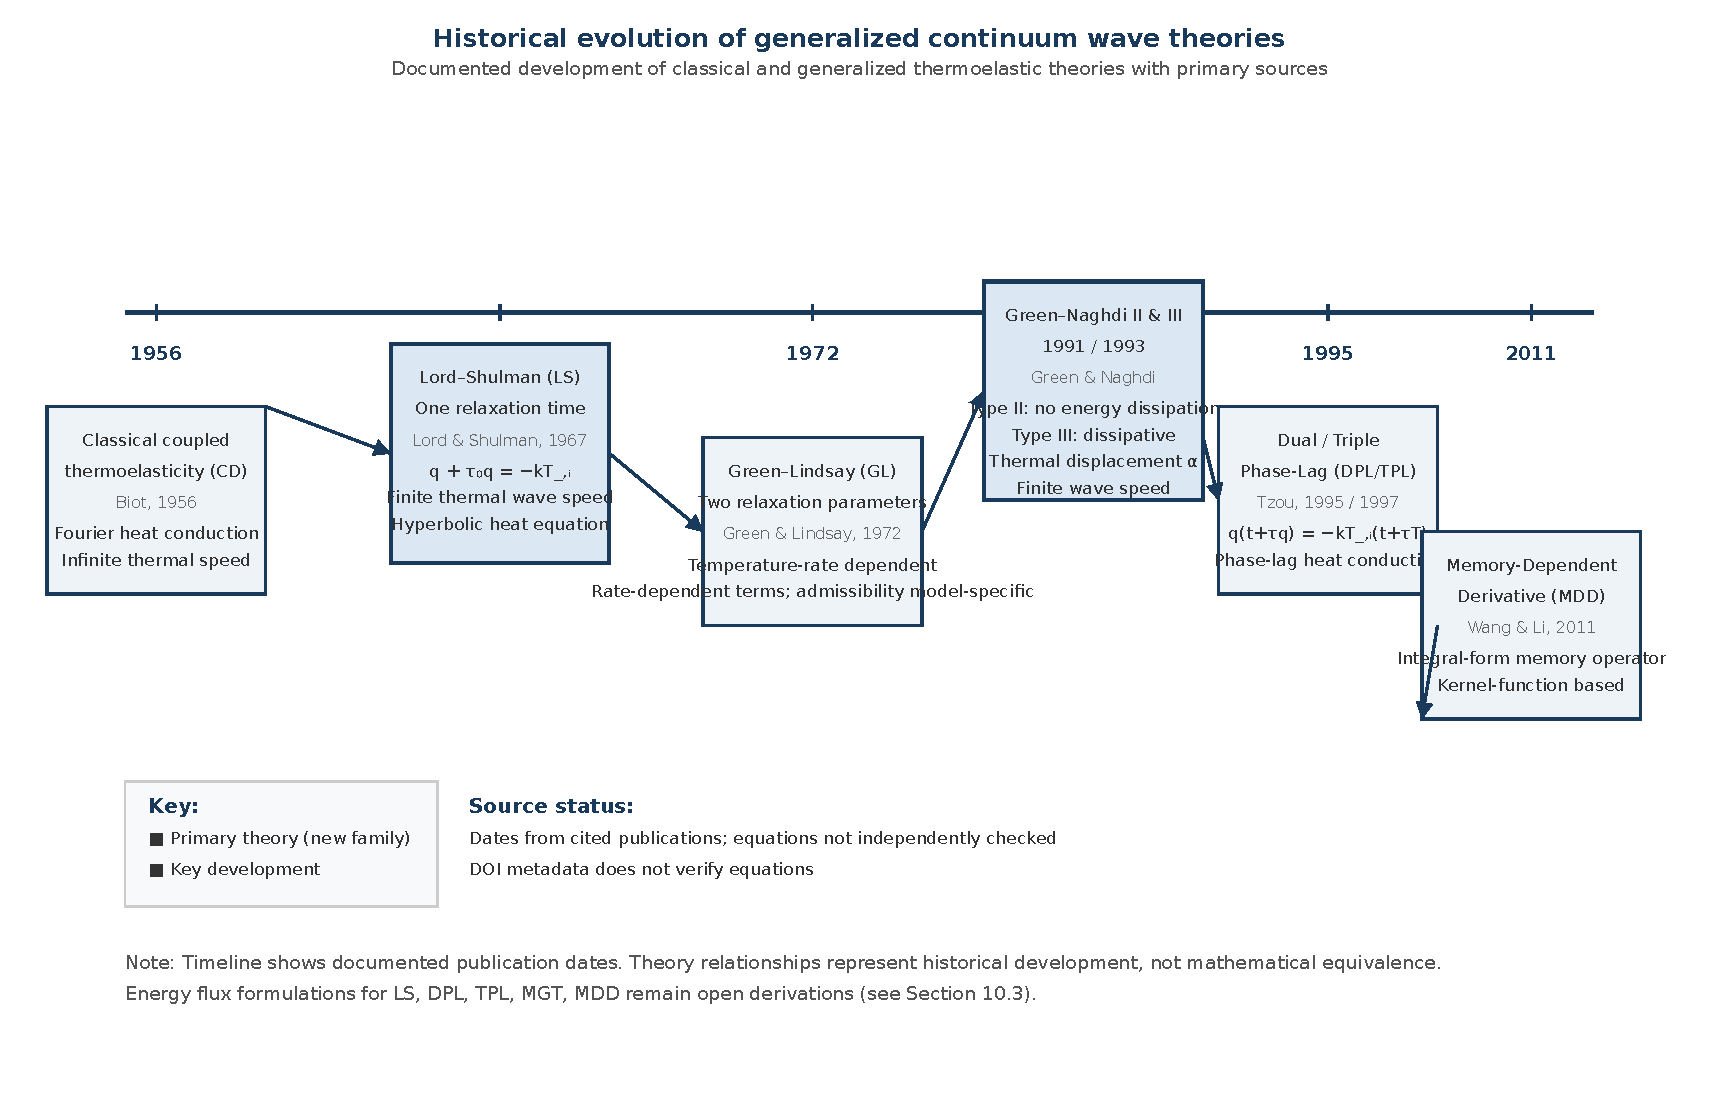
\includegraphics[width=0.9\textwidth]{fig01-theory-evolution.pdf}
\caption{Selected historical milestones in classical and generalized thermoelasticity. Publication dates and model descriptions are taken from the inherited bibliography; the figure does not assert that every generalized theory has finite propagation speed.}
\label{fig:theory_evolution}
\end{figure}

\begin{figure}[htbp]
\centering
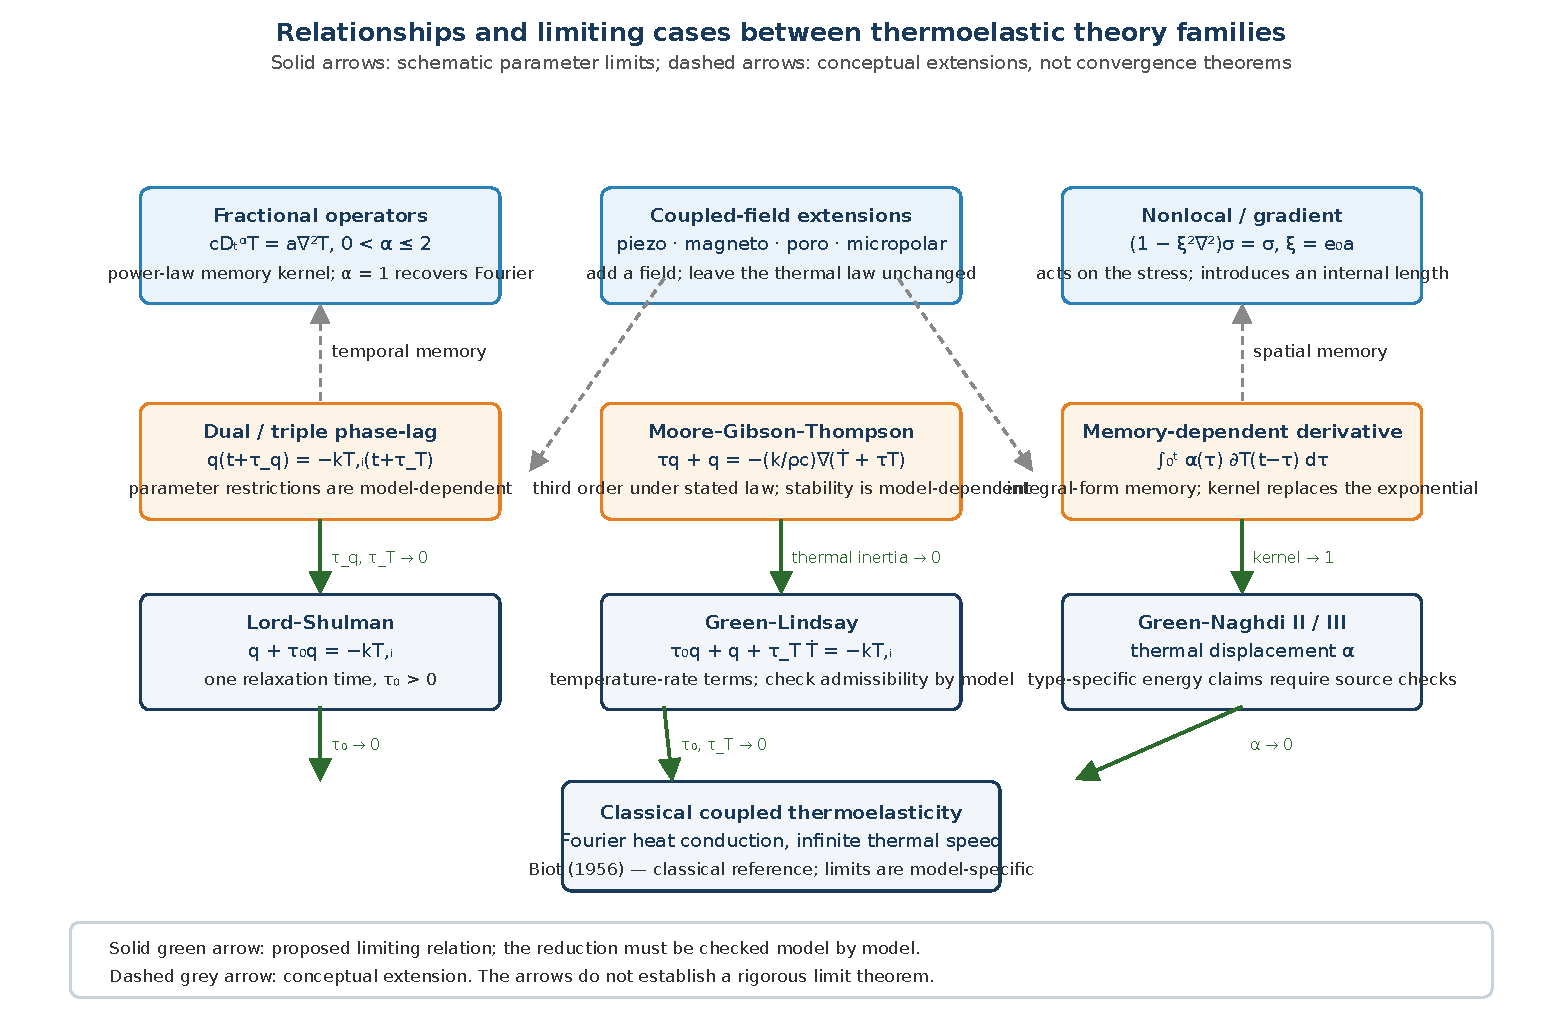
\includegraphics[width=0.9\textwidth]{fig02-theory-relationships.pdf}
\caption{Schematic relationships between thermoelastic model families. Parameter limits are model-specific and are not asserted to exist for every family; the arrows are conceptual rather than rigorous convergence results.}
\label{fig:theory_relationships}
\end{figure}

% LocalWords:


%======================================================================
% Section 2: Literature Strategy
%======================================================================
%======================================================================
% Section 2: Literature Landscape and Scholarly Context
%======================================================================
\section{Literature Landscape and Scholarly Context}
\label{sec:literature}

\subsection{The organising problem and the shape of the field}

The literature of generalized continuum wave mechanics addresses the infinite propagation speed associated with Fourier heat conduction. Joseph and Preziosi’s retrospective traces early finite-speed heat-flux formulations to Cattaneo and describes Vernotte’s later presentation of the relaxation law as a simple generalization \cite{Joseph1989}.

That pattern --- identification, modification, cost --- is the organising theme of this review, and it is why the literature is best read by theory family rather than by paper. Each family below answers the same question in a different way, and each pays for the answer in a different currency: a second temperature, a second wave, a loss of ellipticity, a loss of uniqueness, a loss of local well-posedness. Sections~\ref{sec:thermoelastic} through~\ref{sec:advanced} take the families in turn; this section establishes how they arose, where the field's centre of gravity has moved, and what the geographic distribution of the work reveals about the structure of the problem.

\subsection{Four phases in the development of the field}

Cattaneo and Vernotte proposed relaxation-type modifications of Fourier heat conduction; Lord and Shulman incorporated a relaxation time into coupled thermoelasticity. Green and Lindsay introduced a temperature-rate-dependent, single-temperature formulation with two relaxation parameters. These models have different constitutive structures and limiting assumptions.

\paragraph{Phase II --- second sound and thermal-displacement theories (1966--1993).} Phonon kinetic theory supplied a microscopic account of non-Fourier transport. Guyer and Krumhansl (1966) derived the phonon-Boltzmann structure and a nonlocal flux length scale; this is not treated as experimental evidence or a continuum thermoelastic law \cite{GuyerKrumhansl1966}. A separate companion paper, “Thermal Conductivity, Second Sound, and Phonon Hydrodynamic Phenomena in Nonmetallic Crystals,” begins at p. 778; it is distinct from the p. 766 article cited for the kinetic-theory equation above \cite{GuyerKrumhansl1966II}. The Green--Naghdi type-II primary formulation is the 1993 nondissipative theory, while the type-III equations are in the 1992 *Journal of Thermal Stresses* paper \cite{Green1993,GreenGN1992}. The type labels and dissipation statements below are limited to those specified systems; no universal Hamiltonian or energy claim is inferred. The synthesis of this phase is the review literature: Chandrasekharaiah's articles on hyperbolic thermoelasticity \cite{Chandrasekharaiah1986,Chandrasekharaiah1998}, Joseph and Preziosi's account of heat waves from kinetic theory to continuum mechanics \cite{Joseph1989,Joseph1990}, and the monographs by Nowacki \cite{Nowacki1975} and Achenbach \cite{Achenbach1973}.

\paragraph{Phase III --- the microscale turn (1995--2011).} Phase II assumed that the Fourier paradox was a matter of taking a limit too early. Phase III questioned the premise, and asked instead what a thermal wave should look like when the material has microstructure. Tzou's dual-phase-lag model \cite{Tzou1995} and Roy Choudhuri's triple-phase-lag formulation \cite{RoyChoudhuri2007} distinguish the flux and temperature-gradient lags and include a thermal-displacement-gradient contribution in the latter; the exact truncation and admissibility conditions remain model-specific. In parallel, Eringen's nonlocal elasticity \cite{Eringen1972,Eringen1974,Eringen1983} and the strain-gradient formulations \cite{Askes2006,Askes2011,Polizzotto2001} transferred the same logic to the mechanical side, and the size-dependent wave speeds measured and computed for nanostructures \cite{Maranganti2006,Maranganti2007} supplied the corresponding experimental evidence.

\paragraph{Phase IV --- memory, fractional operators and multiphysics (2011--present).} Recent models use memory kernels and coupled fields. Gorenflo and Mainardi provide mathematical background on fractional calculus \cite{Gorenflo1997}. Memory-dependent derivatives use time-history weights \cite{Wang2011}; fractional models replace integer-order derivatives with fractional orders in the governing equations \cite{Caputo1967,Povstenko2004,Povstenko2007,Povstenko2009,Povstenko2011,Povstenko2016}. Couplings to electrical, porous, micro-rotational, and carrier fields produce multiphysics formulations \cite{Iesan1986,Iesan2013,Cowin1983,Nunziato1979,Chandrasekharaiah1996,Marotti2013,Sharma2022,Abouelregal2023}.

\subsection{International structure of the field}

The development of generalized thermoelasticity involved several research communities. Foundational heat-conduction and thermoelasticity works, micropolar extensions, anisotropic models, fractional and memory-dependent formulations, and more recent multiphysics studies are represented in the cited literature \cite{Joseph1989,Biot1956,Lord1967,Green1972,Eringen1966a,Eringen1968b,Eringen1972,Dhaliwal1980,Sharma2022,Povstenko2004,Povstenko2007,Povstenko2009,Povstenko2011,Povstenko2016,Wang2011,Iesan1986,Iesan2013,Cowin1983,Nunziato1979,Chandrasekharaiah1996,Marotti2013,Abouelregal2023,Quintanilla2019,Barak2023,Barak2023IJP,Barak2023JTS,Barak2023MMMS,Gupta2023Energy,Gupta2023IJNMF,Kumar2023PhysScr,Gupta2026HeatMap}.

This distribution is not incidental. Each of the centres identified above entered the field through a different scientific interest --- heat conduction in metals, micropolar fluid mechanics, anomalous diffusion in geophysics, piezoelectricity in smart materials --- and each imported the constitutive modification appropriate to that interest. The result is a literature in which the same physical question, the admissibility of a propagating thermal mode, is attacked with structurally different devices: a relaxation time, a second temperature, a thermal displacement, a phase lag, a memory kernel, a fractional order. A review organised around papers would obscure this, because the same device reappears in every centre with different notation. A review organised around the devices --- which is what this review attempts --- shows that the field is not a sequence of independent advances but a single continuing negotiation between three requirements that are individually necessary and jointly expensive: finite propagation speed, thermodynamic admissibility, and well-posedness.

\subsection{The literature corpus}

The studies discussed here range from foundational analyses and surveys to applied work on coupled, nonlocal, fractional, and memory-dependent models. Comparisons are organized by constitutive structure and stated assumptions rather than by bibliographic metadata alone.

\subsection{Development axes and the gaps they expose}

The corpus can be classified along five axes --- physical domain, mathematical structure, modal content, coupling topology and validation regime --- and this classification is developed formally in Section~\ref{sec:taxonomy}. Its value at this stage is diagnostic: it shows where the field is dense and where it is thin. The dense regions are the single-field, one-dimensional, interface-focused problems of classical, relaxation-time and phase-lag thermoelasticity, for which a large body of modal and energy-ratio results exists. The thin regions are more revealing. There is very little work that closes the loop from constitutive novelty to experimental discrimination: the nonlocal and fractional families are theoretically mature, with well-established dispersion relations and modal structures, yet the number of studies that fit predictions to measured dispersion data remains small. The comparison of competing mechanisms for the same physical effect --- nonlocal versus gradient, exponential versus power-law memory, phase lag versus relaxation time --- is similarly under-represented, even though it is precisely in this comparison that the theory choices are testable. A third thin region is the treatment of interfaces in the presence of memory or nonlocality, where the constitutive history and the geometric matching condition must be reconciled, and where the energy partition is not determined by the local constitutive law.

These gaps are not defects of the individual contributions; they follow from the structure of the field, in which each advance has been made by extending a constitutive law and then solving the resulting modal problem, and the natural next step --- putting two such extensions in competition against an experiment --- has not yet become the standard mode of work. Section~\ref{sec:future} takes this diagnosis as the basis for its research directions.

\subsection{Existing reviews and the contribution of this article}

Reviews already exist for several individual theory families: nonlocal elasticity and its application to nanostructures \cite{Askes2006,Askes2011,Maranganti2007}, fractional thermoelasticity \cite{Chandrasekharaiah1998,Povstenko2016}, hyperbolic thermoelasticity and second sound \cite{Chandrasekharaiah1996,Joseph1989}, and generalized thermoelasticity with modified models \cite{Shakeriaski2021}. Their common structure is the one this review sets aside: an enumeration of theory families, each with its governing equations, its application domains and a list of its principal results, with the families treated in isolation and the transitions between them left implicit.

The present review differs in three respects. It is organised by the problems --- finite propagation speed, thermodynamic admissibility, well-posedness, scale dependence, interface partition of energy --- rather than by the theories, so that a reader interested in one problem can follow it across all the theories that address it. It states the cost of each modification alongside the benefit, which the standard format does not do, and which the literature itself rarely does: the second temperature, the loss of ellipticity, the loss of uniqueness of the initial-value problem, and the non-locality of the energy flux are each the price of something that was bought. It separates a mechanism's plausibility from the empirical support for it, treating the evidence base as an explicit axis of classification rather than a matter of emphasis.

\begin{figure}[htbp]
\centering
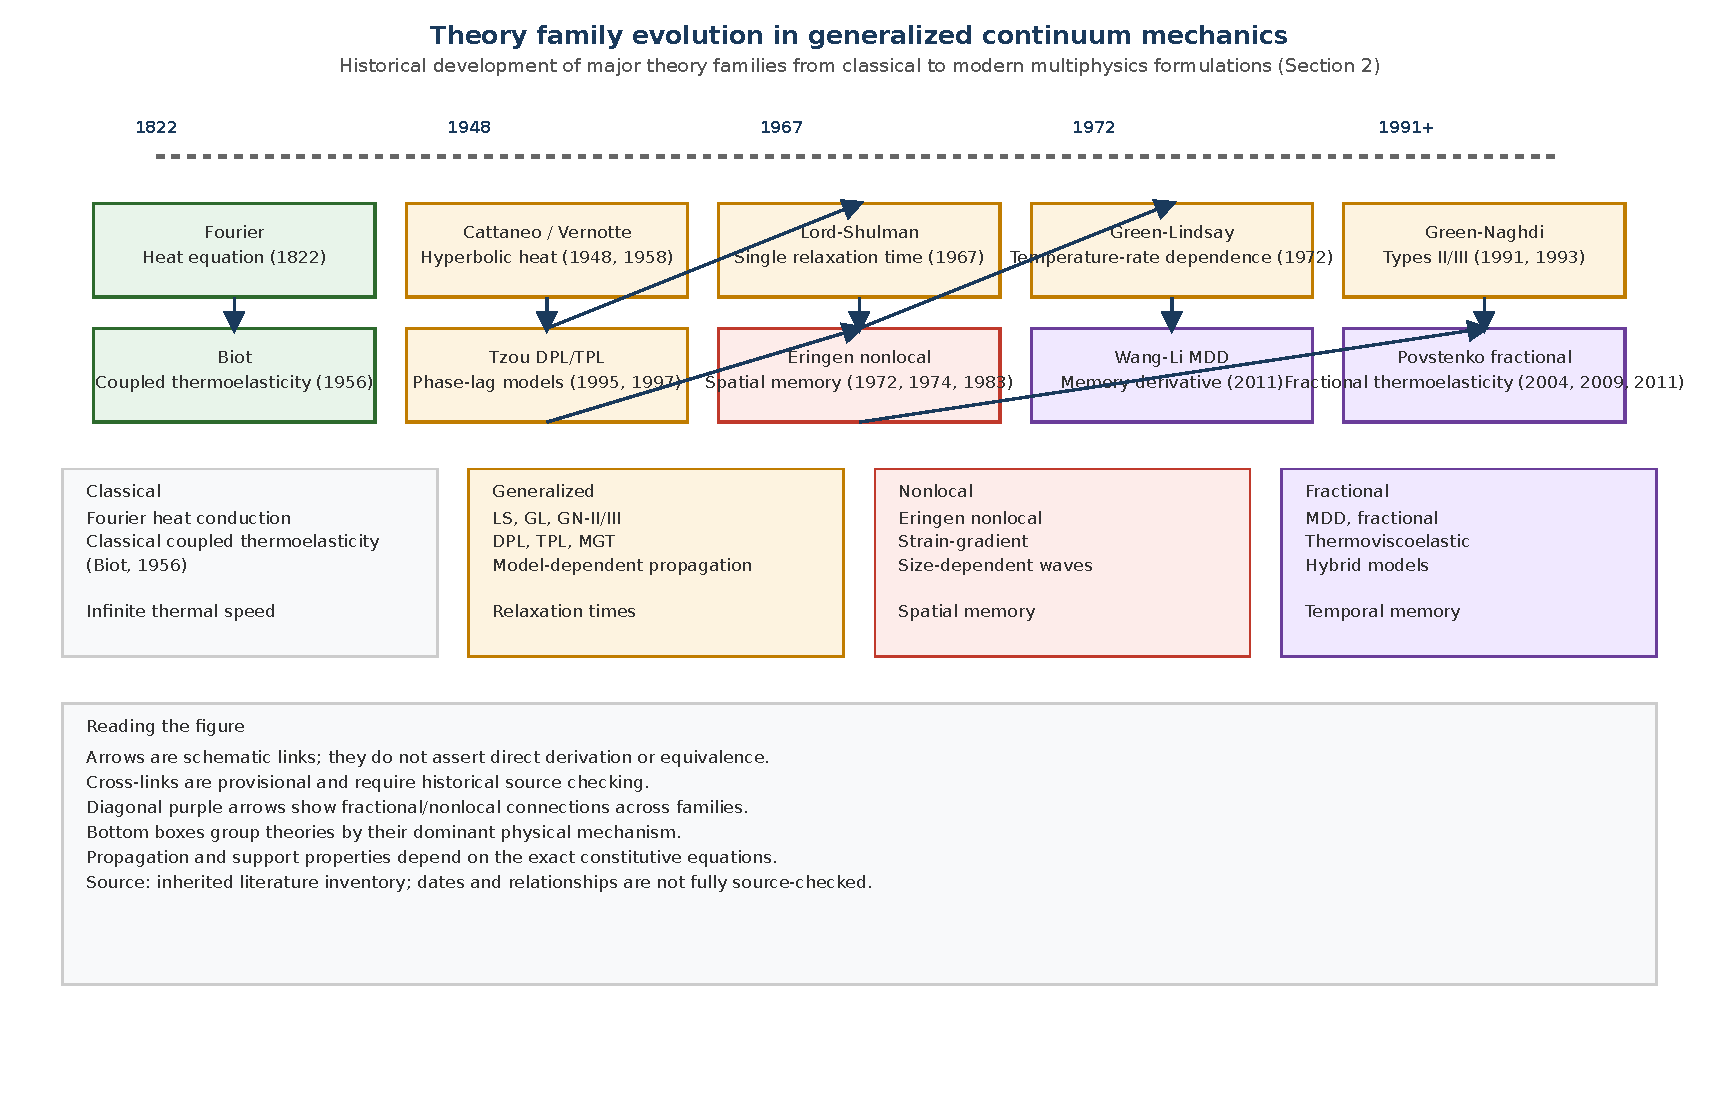
\includegraphics[width=0.95\textwidth]{fig03-literature-landscape.pdf}
\caption{Selected theory families and relationships in generalized continuum mechanics. This schematic is a conceptual taxonomy of the model families discussed in the text.}
\label{fig:literature_landscape}
\end{figure}

\subsection{Citation and assumptions}

A useful comparison states the validity domain and conventions of each equation and distinguishes a derivation from an attributed result. The assumptions used in each cited formulation are therefore identified alongside the relevant discussion.

Where material errors are conclusively established in the literature, they are recorded transparently and without personal characterisation. Where uncertainty exists, it is acknowledged as an open question. No error allegations are made against any publication, and model-specific differences are never presented as mathematical contradictions without sufficient evidence.

% LocalWords:


%======================================================================
% Section 3: Foundations of Continuum Wave Mechanics
%======================================================================
%======================================================================
% Section 3: Foundations of Continuum Wave Mechanics
%======================================================================
\section{Foundations of Continuum Wave Mechanics}
\label{sec:foundations}

This section develops the first-principles foundation (Layer I of the layered mathematical exposition) for all subsequent theory families. We begin with kinematics, proceed through the conservation laws of continuum mechanics, establish the thermodynamic restrictions on constitutive relations, derive classical elasticity and wave propagation, and conclude with the classical energy flux \cite{Biot1956} and interface conditions. Every equation in this section is derived from first principles or drawn from established standard results with documented assumptions.

\subsection{Kinematics: displacement, strain, rotation}
\label{sec:3.1}

Let $\bm{u}(\bm{x},t)$ denote the displacement field of a continuum body occupying a region $\Omega \subset \mathbb{R}^3$ with boundary $\partial\Omega$. The displacement gradient tensor decomposes additively into symmetric and antisymmetric parts:

\begin{equation}
u_{i,j} = \varepsilon_{ij} + \omega_{ij},
\label{eq:3.1}
\end{equation}

where the infinitesimal strain tensor and rotation tensor are defined by

\begin{equation}
\varepsilon_{ij} = \frac{1}{2}(u_{i,j} + u_{j,i}),
\qquad
\omega_{ij} = \frac{1}{2}(u_{i,j} - u_{j,i}).
\label{eq:3.2}
\end{equation}

The strain tensor $\varepsilon_{ij}$ measures the symmetric part of the displacement gradient (deformation), while the rotation tensor $\omega_{ij}$ measures the antisymmetric part (rigid-body rotation). The velocity field is the material time derivative of displacement:

\begin{equation}
v_i = \dot{u}_i = \frac{\partial u_i}{\partial t}.
\label{eq:3.3}
\end{equation}

\subsubsection{Physical interpretation}
The strain components $\varepsilon_{ii}$ represent normal strains (relative changes in length along coordinate directions), while $\varepsilon_{ij}$ ($i \neq j$) represent shear strains (changes in angle between originally orthogonal material lines). The infinitesimal strain assumption requires $\|\varepsilon_{ij}\| \ll 1$, which is valid for small deformations typical of linearized wave propagation problems.

\begin{figure}[htbp]
\centering
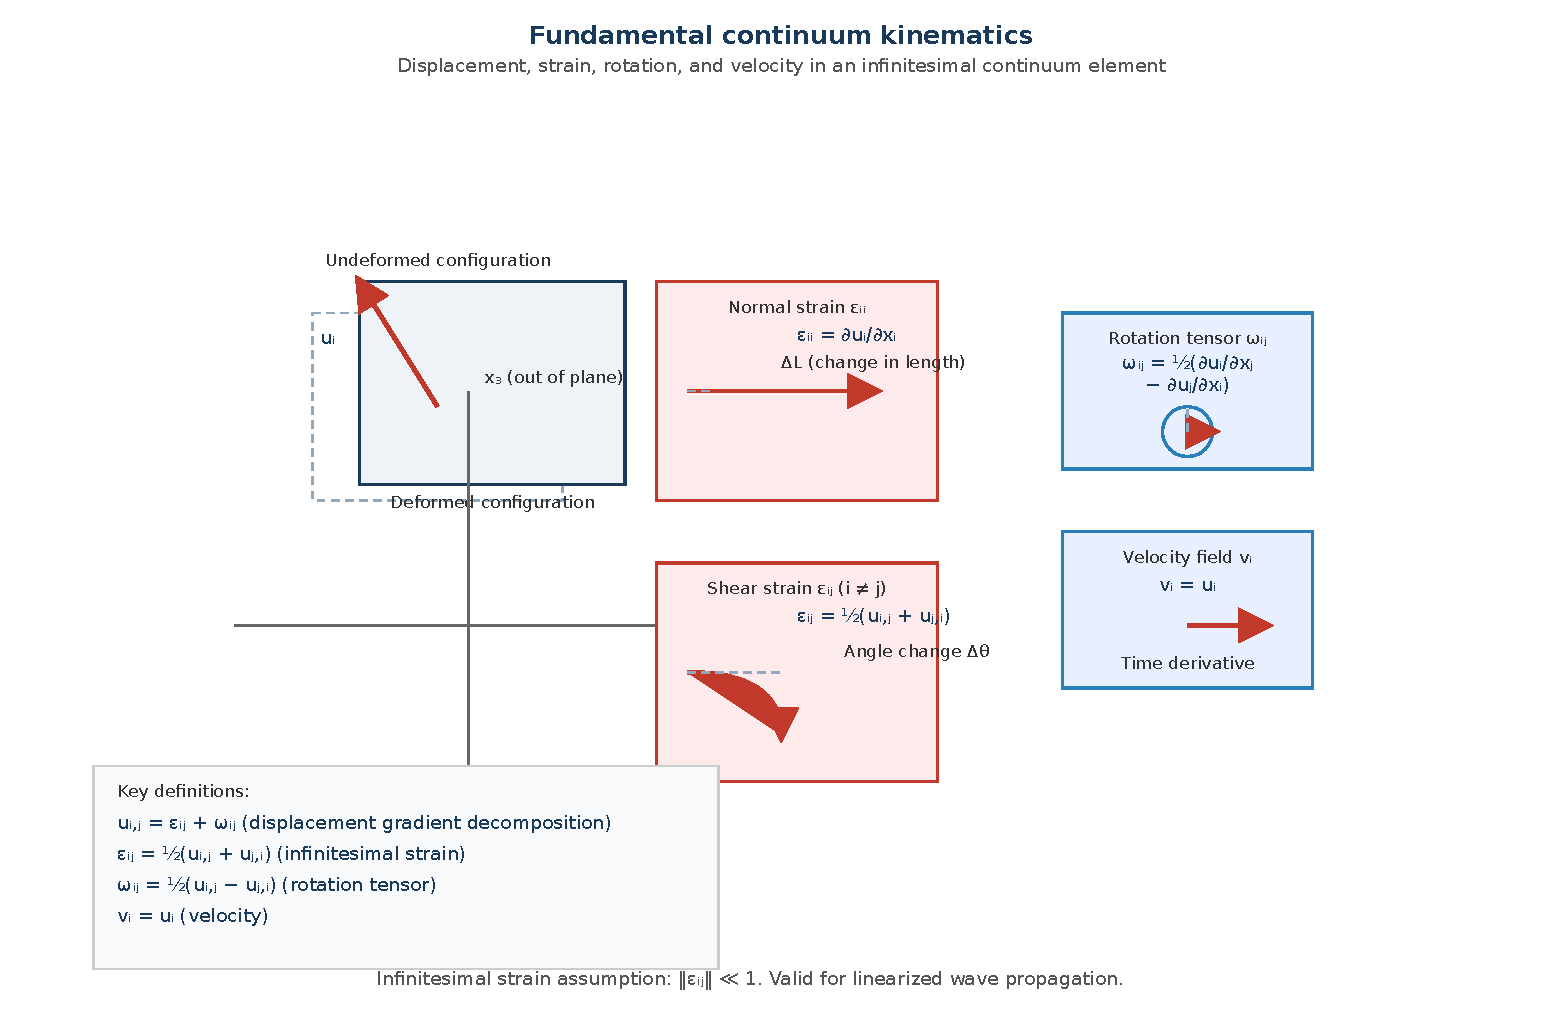
\includegraphics[width=0.9\textwidth]{fig04-continuum-kinematics.pdf}
\caption{Kinematics of a continuum element. The displacement field $\bm{u}(\bm{x},t)$ defines the deformation gradient, which in the infinitesimal regime splits additively into a symmetric part (strain, the extensional part of the deformation) and an antisymmetric part (rotation, the rigid part). The rigid part does no work and is removed from the balance laws by the objectivity requirement, so that only the strain enters the stress; this is the first of the two places where irreversibility enters the formulation, the second being the second law of Section~\ref{sec:3.4}.}
\label{fig:kinematics}
\end{figure}

\subsection{Conservation laws: linear momentum and angular momentum}
\label{sec:3.2}

\subsubsection{Linear momentum balance}

Consider a material subvolume $V \subset \Omega$ with surface $S = \partial V$ and outward unit normal $\bm{n}$. The linear momentum balance states that the time rate of change of linear momentum equals the sum of surface tractions and body forces:

\begin{equation}
\frac{\diff}{\diff t} \int_V \rho v_i \, \diff V
=
\int_S \sigma_{ji} n_j \, \diff S
+
\int_V \rho f_i \, \diff V,
\label{eq:3.4}
\end{equation}

where $\rho$ is the mass density, $\sigma_{ji}$ is the Cauchy stress tensor, and $f_i$ is the body force per unit mass. Applying the divergence theorem to the surface integral and localizing (since $V$ is arbitrary) yields the pointwise form:

\begin{equation}
\rho \dot{v}_i = \sigma_{ji,j} + \rho f_i.
\label{eq:3.5}
\end{equation}

Since $v_i = \dot{u}_i$, this can also be written in terms of displacement:

\begin{equation}
\rho \ddot{u}_i = \sigma_{ji,j} + \rho f_i.
\label{eq:3.6}
\end{equation}

Equation \eqref{eq:3.5} is the fundamental equation of motion for continuum mechanics. It is sometimes called Cauchy's first law or the equation of linear momentum.

\subsubsection{Angular momentum balance}

The angular momentum balance for an arbitrary subvolume $V$ states:

\begin{equation}
\frac{\diff}{\diff t} \int_V \rho (\bm{x} \times \bm{v})_k \, \diff V
=
\int_S \epsilon_{kij} x_i \sigma_{jm} n_m \, \diff S
+
\int_V \rho \epsilon_{kij} x_i f_j \, \diff V,
\label{eq:3.7}
\end{equation}

where $\epsilon_{kij}$ is the Levi-Civita permutation symbol. Applying the divergence theorem, using the linear momentum balance \eqref{eq:3.5}, and localizing gives:

\begin{equation}
\sigma_{ij} = \sigma_{ji}.
\label{eq:3.8}
\end{equation}

Equation \eqref{eq:3.8} states that the Cauchy stress tensor is symmetric in the absence of couple stresses or body couples. This symmetry is essential for the energy flux derivations in Sections 3.8 and 10.2.

\subsubsection{Physical interpretation}
Equations \eqref{eq:3.5} and \eqref{eq:3.8} are local statements of Newton's second law applied to continuum matter. The symmetry of stress (\eqref{eq:3.8}) means that traction on a surface is determined solely by the normal to that surface, without additional rotational degrees of freedom in classical (non-polar) continua.

\subsection{Mechanical power and internal energy: first law of thermodynamics}
\label{sec:3.3}

\subsubsection{Mechanical power balance}

Multiply the linear momentum equation \eqref{eq:3.5} by $v_i$ and integrate over $V$:

\begin{equation}
\int_V \rho \dot{v}_i v_i \, \diff V
=
\int_V \sigma_{ji,j} v_i \, \diff V
+
\int_V \rho f_i v_i \, \diff V.
\label{eq:3.9}
\end{equation}

The left-hand side is the rate of change of kinetic energy:

\begin{equation}
\int_V \rho \dot{v}_i v_i \, \diff V
=
\frac{\diff}{\diff t} \int_V \frac{1}{2}\rho v_i v_i \, \diff V.
\label{eq:3.10}
\end{equation}

For the stress term, use the identity $\sigma_{ji,j}v_i = (\sigma_{ji}v_i)_{,j} - \sigma_{ji}v_{i,j}$. Since $v_{i,j} = \dot{u}_{i,j} = \dot{\varepsilon}_{ji}$ (using symmetry of $\sigma_{ji}$ and $\varepsilon_{ij}$), we obtain:

\begin{equation}
\int_V \sigma_{ji,j} v_i \, \diff V
=
\int_S \sigma_{ji} v_i n_j \, \diff S
-
\int_V \sigma_{ji} \dot{\varepsilon}_{ij} \, \diff V.
\label{eq:3.11}
\end{equation}

Combining \eqref{eq:3.9} through \eqref{eq:3.11} gives the mechanical power balance:

\begin{equation}
\rho \frac{\diff}{\diff t}\left(\frac{1}{2}v_i v_i\right)
=
\sigma_{ji,j}v_i + \rho f_i v_i
=
-\sigma_{ij}\dot{\varepsilon}_{ij} + (\sigma_{ij}v_j)_{,i} + \rho f_i v_i.
\label{eq:3.12}
\end{equation}

The term $\sigma_{ij}v_j n_i$ on the surface represents mechanical power entering through the boundary per unit area; its density $(\sigma_{ij}v_j)_{,i}$ is the mechanical power flux divergence.

\subsubsection{Internal energy balance}

The first law of thermodynamics for a continuum states that the rate of change of internal energy equals the mechanical power input minus the heat flux out of the body plus heat supply:

\begin{equation}
\rho \dot{e} = \sigma_{ij}\dot{\varepsilon}_{ij} - q_{i,i} + \rho r,
\label{eq:3.13}
\end{equation}

where $e$ is the specific internal energy (per unit mass), $q_i$ is the heat flux vector, and $r$ is the heat supply per unit mass. In the absence of external heat supply ($r = 0$):

\begin{equation}
\rho \dot{e} = \sigma_{ij}\dot{\varepsilon}_{ij} - q_{i,i}.
\label{eq:3.14}
\end{equation}

\subsubsection{Physical interpretation}
Equation \eqref{eq:3.13} expresses energy conservation: the internal energy of a material element changes due to (i) mechanical work done by stresses ($\sigma_{ij}\dot{\varepsilon}_{ij}$), (ii) heat conduction out of the element ($-q_{i,i}$), and (iii) external heat supply ($\rho r$). The term $\sigma_{ij}\dot{\varepsilon}_{ij}$ is the stress power density — the rate of mechanical work converted into internal energy or stored as elastic energy.

\subsection{Entropy and dissipation inequality: Clausius--Duhem inequality}
\label{sec:3.4}

The second law of thermodynamics, in the Clausius--Duhem form, states that the entropy production within a continuum is non-negative:

\begin{equation}
\rho \dot{s} \geq -\left(\frac{q_i}{\Theta}\right)_{,i} + \frac{\rho r}{\Theta},
\label{eq:3.15}
\end{equation}

where $s$ is specific entropy and $\Theta$ is absolute temperature. In the linear constitutive equations below, $T=\Theta-T_0$ denotes the temperature increment. Using the internal-energy balance \eqref{eq:3.13} and defining the Helmholtz free energy by $\psi=e-\Theta s$, we obtain after standard manipulation:

\begin{equation}
\sigma_{ij}\dot{\varepsilon}_{ij} - \rho\left(\dot{\psi} + s\dot{\Theta}\right) - \frac{q_i \Theta_{,i}}{\Theta} \geq 0.
\label{eq:3.16}
\end{equation}

Equation \eqref{eq:3.16} is the Clausius--Duhem dissipation inequality. The left-hand side represents the local entropy production rate (multiplied by temperature) and must be non-negative for all admissible thermodynamic processes.

\subsubsection{Physical interpretation}
The dissipation inequality restricts admissible constitutive relations. Any constitutive model must be constructed so that \eqref{eq:3.16} holds for all processes. This principle is used in Section 3.5 to derive Coleman--Noll restrictions and in Section 10.7 to assess thermodynamic admissibility of generalized theories.

\subsection{Constitutive principles: free energy and linear relations}
\label{sec:3.5}

\subsubsection{Coleman--Noll procedure}

Assuming the free energy depends on strain and temperature, $\psi = \psi(\varepsilon_{ij}, T)$, we have:

\begin{equation}
\dot{\psi} = \frac{\partial\psi}{\partial\varepsilon_{ij}}\dot{\varepsilon}_{ij}
+ \frac{\partial\psi}{\partial T}\dot{T}.
\label{eq:3.17}
\end{equation}

Substituting into the dissipation inequality \eqref{eq:3.16} and requiring it to hold for arbitrary $\dot{\varepsilon}_{ij}$ and $\dot{T}$ yields the Coleman--Noll restrictions:

\begin{equation}
\sigma_{ij} = \rho \frac{\partial\psi}{\partial\varepsilon_{ij}},
\qquad
s = -\frac{\partial\psi}{\partial T}.
\label{eq:3.18}
\end{equation}

With these restrictions, the dissipation inequality reduces to the thermal conduction restriction:

\begin{equation}
-\frac{q_i T_{,i}}{T} \geq 0.
\label{eq:3.19}
\end{equation}

For isotropic linear conduction with Fourier's law $q_i = -k T_{,i}$ ($k > 0$), we have $-q_i T_{,i}/T = k(T_{,i})^2/T \geq 0$, which is satisfied.

\subsubsection{Linear isotropic constitutive relations}

For a linear isotropic thermoelastic material, with temperature increment $T=\Theta-T_0$ and thermal-stress coefficient $\beta$ in Pa K$^{-1}$, take the specific Helmholtz free energy:

\begin{equation}
\psi = \frac{1}{2\rho}(\lambda \varepsilon_{kk}\varepsilon_{ll} + 2\mu \varepsilon_{ij}\varepsilon_{ij})
- \frac{\beta}{\rho}\varepsilon_{kk} T - s_0 T - \frac{c_v}{2 T_0}T^2 + \text{const.},
\label{eq:3.20}
\end{equation}

where $\lambda$ and $\mu$ are Lamé elastic constants, $\beta$ is the thermal stress coefficient, and $c_v$ is the specific heat at constant strain. Applying \eqref{eq:3.18} gives:

\begin{equation}
\sigma_{ij} = \lambda \varepsilon_{kk}\delta_{ij} + 2\mu\varepsilon_{ij} - \beta T\delta_{ij},
\label{eq:3.21}
\end{equation}

\begin{equation}
s = s_0 + \frac{\beta}{\rho}\varepsilon_{kk} + \frac{c_v}{T_0}T.
\label{eq:3.22}
\end{equation}

Equation \eqref{eq:3.21} is the linear isotropic thermoelastic constitutive relation: the first two terms are the classical elastic stress (Hooke's law), and the last term is the thermal stress contribution.

\subsubsection{Physical interpretation}
The constitutive relations \eqref{eq:3.21}--\eqref{eq:3.22} couple mechanical and thermal fields: temperature changes induce thermal stresses ($-\beta T\delta_{ij}$), and deformation changes entropy ($\frac{\beta}{\rho}\varepsilon_{kk}$). This coupling is the physical origin of thermoelastic wave propagation.

\subsection{Classical elasticity: Navier equations and wave speeds}
\label{sec:3.6}

Substituting the constitutive relation \eqref{eq:3.21} into the equation of motion \eqref{eq:3.6} with no body forces ($f_i = 0$) and isothermal conditions ($T = T_0$ constant), we obtain the Navier equations of classical elasticity:

\begin{equation}
\rho\ddot{u}_i = (\lambda + \mu)u_{j,ji} + \mu u_{i,jj}.
\label{eq:3.23}
\end{equation}

\subsubsection{Plane wave solutions}

For harmonic plane waves of the form $u_i = \hat{u}_i e^{i(\bm{k}\cdot\bm{x} - \omega t)}$, substitution into \eqref{eq:3.23} gives the Christoffel equation. For longitudinal (P) waves propagating in direction $\bm{n}$ with polarization parallel to $\bm{n}$:

\begin{equation}
c_p = \sqrt{\frac{\lambda + 2\mu}{\rho}},
\label{eq:3.24}
\end{equation}

and for transverse (S or SV) waves with polarization perpendicular to $\bm{n}$:

\begin{equation}
c_s = \sqrt{\frac{\mu}{\rho}}.
\label{eq:3.25}
\end{equation}

These are the classical elastic wave speeds. The P-wave speed exceeds the S-wave speed since $\lambda + 2\mu > \mu$ for stable materials ($\lambda + 2\mu/3 > 0$, $\mu > 0$).

\subsubsection{Physical interpretation}
Equation \eqref{eq:3.23} describes how elastic disturbances propagate through a homogeneous isotropic solid. The P-wave involves volume change (compressional), while the S-wave involves shear (distortional) deformation. Both propagate without dispersion in classical elasticity — all frequencies travel at the same speed.

\begin{figure}[htbp]
\centering
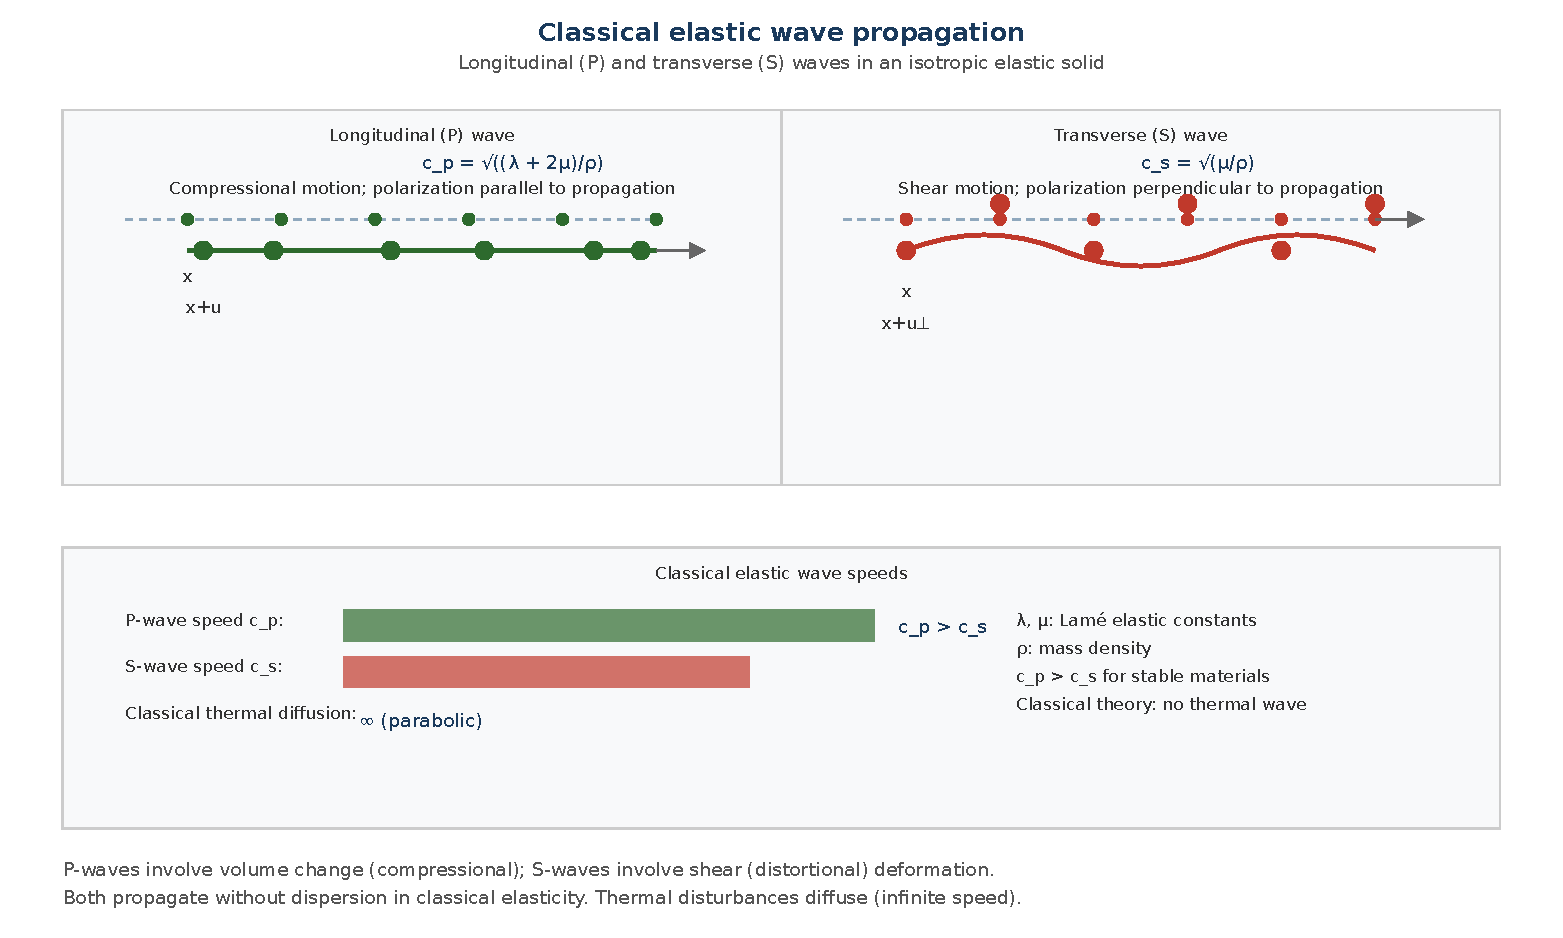
\includegraphics[width=0.95\textwidth]{fig06-classical-waves.pdf}
\caption{Classical elastic wave propagation in an isotropic solid. A longitudinal (P) wave, whose polarization is parallel to the propagation direction, travels at $c_p = \sqrt{(\lambda + 2\mu)/\rho}$; a transverse (S) wave, whose polarization is perpendicular to it, travels at $c_s = \sqrt{\mu/\rho}$. Because the elastic moduli are independent of frequency, both speeds are dispersion-free: this constancy is the reference against which the dispersive branches of Sections~4--7 are measured, and it is the property that a generalized theory must forfeit when it introduces a length scale or a memory kernel.}
\label{fig:classical_waves}
\end{figure}

\subsection{Plane wave assumptions and harmonic wave form}
\label{sec:3.7}

For time-harmonic problems, all field variables take the form:

\begin{equation}
u_i(\bm{x},t) = \hat{u}_i(\bm{x}) e^{-i\omega t},
\qquad
\sigma_{ij}(\bm{x},t) = \hat{\sigma}_{ij}(\bm{x}) e^{-i\omega t},
\qquad
q_i(\bm{x},t) = \hat{q}_i(\bm{x}) e^{-i\omega t},
\label{eq:3.26}
\end{equation}

where $\hat{u}_i$, $\hat{\sigma}_{ij}$, $\hat{q}_i$ are complex amplitudes and $\omega$ is the angular frequency. The time convention $e^{-i\omega_t}$ implies that positive imaginary parts of complex wave numbers correspond to attenuation (decay in space) and negative imaginary parts of complex frequencies correspond to temporal decay.

\subsubsection{Time-average identity}

For two harmonic quantities $a(t) = \Re[\hat{a} e^{-i\omega t}]$ and $b(t) = \Re[\hat{b} e^{-i\omega t}]$, the time average over one period is:

\begin{equation}
\avg{ab}_t = \frac{1}{2}\Re[\hat{a}\hat{b}^*],
\label{eq:3.27}
\end{equation}

where $^*$ denotes complex conjugation. This identity is used throughout Sections 9 and 10 to compute average energy fluxes and energy ratios from complex wave amplitudes.

\subsection{Energy flux in classical elasticity}
\label{sec:3.8}

Adding the mechanical power balance \eqref{eq:3.12} and the internal-energy balance \eqref{eq:3.14} (with $r=0$), and defining total energy per unit volume as $\mathcal{E}=\frac12\rho v_i v_i+\rho e$, gives an outward-positive flux $J_j=q_j-\sigma_{ji}v_i$:

\begin{equation}
\frac{\partial\mathcal{E}}{\partial t}
+
\frac{\partial}{\partial x_j}\left(q_j - \sigma_{ji}v_i\right)
=
\rho f_i v_i.
\label{eq:3.28}
\end{equation}

With no body forces ($f_i = 0$), this becomes the local energy conservation law:

\begin{equation}
\frac{\partial\mathcal{E}}{\partial t} + \frac{\partial J_i}{\partial x_i} = 0,
\qquad
J_i = q_i - \sigma_{ij}v_j.
\label{eq:3.29}
\end{equation}

Equation \eqref{eq:3.29} states that the total energy density changes only due to the divergence of the energy flux $J_i$. The energy flux has two contributions:

\begin{itemize}
\item $-\sigma_{ij}v_j$: mechanical contribution to the outward-positive flux, and
\item $q_i$: thermal energy flux (heat conduction across a surface per unit area).
\end{itemize}

Integrating \eqref{eq:3.29} over a volume $V$ and applying the divergence theorem:

\begin{equation}
\frac{\diff}{\diff t}\int_V \mathcal{E} \, \diff V
+
\int_S J_i n_i \, \diff S = 0.
\label{eq:3.30}
\end{equation}

For an isolated system ($J_i n_i = 0$ on $S$), the total energy is conserved: $\frac{\diff}{\diff t}\int_V \mathcal{E} \, \diff V = 0$.

\subsubsection{Physical interpretation}
Equation \eqref{eq:3.29} is the classical energy flux \cite{Biot1956} for elastic and thermoelastic media. With the outward-positive convention, the mechanical contribution is $-\sigma_{ij}v_j$ and the thermal contribution is $q_i$. Reversing the normal or defining inward-positive flux reverses the signs consistently. This local balance is derived for the classical thermoelastic model only. Whether an additional stored-energy or boundary-power term is required in a generalized theory depends on its constitutive equations and must be derived model by model.

\begin{figure}[htbp]
\centering
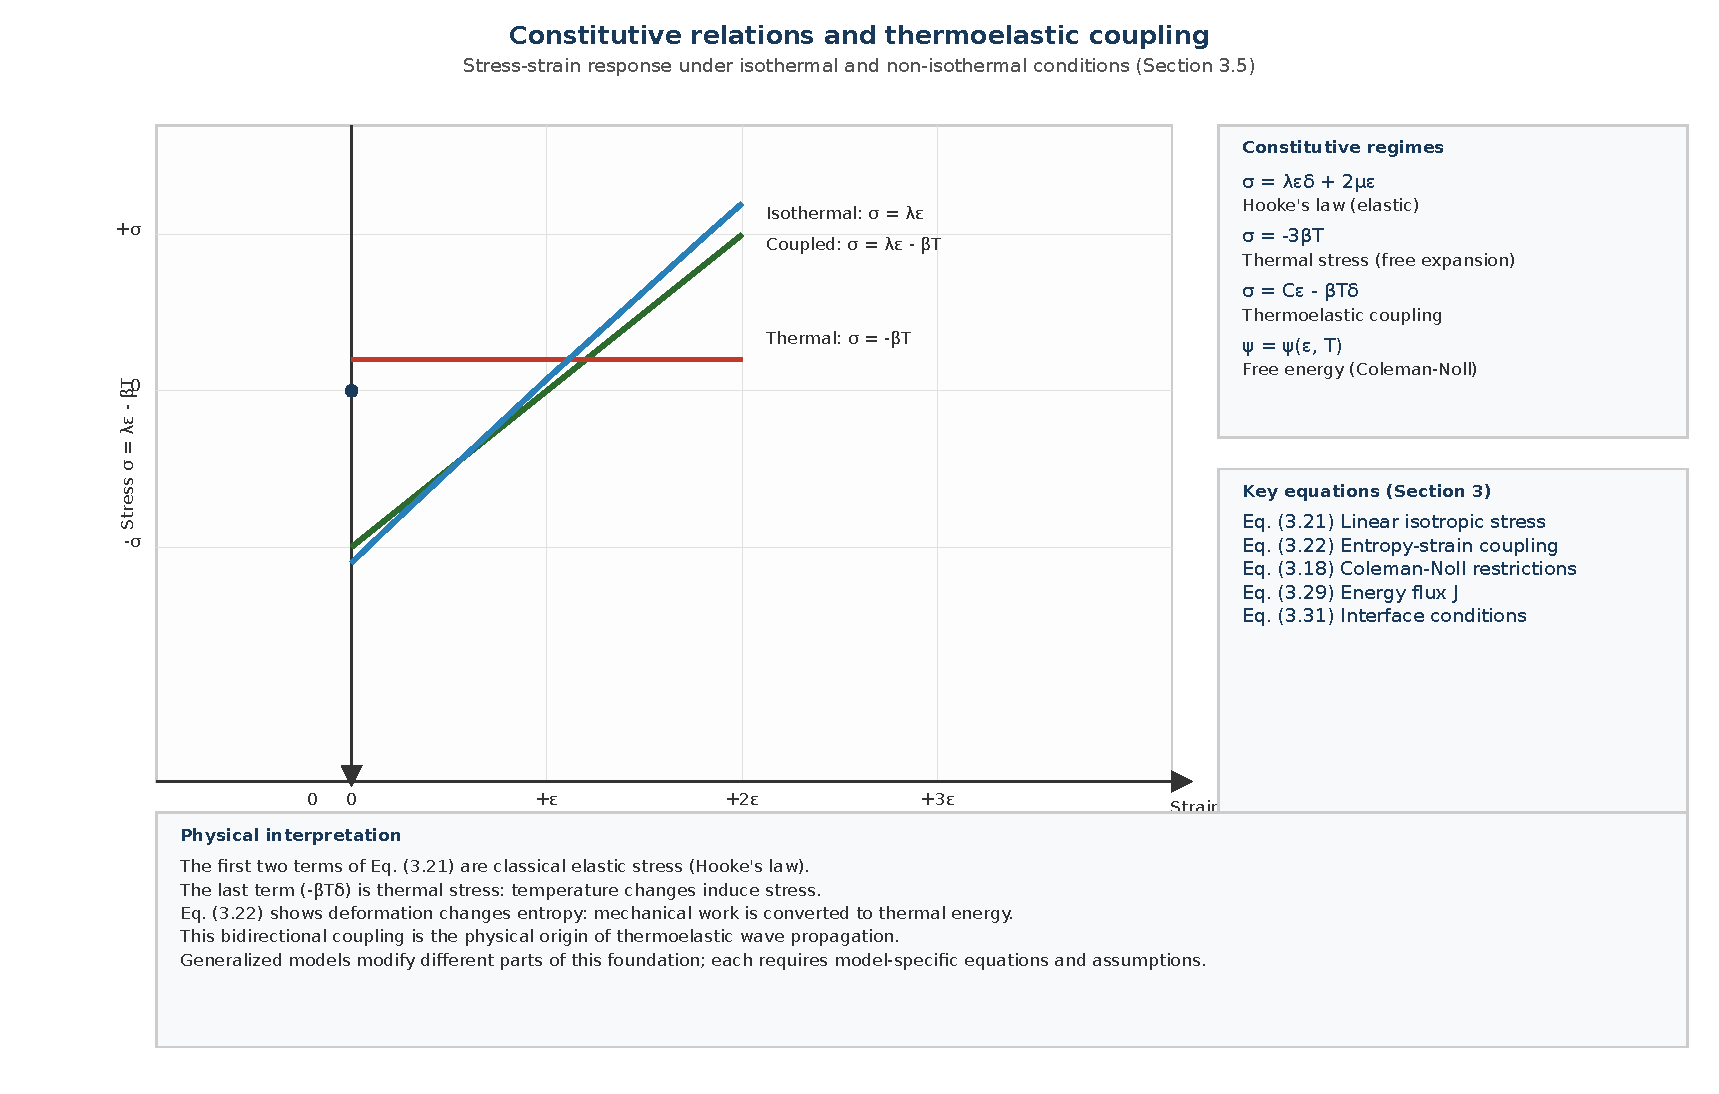
\includegraphics[width=0.95\textwidth]{fig05-constitutive-relations.pdf}
\caption{Constitutive relations and thermoelastic coupling: stress-strain response under isothermal and non-isothermal conditions (Section 3.5).}
\label{fig:constitutive}
\end{figure}

\subsection{Interface conditions: perfect and imperfect bonding}
\label{sec:3.9}

Consider an interface $\Sigma$ between two media (denoted $1$ and $2$) with common unit normal $\bm{n}$. For perfectly bonded interfaces:

\subsubsection{Perfect bonding}

\begin{equation}
u_i^{(1)} = u_i^{(2)},
\qquad
\sigma_{ji}^{(1)}n_j = \sigma_{ji}^{(2)}n_j,
\qquad
T^{(1)} = T^{(2)},
\qquad
q_i^{(1)}n_i = q_i^{(2)}n_i,
\label{eq:3.31}
\end{equation}

on $\Sigma$. The first condition enforces displacement continuity (no slip or separation), the second enforces traction equilibrium (Newton's third law at the interface), and the last two enforce thermal contact (temperature continuity and heat flux continuity).

\subsubsection{Imperfect bonding: spring-type conditions}

For imperfectly bonded interfaces, displacement and traction are related by interfacial stiffness parameters:

\begin{equation}
[u_i] = (C^u)^{-1}_{ij} t_j,
\qquad
\sigma_{ki}^{(1)}n_k = \sigma_{ki}^{(2)}n_k = t_i,
\label{eq:3.32}
\end{equation}

where $[u_i]=u_i^{(2)}-u_i^{(1)}$, $t_i$ is the common traction on the shared normal, and $C^u_{ij}$ is a positive-definite interfacial stiffness tensor (units Pa/m). The compliance form is used so that, when all stiffness eigenvalues tend to infinity, the displacement jump vanishes; when they tend to zero through positive values, the traction vanishes for a finite jump. More general imperfect-interface laws require their own constitutive and dissipation assumptions.

\subsubsection{Electrical interface conditions (piezoelectric media)}

For piezoelectric media, additional interface conditions involve the electric potential $\phi$ and electric displacement $D_i$:

\begin{equation}
\phi^{(1)} = \phi^{(2)}
\qquad \text{(perfect electrical contact)},
\label{eq:3.33}
\end{equation}

\begin{equation}
D_i^{(1)}n_i = D_i^{(2)}n_i
\qquad \text{(electric displacement continuity)},
\label{eq:3.34}
\end{equation}

or for an insulated interface:

\begin{equation}
D_i n_i = 0.
\label{eq:3.35}
\end{equation}

\subsubsection{Physical interpretation}
Interface conditions determine how waves transmit and reflect at material boundaries. Perfect bonding (\eqref{eq:3.31}) is the standard assumption for welded interfaces. Imperfect bonding (\eqref{eq:3.32}) models thin adhesive layers, micro-cracks, or weakly bonded interfaces. Electrical conditions (\eqref{eq:3.33}--\eqref{eq:3.35}) are essential for piezothermoelastic interface problems in Section 5 and Section 9.

%======================================================================
% Table T4 — Wave types and governing characteristics
% Section: §3, §4
%======================================================================
\begin{table}[htbp]
\centering
\small
\caption{Wave types and representative characteristics across continuum models.}
\label{tab:T4-waves}
\begin{tabularx}{\textwidth}{@{}p{2.4cm}XXX@{}}
\toprule
\textbf{Wave type} & \textbf{Polarization or field pattern} & \textbf{Classical reference feature} & \textbf{Model-specific interpretation} \\
\midrule
Longitudinal (P) & Parallel to propagation & $c_p=\sqrt{(\lambda+2\mu)/\rho}$ for isotropic elasticity & Generalized mode labels and speeds follow the selected constitutive equations \\
Transverse (S) & Perpendicular to propagation & $c_s=\sqrt{\mu/\rho}$ for isotropic elasticity & Coupling can alter the modal structure \\
Thermal & Temperature and heat-flux fields & Diffusion in the Fourier model & Relaxation, phase-lag, and memory formulations have model-dependent propagation behavior \\
Coupled modes & Mixed mechanical, thermal, or electrical fields & Eigenfrequencies of the coupled system & Branches follow the coupled field equations and boundary conditions \\
Surface waves & Amplitude decays with depth from the surface & Rayleigh-type branch in an elastic half-space & Constitutive laws and boundary conditions determine the surface-wave spectrum \\
Evanescent modes & Spatially decaying amplitude & Imaginary part of the wave number & Near-field contributions can enter interface and scattering solutions \\
\bottomrule
\end{tabularx}
\end{table}


\subsection{Notation summary for Section 3}
\label{sec:3.10}

Table \ref{tab:notation-sec3} summarizes the notation introduced in this section.

\begin{table}[htbp]
\centering
\small
\caption{Notation introduced in Section 3.}
\label{tab:notation-sec3}
\begin{tabularx}{\textwidth}{@{}p{1.8cm}X p{2.2cm}p{2.1cm}@{}}
\toprule
\textbf{Symbol} & \textbf{Meaning} & \textbf{Units} & \textbf{Equation} \\
\midrule
$u_i$ & Displacement & m & \eqref{eq:3.1} \\
$\varepsilon_{ij}$ & Infinitesimal strain & dimensionless & \eqref{eq:3.2} \\
$\omega_{ij}$ & Rotation tensor & dimensionless & \eqref{eq:3.2} \\
$v_i$ & Velocity & m/s & \eqref{eq:3.3} \\
$\sigma_{ij}$ & Cauchy stress & Pa & \eqref{eq:3.5} \\
$\rho$ & Mass density & kg/m³ & \eqref{eq:3.5} \\
$f_i$ & Body force & N/kg & \eqref{eq:3.5} \\
$q_i$ & Heat flux & W/m² & \eqref{eq:3.13} \\
$T$ & Temperature increment $\Theta-T_0$ & K & \eqref{eq:3.20} \\
$e$ & Specific internal energy & J/kg & \eqref{eq:3.13} \\
$\psi$ & Specific free energy & J/kg & \eqref{eq:3.18} \\
$s$ & Specific entropy & J/(kg·K) & \eqref{eq:3.18} \\
$\mathcal{E}$ & Total energy density & J/m³ & \eqref{eq:3.29} \\
$J_i$ & Energy flux & W/m² & \eqref{eq:3.29} \\
$\lambda, \mu$ & Lamé constants & Pa & \eqref{eq:3.23} \\
$c_p, c_s$ & P-wave and S-wave speeds & m/s & \eqref{eq:3.24}--\eqref{eq:3.25} \\
\bottomrule
\end{tabularx}
\end{table}

\subsection{Open questions for this section}

\begin{enumerate}[label=\textbf{OQ3.\arabic*}]
\item What is the most general form of energy flux that remains valid across all generalized theories (LS, GL, GN, DPL, TPL, MGT, MDD, nonlocal)? \label{oq:3.1}
\item How do interface conditions change for nonlocal media where the stress at a point depends on strain throughout a neighborhood? \label{oq:3.2}
\item What is the relationship between the classical energy flux \cite{Biot1956} \eqref{eq:3.29} and the entropy flux in thermoelasticity without energy dissipation (GN-II)? \label{oq:3.3}
\end{enumerate}

% LocalWords:


%======================================================================
% Section 4: Classical and Generalized Thermoelastic Theories
%======================================================================
%======================================================================
% Section 4: Classical and Generalized Thermoelastic Theories
%======================================================================
\section{Classical and Generalized Thermoelastic Theories}
\label{sec:thermoelastic}

This section presents the historical development, governing equations, wave propagation characteristics, and dissipation structure of classical and generalized thermoelastic theories. Each theory is introduced with its physical motivation, mathematical formulation, and domain of applicability. Representative equations are selected to illustrate each theory family; derivations from first principles are given where they illuminate the theory's structure. Citations to primary sources are provided throughout to distinguish established results from open questions.

\subsection{Historical evolution}
\label{sec:4.1}

The development of generalized thermoelasticity spans nearly two centuries, from Fourier's heat equation to modern memory-dependent and nonlocal formulations. Table \ref{tab:T1-historical} summarizes the principal milestones.

Historical context only: the review is SECONDARY-SOURCE, not equation-level evidence (BACKGROUND-ONLY) \cite{Chandrasekharaiah1998}.

\begin{table}[htbp]
\centering
\small
\caption{Selected publication milestones and broad modelling mechanisms. Dates and bibliographic matches are inherited metadata; physical and equation-level claims remain subject to primary-source review.}
\label{tab:T1-historical}
\begin{tabularx}{\textwidth}{@{}p{3.0cm}c p{2.4cm}X X@{}}
\toprule
\textbf{Model/family} & \textbf{Year} & \textbf{Source lead} & \textbf{Broad modelling feature} & \textbf{v1.1 evidence status} \\
\midrule
Classical coupled thermoelasticity & 1956 & \cite{Biot1956} & Coupled mechanical and thermal fields with Fourier conduction & Metadata inherited; equations not re-audited here \\
Lord--Shulman & 1967 & \cite{Lord1967} & Heat-flux relaxation model & Metadata inherited; constitutive details not full-text-checked \\
Green--Lindsay & 1972 & \cite{Green1972} & Single temperature; rate dependence with two relaxation times & Description follows the corrected manuscript; primary-source check open \\
Green--Naghdi II/III & 1991/1993 & \cite{Green1991,Green1993} & Thermal-displacement formulations with distinct type labels & Type-specific claims not independently checked \\
Dual/triple phase lag & 1995/2007 & \cite{Tzou1995,RoyChoudhuri2007} & DPL and Roy Choudhuri first-order TPL forms & Exact expansions and admissibility not checked \\
Eringen-type nonlocality & 1972 onward & \cite{Eringen1972,Eringen1974,Eringen1983} & Spatially nonlocal constitutive response & Kernel and boundary formulation require source review \\
Memory-dependent operator & 2011 onward & \cite{Wang2011} & History-dependent heat-transport formulation & Operator definition and limiting behavior not checked \\
Moore--Gibson--Thompson & 1960/1972; thermoelasticity 2019 & \cite{MooreGibson1960,Quintanilla2019} & Relaxation-origin equation and later thermoelastic formulation; Thompson (1972) attribution not source-verified here & Lineage metadata checked in part; Thompson reference remains UNVERIFIED \\
\bottomrule
\multicolumn{5}{@{}p{\textwidth}@{}}{\footnotesize This table is a navigation aid, not a validated chronology, taxonomy, or comparison of propagation speeds and dissipation.}\\
\end{tabularx}
\end{table}


For the historical overview, see Figure~\ref{fig:theory_evolution} in Section 1.

A recurring motivation for some generalized heat-transport models is that Fourier conduction is parabolic and has formally infinite propagation speed. Generalized constitutive choices explore alternatives for selected regimes, but finite-speed behavior and thermodynamic consistency are model-specific properties that require derivation; neither follows from the label “generalized.”

Joseph and Preziosi's review (1989) and 1990 addendum summarize the second-sound evidence and the objections raised in the intervening discussion \cite{Joseph1989,Joseph1990}. This debate helped motivate later finite-speed heat-transport models; it does not establish a universal need for them.

\subsection{Classical coupled thermoelasticity (Fourier heat conduction)}
\label{sec:4.2}

The classical coupled thermoelasticity theory, developed by Biot (1956) \cite{Biot1956}, combines the equations of linear elasticity with Fourier's law of heat conduction:

\begin{equation}
\rho\ddot{u}_i = (\lambda + \mu)u_{j,ji} + \mu u_{i,jj} - \beta T_{,i},
\label{eq:4.1}
\end{equation}

\begin{equation}
\rho c_v \dot{T} = k\nabla^2 T - \beta T_0 \dot{u}_{i,i},
\label{eq:4.2}
\end{equation}

where $\rho$ is density, $\lambda$ and $\mu$ are Lam\'e constants, $\beta$ is the thermal stress coefficient, $c_v$ is specific heat at constant strain, $k$ is thermal conductivity, and $T_0$ is the reference temperature.

\subsubsection{Wave speeds}

The classical theory predicts two elastic wave types:

\begin{equation}
c_p = \sqrt{\frac{\lambda + 2\mu}{\rho}},
\qquad
c_s = \sqrt{\frac{\mu}{\rho}}.
\label{eq:4.3}
\end{equation}

The thermal field satisfies a parabolic diffusion equation, predicting infinite thermal propagation speed --- the classical paradox that motivated all subsequent generalized theories.

\subsubsection{Physical interpretation}

Equations \eqref{eq:4.1}--\eqref{eq:4.2} are two-way coupled: volumetric strain rate sources temperature, while the temperature gradient contributes to mechanical stress. In the fully dynamic problem neither field can in general be solved independently; sequential treatments are approximations requiring explicit scale assumptions.

\subsection{Lord--Shulman (LS) theory (1967)}
\label{sec:4.3}

Lord and Shulman (1967) \cite{Lord1967} introduced a single thermal relaxation time $\tau_0$ into Fourier's law:

\begin{equation}
q_i + \tau_0 \dot{q}_i = -k T_{,i},
\label{eq:4.4}
\end{equation}

where $\tau_0 > 0$ is the relaxation time and $q_i$ is the heat flux vector.

\subsubsection{Modified heat equation}

Combining \eqref{eq:4.4} with the energy balance yields the LS heat equation:

\begin{equation}
\rho c_v \left(\dot{T} + \tau_0 \ddot{T}\right)
= k\nabla^2 T
- \beta T_0 (\dot{u}_{i,i} + \tau_0 \ddot{u}_{i,i}).
\label{eq:4.5}
\end{equation}

\subsubsection{Finite thermal wave speed}

The thermal wave speed in LS theory is:

\begin{equation}
c_T = \sqrt{\frac{k}{\rho c_v \tau_0}}.
\label{eq:4.6}
\end{equation}

For the displayed LS/Cattaneo law, the formal thermal characteristic speed is finite when $\tau_0>0$. The limiting substitution $\tau_0\to0$ recovers Fourier conduction at the level of the constitutive equation; convergence of solutions is a separate question. These statements are conditional on the displayed model and have not been independently checked against the Lord--Shulman primary text in this revision.

\subsubsection{Well-posedness}

For the displayed Cattaneo-type heat-flux law, $\tau_0>0$ gives a finite characteristic speed for the thermal branch. This parameter condition alone is not a proof that the full coupled initial-boundary-value problem is well-posed; the latter depends on coefficients, domain, and boundary/initial data. A separate fractional Lord--Shulman formulation couples a Klein--Gordon nonlocal operator to the heat law; its printed $\alpha\to0$ branch is not used here as a limiting identity (CONDITIONAL) \cite{Das2026}.

\subsection{Green--Lindsay (GL) theory (1972)}
\label{sec:4.4}

Green and Lindsay (1972) introduced a temperature-rate-dependent thermoelastic theory with two relaxation times and a single temperature field. It is distinct from two-temperature thermoelasticity. The original formulation retains Fourier heat flux, $q_i=-kT_{,i}$, with no flux-relaxation time. A separate rate-dependent two-temperature relation uses its own assumption $t_1\geq t_2>0$ and likewise carries no flux-relaxation term; it is not part of the original single-temperature GL law (CONDITIONAL) \cite{Srivastava2026}.

\subsubsection{Governing equations}

\begin{equation}
\rho c_E (\dot{T} + \tau_0\ddot{T}) = k\nabla^2 T - \beta T_0\dot{u}_{i,i},
\label{eq:4.9}
\end{equation}

The original Green--Lindsay 1972 energy equation has no $\tau_0\ddot{u}_{i,i}$ term. The LS equation does carry $\tau_0$ on the strain-rate coupling; applying the same operator to that term while retaining the GL stress law produces an LS/GL hybrid, not original GL. Later modified GL models may use such couplings; Yu, Xue, and Tian (2018) explicitly present a modified variant \cite{Yu2018ModifiedGL}. The control-suggested Bera et al. item remains unidentified. The cited ``Singh (2020), Symmetry 12:488'' identifier resolves to a Saeed--Abbas--Marin paper, so that author attribution and its relevance to this variant are not asserted here pending the Crossref audit. The condition $\tau_1\geq\tau_0>0$ is primary-source-checked from Green and Lindsay's entropy-production restriction \cite{Green1972}.

\begin{equation}
\sigma_{ij} = \lambda\varepsilon_{kk}\delta_{ij} + 2\mu\varepsilon_{ij} - \beta(T + \tau_1\dot{T})\delta_{ij}.
\label{eq:4.10}
\end{equation}

\subsubsection{Thermal-rate coupling and admissibility}

The second relaxation time enters the stress through the temperature rate; it does not introduce a second temperature field. Green--Lindsay theory is distinct from Chen--Gurtin two-temperature thermoelasticity. The displayed ordering applies to the original GL convention; it is not a claim that every later GL-labelled variant has the same admissible range.

\subsection{Green--Naghdi type II theory (1993)}
\label{sec:4.5}

The type-II system treated here is Green and Naghdi's 1993 thermoelasticity without energy dissipation. Let $\alpha_{\mathrm{GN}}$ be the thermal displacement, with $\dot{\alpha}_{\mathrm{GN}}=T$; it is distinct from the fractional order $\alpha$.

\subsubsection{Thermal displacement gradient formulation}

For the source-free form, time integration with zero integration constant gives the source-checked relation \cite{Green1993}:

\begin{equation}
\kappa^*\nabla^2\alpha_{\mathrm{GN}} = \rho c_e \ddot{\alpha}_{\mathrm{GN}} + \beta T_0 \dot{u}_{i,i}.
\label{eq:4.11}
\end{equation}

The strain-rate coupling carries one fewer time derivative than the inherited form. Here $\kappa^*$ is the thermal-displacement coefficient; below, $\kappa$ denotes the coefficient on the temperature-rate term in GN-III. In the displayed isotropic convention, the candidate entropy flux uses the same scalar coefficient:

\begin{equation}
p_i = \kappa^*\alpha_{\mathrm{GN},i},
\label{eq:4.12}
\end{equation}

where $p_i$ is the entropy-flux vector. No anisotropic tensor generalization is asserted here.

\subsubsection{Energy conservation}

The 1993 type-II paper states that the displayed system permits harmonic-wave propagation without damping. This source-checked property is limited to that system and its stated coefficients; the schematic balance below is not a derived GN-II energy identity.

\begin{equation}
\frac{\partial\mathcal{E}}{\partial t} + \partial_i J_i = \mathcal{P}.
\label{eq:4.13}
\end{equation}

Wave attenuation and energy conservation for type II must be obtained from the specific model equations and boundary-value problem; no application suitability claim is made here. A separate rheological network derivation relates CV/GN/MCV/MGN flux laws and includes second-order coefficients proportional to $\tau^2$; those coefficients do not establish energy ratios or admissibility for the displayed system (CONDITIONAL) \cite{Huang2025}.

\subsection{Green--Naghdi type III theory (1992)}
\label{sec:4.6}

Green and Naghdi's 1992 type-III system contains both the temperature-rate and thermal-displacement contributions. The displayed source-free isotropic equation uses $\kappa$ for the rate term and $\kappa^*$ for the non-dissipative term, consistently with Eq.~\eqref{eq:4.11} \cite{GreenGN1992}.

\subsubsection{Governing equations}

\begin{equation}
\rho c_e\ddot{T} + \beta T_0\ddot{u}_{i,i} = \kappa\nabla^2\dot{T} + \kappa^*\nabla^2 T.
\label{eq:4.14}
\end{equation}

A distinct nonlocal GN-III formulation prints a flux law containing both the temperature-gradient and thermal-displacement-gradient contributions; it is not substituted into the local source-free form shown here (CONDITIONAL) \cite{Biswas2020a}. This source-free form is conditional on the displayed linear isotropic system; the source term and material normalization must be restored for other conventions. The transcribed restrictions include $\kappa\geq0$, $c\geq0$, and $\kappa^{**}=0$; no additional sign restriction on $\kappa^*$ is inferred here.

Any proposed type-III-to-type-II or classical limit must be verified by substitution into the exact system and by a convergence analysis. No general limit theorem is asserted here.

\subsection{Dual-phase-lag (DPL) theory (Tzou, 1995)}
\label{sec:4.7}

Tzou (1995) introduced two phase lags into Fourier's law:

\begin{equation}
q_i(t + \tau_q) = -k T_{,i}(t + \tau_T),
\label{eq:4.15}
\end{equation}

where $\tau_q$ is the heat flux phase lag and $\tau_T$ is the temperature gradient phase lag.

\subsubsection{Taylor expansion}

First-order Taylor expansion about $t$:

\begin{equation}
q_i + \tau_q\dot{q}_i = -k(T_{,i} + \tau_T\dot{T}_{,i}).
\label{eq:4.16}
\end{equation}

Some later DPL variants retain a $\tau_q^2/2$ term in a second-order flux expansion (Yang et al.; Gupta et al.); these are distinct model-specific truncations, not part of Eq.~\eqref{eq:4.16}. No universal lag-order admissibility follows (CONDITIONAL) \cite{Yang2021,Gupta2023}. Formal reductions can sometimes be obtained by setting one or both lag parameters to zero in a specified DPL equation, but the resulting equations and solution limits must be checked for that model. The ordering $\tau_q\geq\tau_T$ is not asserted here as a universal thermodynamic-admissibility condition; a model-specific free-energy/entropy derivation is required.

\paragraph{Guyer--Krumhansl (GK) phonon transport.}

Guyer and Krumhansl's 1966 kinetic treatment derives the nonlocal phonon-flux structure from the phonon Boltzmann equation, not from a ready-made continuum thermoelastic law. In the rapid-normal-scattering regime ($\Omega\tau_N\ll1$), its characteristic length is $\lambda^2=c^2\tau_N\tau_z/5$, where $\tau_z$ is the Ziman-averaged resistive-process relaxation time \cite{GuyerKrumhansl1966}. As a SECONDARY continuum statement, Tzou (1995, Eq.~15) prints $\dot{\bm q}+(c^2C_p/3)\nabla T+\bm q/\tau_R=(\tau_Nc^2/5)[\nabla^2\bm q+2\nabla(\nabla\cdot\bm q)]$; this particular reduction is not attributed to the 1966 paper. Tzou's Eq.~17 maps this phonon case to DPL parameters $\alpha=\tau_Rc^2/3$, $\tau_T=9\tau_N/5$, and $\tau_q=\tau_R$ \cite{Tzou1995}. These continuum and mapping statements are conditional on Tzou's stated phonon approximation; they are not universal DPL identities.

\subsection{Triple-phase-lag (TPL) theory (Roy Choudhuri, 2007)}
\label{sec:4.8}

Roy Choudhuri (2007) \cite{RoyChoudhuri2007} proposed the three-lag TPL law:

\begin{equation}
\begin{aligned}
q_i(t+\tau_q) &= -kT_{,i}(t+\tau_T)\\
&\quad - k^*v_{,i}(t+\tau_v), \qquad \dot v=T.
\end{aligned}
\label{eq:4.17}
\end{equation}

The cited source gives a first-order expansion in the three lags with $0\leq\tau_v<\tau_T<\tau_q$. We use no $\tau_\nu/2$ term. Second-order DPL variants retain a $\tau_q^2/2$ term, but they are distinct from this first-order Roy Choudhuri law and establish no shared admissibility condition (CONDITIONAL) \cite{Yang2021,Gupta2023}. Other published variants include second-order DPL/TPL truncations with a free coefficient or tensor conductivity \cite{Kumar2023,Singh2019,Biswas2019}; a higher-order two-temperature TPL model uses a temperature lag rather than $\tau_v$ \cite{Abouelregal2020}. Further formulations combine memory-kernel bounds \cite{Singh2020a} or nonlocal operators on both stress and inertia \cite{Bayones2021}; related DPL/TPL model studies are also reported by Tibullo et al. \cite{Tibullo2017}. These are distinct constitutive variants, not one universal TPL law; no common stability or admissibility condition is inferred (CONDITIONAL).

\subsection{Moore--Gibson--Thompson (MGT) theory}
\label{sec:4.9}

Moore and Gibson (1960) derived a third-order acoustic wave equation for gas dynamics with relaxation; it is not a heat-conduction law for thermoelastic solids. Later Moore--Gibson--Thompson thermoelastic models are analogues that borrow this higher-order structure \cite{MooreGibson1960,Quintanilla2019}. A candidate constitutive system used in some later thermal formulations is

\begin{equation}
\tau\dot{q}_i+q_i=-kT_{,i}-k^*\vartheta_{m,i},\qquad \dot{\vartheta}_m=T.
\label{eq:4.18}
\end{equation}

Here $\vartheta_m$ is a thermal-displacement variable and $k^*$ must have units consistent with the selected model. This constitutive variant is discussed below with its source-specific assumptions and stability scope.

% R3D-BEGIN:MGT
\paragraph{Thermoelastic MGT evidence.}

The displayed Eq.~\eqref{eq:4.18} is the thermoelastic MGT variant with relaxation in the heat-flux law and no relaxation term in the stress. Quintanilla's Eqs.~(2.4), (2.5), and (3.5) give the source-specific coercivity condition $K_{ij}=k_{ij}-\tau k^*_{ij}$ positive definite, with the scalar condition $k-\tau k^*>0$; in one dimension, $k>k^*\tau$ yields exponential stability, while $k<k^*\tau$ gives instability (PRIMARY-SOURCE-CHECKED) \cite{Quintanilla2019}. The source uses $\alpha_{,j}$ in (2.1) but $\theta_{,j}$ in (2.5) and (3.5), without reconciling that notation; the conclusion is kept model-specific.

Bazarra et al. document a distinct radial thermoelastic MGT variant in which $\tau$ also appears in the stress coupling, $-\beta(\theta_{,i}+\tau\dot{\theta}_{,i})$; their radial decay result assumes $\bar k=k-\tau k^*>0$ (PRIMARY-SOURCE-CHECKED) \cite{Bazarra2021MGTradial}. Thus the relaxation placement in the stress law is variant-specific.

\paragraph{Acoustic MGT evidence.} Acoustic MGT-with-memory PDE decay uses its own acoustic parameter set and is separate from thermoelastic admissibility. The gas-dynamics parameter $\gamma_{\rm ac}=b-\tau c^2$ is acoustic only; it is not the thermoelastic condition $k-\tau k^*>0$.

For the separate abstract acoustic MGT equation with memory, Lasiecka and Wang report exponential decay in the subcritical regime $\alpha\beta>\gamma$ (PRIMARY-SOURCE-CHECKED, ABSTRACT-LEVEL) \cite{LasieckaWang2015MGT}.

Dell'Oro, Lasiecka, and Pata state that at $\alpha\beta=\gamma$ exponential stability holds if and only if $A$ is bounded; otherwise the energy tends to zero without an exponential rate (PRIMARY-SOURCE-CHECKED, ABSTRACT-LEVEL) \cite{DellOroLasieckaPata2016MGT}.

% R3F-BEGIN:ACOUSTIC-MGT
Marchand, McDevitt, and Triggiani analyze an acoustic Jordan--MGT equation and report an exponential-decay result for that acoustic system; this source is not thermoelastic MGT evidence (PRIMARY-SOURCE-CHECKED; ACOUSTIC) \cite{MarchandMcDevittTriggiani2012}.
% R3F-END:ACOUSTIC-MGT

\paragraph{MGT evidence scope.} Limited primary sources are available for the s.4.9--s.4.10 MGT subtopics; these model-specific results do not constitute a family-wide classification.
% R3D-END:MGT

\subsection{Memory-dependent derivative (MDD) models (\texorpdfstring{Wang \& Li}{Wang and Li}, 2011)}
\label{sec:4.10}

MDD models replace the classical time derivative with an integral-form memory operator:

\begin{equation}
D_{\omega_M} f(t) = \frac{1}{\omega_M}\int_{t-\omega_M}^{t} \kappa(t-\xi) f'(\xi)\,d\xi,
\label{eq:4.19}
\end{equation}

where $\omega_M>0$ is the finite horizon in this displayed candidate operator; the subscript distinguishes it from angular frequency elsewhere in the review. Its kernel bounds, normalization, regularity, and any admissible parameter set require verification for the exact formulation. A fading-memory condition on an unbounded lag variable cannot be inferred from this finite-horizon formula. A limit as $\omega_M\to0$ may be considered only after kernel normalization and regularity assumptions are specified; no classical-derivative limit or material calibration is asserted here. Li et al. use a $1/\omega$ normalization and report a degenerate-limit equivalence between their memory-dependent and fractional models; that result is formulation-specific and does not establish a limit for the candidate operator displayed here (CONDITIONAL) \cite{Li2019}.

\subsection{Fractional thermoelasticity}
\label{sec:4.11}

Fractional thermoelasticity generalizes the heat equation using fractional derivatives:

\begin{equation}
{}^C D_t^\alpha T = a_\alpha\nabla^2 T, \qquad 0 < \alpha \leq 2,
\label{eq:4.20}
\end{equation}

where ${}^C D_t^\alpha$ is the Caputo fractional derivative of order $\alpha$ and $a_\alpha$ has dimensions $\mathrm{m^2\,s^{-\alpha}}$ in this scalar equation. Thus $a_1$ is a thermal diffusivity, while $\sqrt{a_2}$ has dimensions of speed in the special case $\alpha=2$. For $1<\alpha\leq2$ this is a fractional diffusion--wave equation; that terminology alone does not establish a thermodynamically admissible, causal, or well-posed coupled thermoelastic model. Initial data and a constitutive embedding must be specified for a physical application.

\paragraph{R3c fractional-source scope.} Primary-source coverage is limited: the sole s.4.11 plan row is metadata-only and not technically eligible. GAP-12 and GAP-13 remain open; no model-specific admissibility claim is inferred from that record.

\subsection{Comparative summary}
\label{sec:4.12}

Table \ref{tab:T2-generalized} summarizes selected constitutive distinctions and the evidence limits for the model classes discussed here; it does not assert family-wide wave-speed, dissipation, or validity results.

\begin{table}[htbp]
\centering
\small
\caption{Selected generalized thermoelastic model classes. The table records broad constitutive distinctions; propagation, admissibility, and energy-flux claims require model-specific primary-source checks.}
\label{tab:T2-generalized}
\begin{tabularx}{\textwidth}{@{}p{2.4cm}XXX@{}}
\toprule
\textbf{Model class} & \textbf{Broad constitutive feature} & \textbf{Status in this revision} & \textbf{Source lead} \\
\midrule
Classical coupled thermoelasticity & Fourier heat flux coupled to mechanical balance & Classical local flux derived; equation set not wholly re-audited & \cite{Biot1956} \\
Lord--Shulman & Heat-flux relaxation & Standard form shown; primary-source equation check pending & \cite{Lord1967} \\
Green--Lindsay & Temperature-rate-dependent, single-temperature formulation with two relaxation parameters & Corrected description; full equations and admissibility unverified & \cite{Green1972} \\
Green--Naghdi type II & Thermal displacement; nondissipative system as stated in the 1993 model & Displayed source-free Eq. (4.11); energy identity remains open & \cite{Green1993} \\
Green--Naghdi type III & Coupled temperature-rate and thermal-displacement terms & Displayed Eq. (4.14); dissipation depends on coefficients and the selected system & \cite{GreenGN1992} \\
Dual/triple phase lag & Lagged constitutive formulations & Exact expansions and parameter restrictions unverified & \cite{Tzou1995,RoyChoudhuri2007} \\
Moore--Gibson--Thompson-type models & Later thermal analogues of a third-order relaxing-gas acoustic equation; not Moore--Gibson 1960 heat conduction & Variant-specific equations and stability open & \cite{MooreGibson1960,Quintanilla2019} \\
Memory-dependent & Kernel-based/history-dependent heat transport & Operator and limiting behavior not full-text-checked & \cite{Wang2011} \\
Fractional scalar diffusion--wave example & Caputo time derivative in the displayed scalar equation; not by itself a coupled thermoelastic model & Order-dependent coefficient units stated; embedding, initial data, and admissibility open & \cite{Povstenko2004,Povstenko2009} \\
\bottomrule
\multicolumn{4}{@{}p{\textwidth}@{}}{\footnotesize No universal finite-speed, dissipation, stability, or well-posedness result is inferred from a family label.}\\
\multicolumn{4}{@{}p{\textwidth}@{}}{\footnotesize Generalized energy-flux identities remain OPEN unless individually derived from the selected model.}\\
\end{tabularx}
\end{table}


Published examples include a hyperbolic two-temperature closure \cite{Prasad2020}, fractional-order heat conduction with two temperatures \cite{Ezzat2011}, semiconductor applications of a hyperbolic two-temperature model \cite{Alzahrani2020}, and a fractional two-temperature hybrid with relaxation times \cite{Bassiouny2020}. These examples illustrate distinct constructions only; they do not establish shared admissibility or stability results (CONDITIONAL).

\begin{figure}[htbp]
\centering
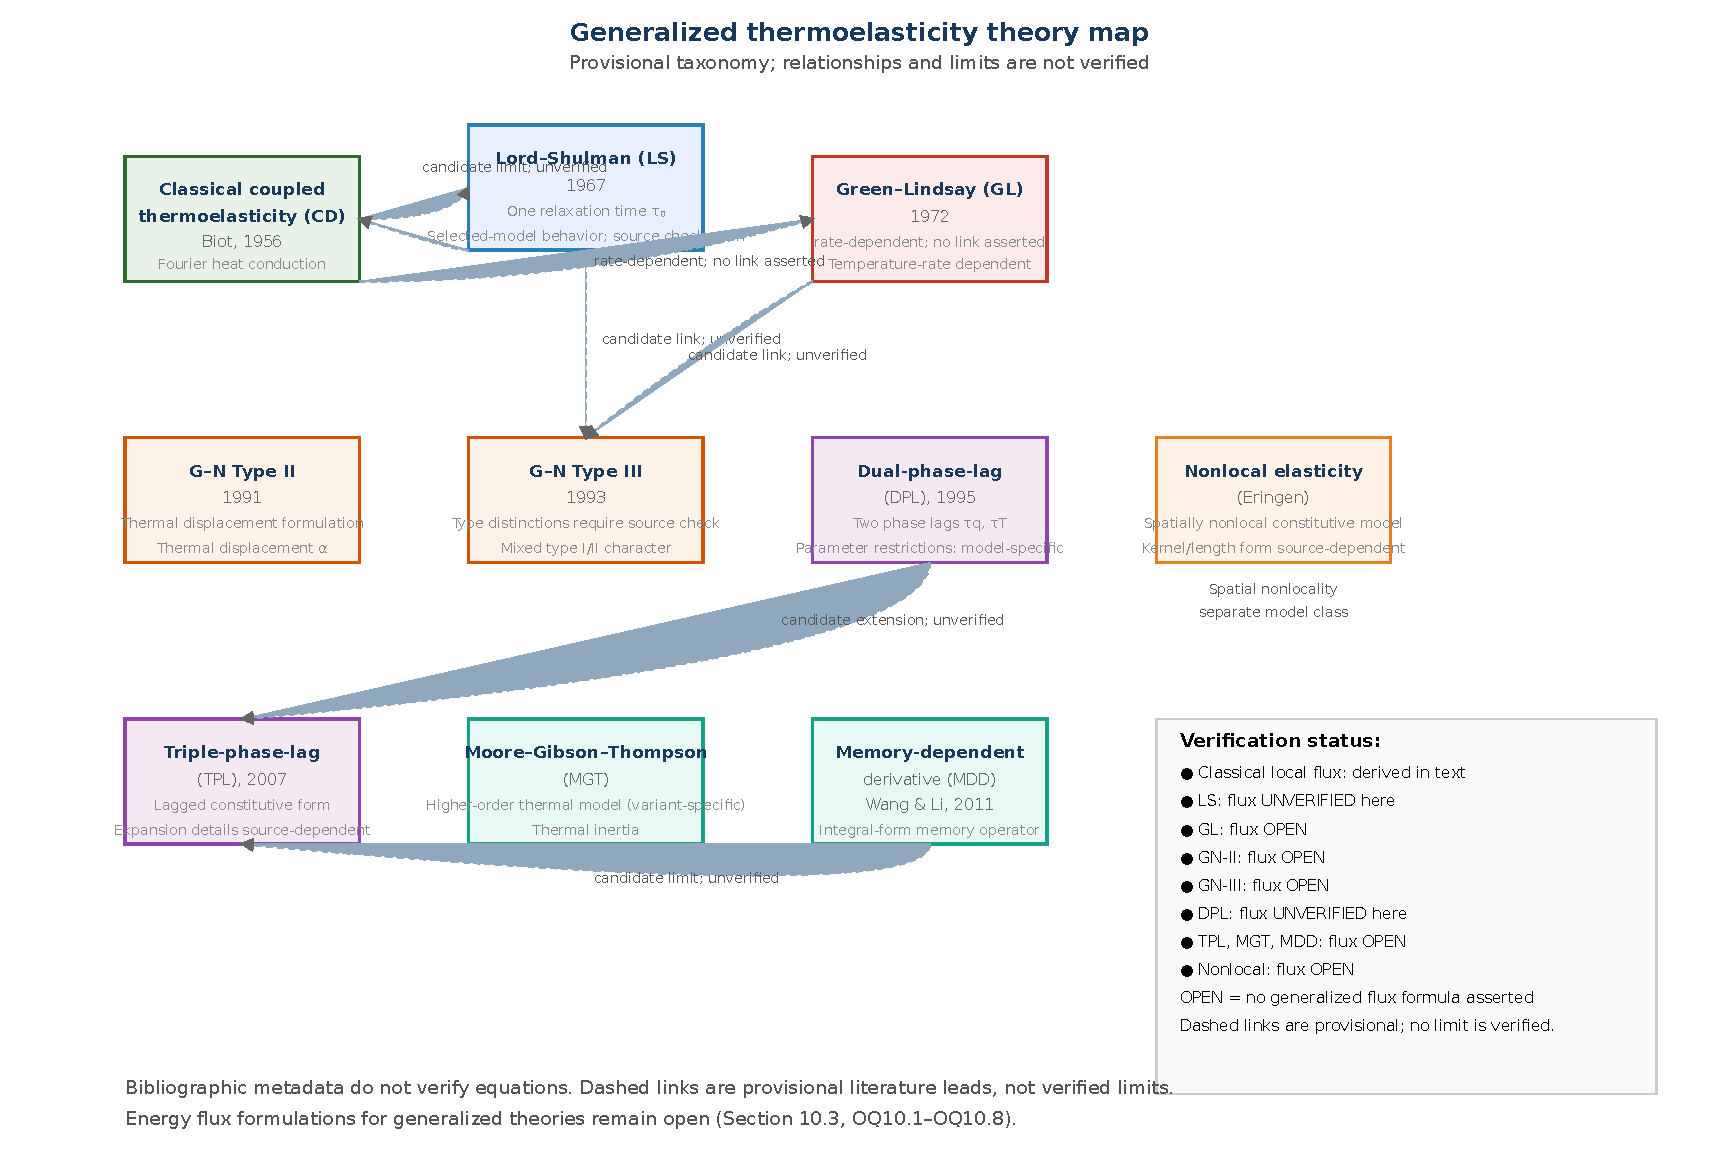
\includegraphics[width=0.95\textwidth]{fig07-theory-map.pdf}
\caption{Schematic map of selected thermoelastic model families. Parameter limits and links are model-specific; no universal reduction or convergence result is asserted. Green--Lindsay is represented as a single-temperature, temperature-rate-dependent theory, distinct from two-temperature models.}
\label{fig:theory_map}
\end{figure}

\subsection{State variables and constitutive distinctions}
\label{sec:4.13}

The model classes surveyed in this section differ in their chosen state variables and constitutive operators. Relaxation models may promote heat flux to an evolving variable; two-temperature formulations distinguish temperature-like fields; thermal-displacement formulations introduce a variable whose time derivative is related to temperature; phase-lag models shift the arguments of constitutive quantities; hereditary and fractional models use history operators. These descriptions are schematic. Their thermodynamic interpretation, initial data, modal consequences, and limiting behavior must be derived from each model's exact equations. In particular, Green--Lindsay is not a two-temperature construction.

\subsection{Thermodynamic admissibility as a selection principle}
\label{sec:4.14}

Thermodynamic admissibility must be established separately for each constitutive family by specifying its free energy, entropy, state variables, evolution laws, and admissible processes. The inherited universal dissipation claims and parameter exclusions have not been re-derived here. No parameter region is excluded, and no Green--Lindsay admissibility result is asserted in this revision without a primary-source derivation.

Thermodynamic restrictions must be derived from the free energy, entropy, heat-flux law, and internal variables of each chosen model. No single dissipation expression or parameter-ordering condition applies to all relaxation, two-temperature, phase-lag, memory-dependent, or fractional formulations. The family-wide assertions in the inherited text are not supported by derivations in this revision and are withdrawn pending model-specific primary-source and thermodynamic checks.

Parameter restrictions are model-specific and must be included when a model is used. The limits and admissible ranges summarized in inherited tables are not treated as verified unless a derivation or full-text source check is identified.

\subsection{Modal structure is model-specific}
\label{sec:4.15}

The modal structure must be obtained by substituting the chosen constitutive equations into the field equations and solving the resulting characteristic problem. A model label alone does not determine the number of propagating, evanescent, or attenuating roots, nor their physical admissibility. The inherited wave-speed, attenuation, and mode-count claims for the relaxation, two-temperature, thermal-displacement, phase-lag, memory-dependent, and fractional families have not been checked in this revision. Root classification and interface matching are therefore treated as problem-specific tasks in Sections~\ref{sec:methods} and~\ref{sec:interfaces}; no universal count or crossover frequency is asserted here.

\subsection{Notation summary for Section 4}

Table \ref{tab:notation-sec4} summarizes the notation introduced in this section.

\begin{table}[htbp]
\centering
\small
\caption{Notation introduced in Section 4.}
\label{tab:notation-sec4}
\begin{tabularx}{\textwidth}{@{}p{1.8cm}X p{2.2cm}p{2.1cm}@{}}
\toprule
\textbf{Symbol} & \textbf{Meaning} & \textbf{Units} & \textbf{Equation} \\
\midrule
$\tau_0$ & LS relaxation time & s & \eqref{eq:4.4} \\
$\tau_q, \tau_T$ & DPL lag parameters in the displayed inherited form & s & \eqref{eq:4.15}--\eqref{eq:4.16} \\
$c_T$ & Thermal wave speed & m/s & \eqref{eq:4.6} \\
$\beta$ & Thermal stress coefficient & Pa/K & \eqref{eq:4.1} \\
$c_v$ & Specific heat at constant strain & J/(kg$\cdot$K) & \eqref{eq:4.2} \\
$k$ & Thermal conductivity & W/(m$\cdot$K) & \eqref{eq:4.2} \\
$\alpha_{\mathrm{GN}}$ & Thermal displacement (GN-II; distinct from fractional order $\alpha$) & K$\cdot$s & \eqref{eq:4.11} \\
$\kappa,\kappa^*$ & GN-III rate and thermal-displacement coefficients & model-dependent & \eqref{eq:4.11}, \eqref{eq:4.14} \\
$p_i$ & Entropy flux (GN-II) & W/(m$^2$$\cdot$K) & \eqref{eq:4.12} \\
$D_{\omega_M}$ & MDD operator & 1/s & \eqref{eq:4.19} \\
$\omega_M$ & MDD finite time horizon & s & \eqref{eq:4.19} \\
$\kappa(t-\xi)$ & MDD kernel & dimensionless & \eqref{eq:4.19} \\
${}^C D_t^\alpha$ & Caputo fractional derivative & $t^{-\alpha}$ & \eqref{eq:4.20} \\
$\alpha$ & Fractional derivative order & dimensionless & \eqref{eq:4.20} \\
$a_\alpha$ & Coefficient in displayed scalar fractional equation & $\mathrm{m^2\,s^{-\alpha}}$ & \eqref{eq:4.20} \\
\bottomrule
\end{tabularx}
\end{table}

\subsection{Open questions for Section 4}

\begin{enumerate}[label=\textbf{OQ4.\arabic*}]
\item What is the complete time-domain energy flux for LS theory, including the contribution from the flux-relaxation term? \\ \label{oq:4.1}
\item What heat-flux law and energy balance follow from the original single-temperature Green--Lindsay relaxation-time convention? \\ \label{oq:4.2}
\item What is the relationship between energy flux and entropy flux in GN-II theory? \\ \label{oq:4.3}
\item What is the mixed energy flux for GN-III theory? \\ \label{oq:4.4}
\item How do different MDD kernel choices affect the energy flux and wave propagation? \\ \label{oq:4.5}
\item Can rigorous limit theorems with convergence proofs be established between theory pairs? \\ \label{oq:4.6}
\end{enumerate}

% LocalWords:


%======================================================================
% Section 5: Coupled Multiphysics Continua
%======================================================================
%======================================================================
% Section 5: Coupled Multiphysics Continua
%======================================================================
\section{Coupled Multiphysics Continua}
\label{sec:multiphysics}

This section surveys coupled continua: piezo-thermoelastic, porous and double-porous, micropolar, semiconductor photo-thermoelastic, and magneto-thermoelastic media. It outlines their governing equations, constitutive relations, coupling mechanisms, and applications; primary sources are cited where available.

\begin{figure}[htbp]
\centering
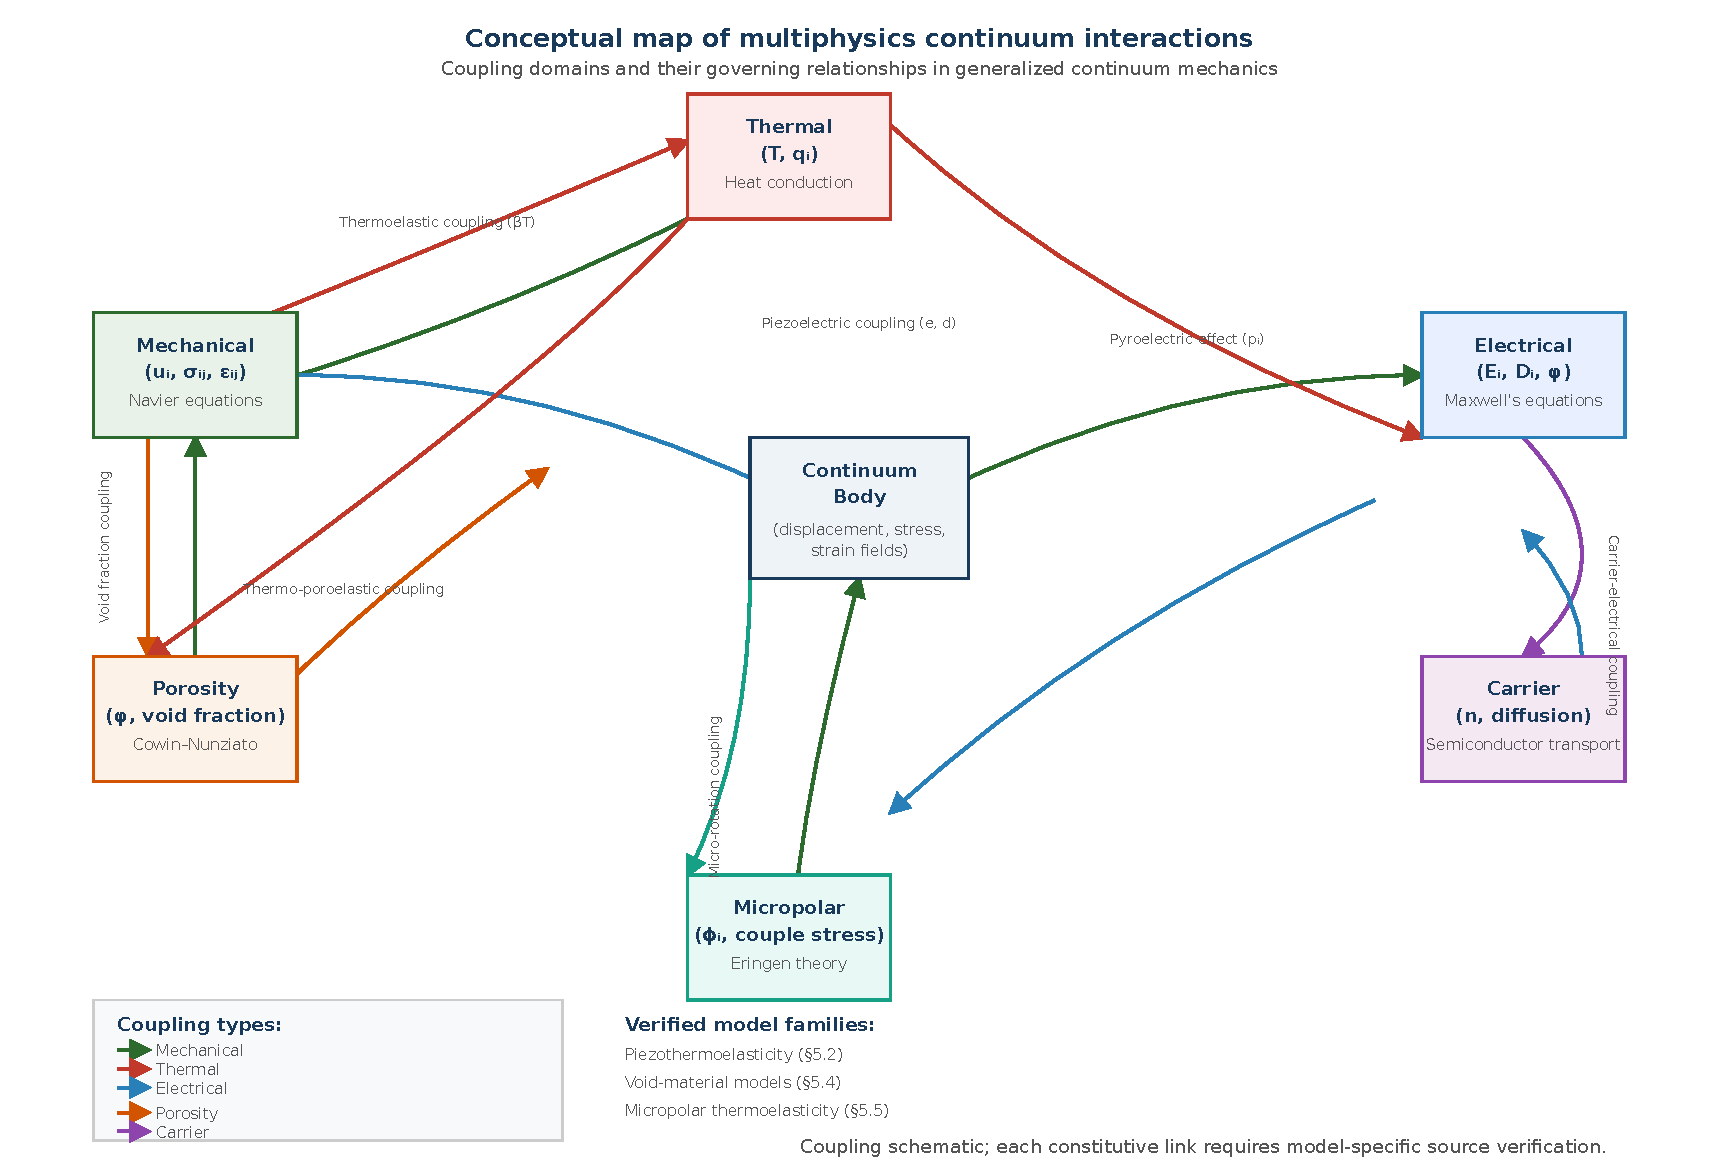
\includegraphics[width=0.95\textwidth]{fig09-multiphysics-coupling.pdf}
\caption{Coupling topology of multiphysics continua. The mechanical field is coupled to a thermal field through the thermoelastic dilatation term, to an electrical field through the piezoelectric tensors, to a porosity field through the void fraction, to a carrier field through the semiconductor transport equations, and to a micro-rotation field through the couple-stress relation. Each coupling is a separate term in a separate equation, and each introduces its own material coefficients and its own additional boundary conditions at an interface; this is the reason that the size of the interface system grows so rapidly as couplings are added (Section~\ref{sec:interfaces}).}
\label{fig:coupling_map}
\end{figure}

\subsection{Piezoelectricity: constitutive relations and coupling coefficients}
\label{sec:5.1}

Piezoelectricity describes the coupling between mechanical and electrical fields in certain crystalline materials (e.g., quartz, barium titanate, lead zirconate titanate). The linear constitutive relations are:

\begin{equation}
\sigma_{ij} = c_{ijkl}\varepsilon_{kl} - e_{kij}E_k,
\label{eq:5.1}
\end{equation}

\begin{equation}
D_i = e_{ikl}\varepsilon_{kl} + \kappa_{ij}E_j,
\label{eq:5.2}
\end{equation}

\begin{equation}
E_i = -\phi_{,i},
\label{eq:5.3}
\end{equation}

where $\sigma_{ij}$ is the Cauchy stress tensor, $c_{ijkl}$ is the elastic stiffness tensor, $\varepsilon_{kl}$ is the infinitesimal strain tensor, $e_{kij}$ is the piezoelectric stress coefficient, $E_k$ is the electric field, $D_i$ is the electric displacement, $\kappa_{ij}$ is the dielectric permittivity, and $\phi$ is the electric potential.

\subsubsection{Charge conservation}

In the absence of free electric charge:

\begin{equation}
D_{i,i} = 0.
\label{eq:5.4}
\end{equation}

\subsubsection{Electrical energy density}

For an uncoupled linear dielectric with symmetric positive-definite permittivity and $D_i=\kappa_{ij}E_j$, the electric-field energy contribution is

\begin{equation}
\mathcal{E}_{\mathrm{elec}} = \frac{1}{2}D_i E_i.
\label{eq:5.5}
\end{equation}

This is not the total stored energy of the coupled piezoelectric system in Eqs.~\eqref{eq:5.1}--\eqref{eq:5.2}; that total requires a stated thermodynamic potential and its mechanical/electrical coupling terms.

\subsection{Piezothermoelasticity: three-field coupling}
\label{sec:5.2}

Piezothermoelasticity couples mechanical, thermal, and electrical fields. The constitutive relations are:

\begin{equation}
\sigma_{ij} = c_{ijkl}\varepsilon_{kl} - e_{kij}E_k - \beta_{ij}T,
\label{eq:5.6}
\end{equation}

\begin{equation}
\sigma_{ij,j} = \rho\ddot{u}_i,
\label{eq:5.7}
\end{equation}

\begin{equation}
E_i = -\phi_{,i},
\label{eq:5.8}
\end{equation}

\begin{equation}
D_i = \kappa_{ij}E_j + e_{ikl}\varepsilon_{kl} + p_i T,
\label{eq:5.9}
\end{equation}

\begin{equation}
D_{i,i} = 0,
\label{eq:5.10}
\end{equation}

where $\beta_{ij}$ is the thermal stress coefficient and $p_i$ is the pyroelectric coefficient.

\subsubsection{Governing equations for coupled fields}

The coupled system consists of the equation of motion \eqref{eq:5.7}, the heat conduction equation (theory-dependent: classical, LS, GL, GN, DPL, TPL, MDD, etc.), and the charge conservation equation \eqref{eq:5.10}. All three fields are coupled through the constitutive relations \eqref{eq:5.6} and \eqref{eq:5.9}: temperature changes induce thermal stresses and pyroelectric effects; mechanical deformation generates piezoelectric polarization; electric fields produce electrostrictive deformation.

\paragraph{Thermopiezoelectric baseline.} On printed pp.~625--626, Mindlin (1974) states the classical three-dimensional linear thermopiezoelectric equations (momentum balance, $D_{i,i}=0$, entropy balance, Fourier heat flux $h_i=-K_{ij}\theta_{,j}$), which are the starting point of his plate reduction, together with linear constitutive equations from an electric Gibbs function \cite{Mindlin1974Thermopiezo}\allowbreak{}.

Generalized piezothermoelastic models may use lagged or memory-dependent heat laws. Mindlin’s Fourier system provides a classical comparison point; each generalized model must be considered with its own equations and parameters.

Coupled thermopiezoelectric formulations combine thermal, mechanical, and electrical fields; their constitutive details depend on the selected model.

Porosity and void fields are additional modeling ingredients; their governing equations and coupling to thermal and electrical fields depend on the selected formulation.

\subsubsection{Modal content of a piezoelectric solid}

The coupling of Section~\ref{sec:5.2} has an immediate and testable consequence: the number of propagating modes increases. A piezoelectric solid admits a quasi-longitudinal mode $qP$, in which the mechanical polarization is essentially parallel to the propagation direction but is accompanied by a longitudinal electric field; a quasi-transverse mode $qS$, whose polarization is essentially transverse but which is accompanied by a transverse electric field whose amplitude is small because the dielectric stiffness dominates; and a quasi-electrostatic potential solution. Under the assumptions used here, $E_i=-\phi_{,i}$ and $D_{i,i}=0$, Maxwell's displacement-current equation is absent; this solution is not an electromagnetic wave and no speed-of-light mode is implied. A propagating electromagnetic branch requires the full Maxwell system and a stated frequency regime.

\subsubsection{The coupling coefficient as a wave-speed diagnostic}

For the displayed linear constitutive equations, eliminating the quasistatic electric field under the open-circuit condition $D_i=0$ gives the effective stiffness
\begin{equation}
\bar{c}_{ijkl} = c_{ijkl} + e_{aij}(\kappa^{-1})_{ab}e_{bkl},
\label{eq:5.19}
\end{equation}
where the positive correction follows from $E_i=-(\kappa^{-1})_{ij}e_{jkl}\varepsilon_{kl}$. Under the short-circuit condition $E_i=0$, the stiffness remains $c_{ijkl}$. The open-circuit correction is positive semidefinite when the permittivity tensor is positive definite and the displayed contractions apply. This is a tensor relation under these electrical constraints, not a universal scalar correction.

\subsection{Electrical boundary conditions}
\label{sec:5.3}

\subsubsection{Perfect electrical contact}

\begin{equation}
\phi^{(1)} = \phi^{(2)} \quad \text{at the interface}.
\label{eq:5.11}
\end{equation}

\subsubsection{Insulated interface}

\begin{equation}
D_i n_i = 0 \quad \text{at the interface}.
\label{eq:5.12}
\end{equation}

\subsubsection{Electric displacement continuity}

\begin{equation}
D_3^{(1)} = D_3^{(2)} \quad \text{at the interface}.
\label{eq:5.13}
\end{equation}

\subsubsection{Why a void needs its own field of freedom}

Void theories do not share one universal field set or balance structure; the source-specific nonlinear, linear-elastic, and thermoelastic formulations below are kept distinct.

\subsubsection{Modal content of a void-bearing medium}

Void-related wave content is source- and model-specific. Cowin and Nunziato's 1983 abstract lists small-amplitude acoustic waves among its applications and states that the deformation-induced change in void volume is determined for those examples (printed p.~125). Iesan's 1986 summary states that acceleration waves are studied for homogeneous, isotropic bodies (printed p.~67). These summaries do not establish a universal fast/slow/shear mode count, which is not assigned here.

\subsection{Porous media: voids and double porosity}
\label{sec:5.4}

The sources distinguish three formulations. Nunziato and Cowin's nonlinear theory describes a void-volume distribution and an admissible thermo-kinetic process; its printed p.~177 balance set includes mass, linear and angular momentum, equilibrated force, energy, and an entropy inequality (Eqs.~(2.7)--(2.12)) \cite{Nunziato1979}. Cowin and Nunziato's separate 1983 linear-elastic theory takes the volume fraction associated with void volume as an independent kinematic variable (printed p.~125, abstract) \cite{Cowin1983}. Iesan's 1986 linear thermoelastic theory uses the deviation $\varphi=v-v_0$ and its gradient alongside strain and temperature variables (printed p.~70, Eqs.~(2.14)--(2.19)) \cite{Iesan1986}.

\subsubsection{Governing equations}

Iesan's 1986 paper gives the following general linear constitutive relations (printed p.~71, Eq.~(2.22)):

\begin{equation}
\begin{aligned}
t_{ij} &= C_{ijrs}e_{rs} + B_{ij}\varphi + D_{ijk}\varphi_{,k} - \beta_{ij}\theta,\\
h_i &= A_{ij}\varphi_{,j} + D_{rsi}e_{rs} + d_i\varphi - a_i\theta,\\
g &= -B_{ij}e_{ij} - \xi\varphi - d_i\varphi_{,i} + m\theta,\\
\rho\eta &= \beta_{ij}e_{ij} + a\theta + m\varphi + a_i\varphi_{,i},\\
q_i &= k_{ij}\theta_{,j}.
\end{aligned}
\label{eq:5.14}
\end{equation}

Here $e_{ij}$ is infinitesimal strain, $\varphi=v-v_0$ is the void-volume deviation, $\theta=T-T_0$ is the temperature increment, $h_i$ is the equilibrated-stress vector, $g$ is the intrinsic equilibrated body force, and $\eta$ is specific entropy. The paper gives a separate isotropic specialization in Eq.~(2.24) and the homogeneous-isotropic field equations in Eq.~(2.28) (printed pp.~71--72); those are not conflated with the general tensor relations above. The 2004 monograph's front-matter contents list chapters on thermoelastic materials with voids and thermoelastic Cosserat continua, with section headings on uniqueness and existence (pp.~v--vi); this is a contents-level description, not a claim about a particular theorem \cite{Iesan2004}.

\subsubsection{Double porosity}

Double porosity models introduce two porosity fields to capture both macro- and micro-porosity effects. The governing equations extend the single-porosity theory with two coupled void volume fractions $\eta_1$ and $\eta_2$, each with its own equilibrated stress and equilibrated body force. Double porosity models are particularly relevant for hydrocarbon reservoirs, fissured rocks, and aquifers where both fracture and matrix porosity contribute to fluid flow and wave propagation.

\subsection{Micropolar and micromorphic continua}
\label{sec:5.5}

Eringen's 1966 paper is titled \emph{Linear Theory of Micropolar Elasticity} \cite{Eringen1966a}; no equation-level claim is made here from the scanned copy. The Tauchert--Claus--Ariman (1968) abstract describes a linear micropolar thermoelastic formulation with displacement/microrotation and stress/couple-stress forms (printed p.~37); its p.~38 notation defines the micro-inertia coefficient $J$ \cite{TauchertClausAriman1968}.

\subsubsection{Governing equations}

Micropolar thermoelastic formulations may include independent microrotation fields and couple stresses. Their constitutive equations depend on the selected kinematics, symmetry assumptions, and thermal coupling.

Micropolar formulations add rotational kinematic and stress measures according to the selected model; the 1968 source is used here only for its stated linear thermoelastic formulation, not for a priority claim or a universal application list.

\subsubsection{The absorption term and the photothermal source}

Illumination does not act on the mechanical field directly; it acts through the heat and the carriers that it generates. The absorbed optical power, attenuated by the Beer--Lambert law, appears as a volumetric source in the thermal equation and as a generation term in the carrier continuity equations. The chain of consequences is then fixed: the thermal source produces a temperature rise; the temperature rise produces a thermoelastic stress through the dilatation term and a pyroelectric polarisation through the pyroelectric coefficient; the stress produces a displacement, and the polarisation produces an electric field, which in turn modifies the carrier distribution. The system is thus closed through the constitutive relations rather than through any additional assumption, and the number of degrees of freedom that must be solved simultaneously is four.

\subsubsection{Photoacoustic waves as a diagnostic of the coupling}

The photoacoustic wave that follows pulsed absorption is the most direct macroscopic observable of the coupling, and it has a distinctive structure: it contains a thermal contribution that propagates at the sound speed, an electronic contribution that propagates at the speed of light but decays on the absorption length, and a thermoelastic contribution whose amplitude depends on the piezoelectric coupling. The relative weight of these contributions depends on the regime --- diffusion-dominated at low frequency, ballistic at high frequency --- and it is the crossover between them that makes the technique sensitive to the thermal model. This is a concrete instance of the general point developed in Section~\ref{sec:applications}: a generalized theory earns its place not by being more general, but by being required in a regime where the classical description demonstrably fails.

\subsection{Semiconductor photo-thermo-elasticity}
\label{sec:5.6}

Semiconductor photo-thermo-elasticity couples mechanical deformation, thermal fields, electrical fields, and carrier density (electrons and holes). When a semiconductor is illuminated, absorbed photons generate electron--hole pairs, producing carrier diffusion, temperature changes, and thermoelastic stresses.

\subsubsection{Governing equations}

The coupled system includes:
\begin{itemize}
\item The equation of motion with piezoelectric and thermal stress terms,
\item The heat conduction equation with carrier recombination heat source,
\item The charge conservation equation with carrier generation and recombination,
\item The carrier continuity equations for electrons and holes.
\end{itemize}

Applications include photoacoustic imaging, semiconductor device thermal management, and optoelectronic sensors.

\subsection{Magneto-thermo-elasticity}
\label{sec:5.7}

Magneto-thermo-elasticity couples mechanical, thermal, and magnetic fields. In electrically conducting media (e.g., liquid metals, plasmas), magnetic fields induce Lorentz forces that couple with thermal stresses.

\subsubsection{Governing equations}

The equation of motion includes the Lorentz force term:

\begin{equation}
\rho\ddot{u}_i = \sigma_{ji,j} + \rho f_i + (\bm{J} \times \bm{B})_i,
\label{eq:5.18}
\end{equation}

where $\bm{J}$ is the current density and $\bm{B}$ is the magnetic flux density.

Applications include magnetohydrodynamic (MHD) systems, liquid metal cooling, geophysical dynamo theory, and electromagnetic forming.

\subsection{Comparative summary}
\label{sec:5.8}

Table \ref{tab:T3-multiphysics} summarizes the coupled multiphysics media: fields, coupling mechanisms, constitutive structure, and applications.

\begin{table}[htbp]
\centering
\small
\caption{Illustrative categories of coupled-field continuum models.}
\label{tab:T3-multiphysics}
\begin{tabularx}{\textwidth}{@{}p{3.2cm}XXXX@{}}
\toprule
\textbf{System} & \textbf{Coupled fields} & \textbf{Governing structure} & \textbf{Constitutive feature} & \textbf{Example source} \\
\midrule
Classical thermoelasticity & Mechanical and thermal & Navier--Fourier system & Thermal-stress coupling; conductivity-based heat equation & \cite{Biot1956} \\
Piezothermo\-elasticity & Mechanical, thermal, and electrical & Coupled piezo--thermal equations & Piezothermal moduli and pyroelectric constants & \cite{Barak2023} \\
Nonlinear elastic materials with voids & Mechanical, void-volume, and entropy fields & Mass, linear/angular momentum, equilibrated-force and energy balances; entropy inequality & Volume distribution; equilibrated stress & \cite{Nunziato1979} \\
Linear elastic materials with voids & Mechanical and void-volume fields & Linear-elastic balance equations & Void fraction is an independent kinematic variable & \cite{Cowin1983} \\
Linear thermoelastic materials with voids & Mechanical, thermal, and void-volume fields & Thermoelastic constitutive restrictions and balances & Void-volume deviation and gradient; temperature and gradient & \cite{Iesan1986} \\
Micropolar thermoelasticity & Mechanical, thermal, and microrotation & Mass, momentum, moment of momentum, energy, and Clausius--Duhem inequality & Couple stress; micro-inertia $J$ & \cite{TauchertClausAriman1968} \\
Semiconductor thermoelectricity & Mechanical, thermal, carrier, and electrical & Carrier transport and heat equations & Carrier and electrical--thermal coupling & Model-specific \\
\bottomrule
\end{tabularx}
\par\smallskip{\footnotesize These categories are illustrative; each coupled system must be specified by its own fields, constitutive equations, and boundary conditions.}
\end{table}


\begin{figure}[htbp]
\centering
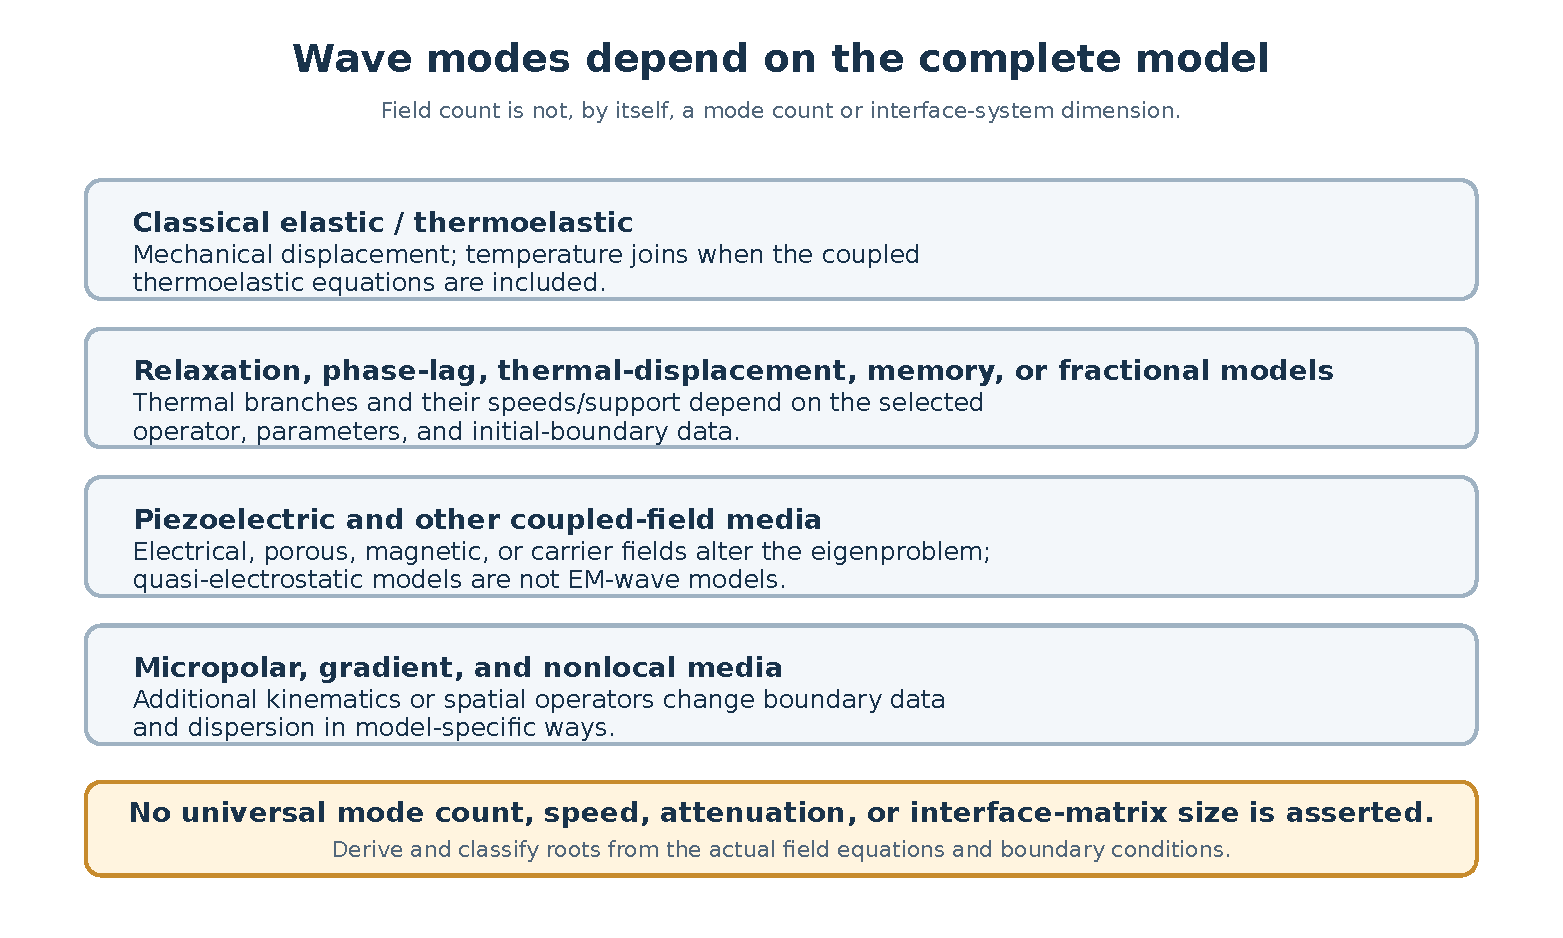
\includegraphics[width=0.9\textwidth]{fig08-wave-types.pdf}
\caption{Schematic overview of field types in continuum wave models. Modal content, propagation, and interface-system dimension depend on the selected constitutive equations and boundary conditions; no universal mode count is asserted.}
\label{fig:wave_types}
\end{figure}

\subsection{The coupling hierarchy and its computational consequences}
\label{sec:5.9}

The number and character of modes and interface conditions depend on the complete field equations, constitutive parameters, geometry, and boundary conditions. An added field or internal variable need not contribute an independent propagating mode, and matrix size is not fixed by a family label.

The secular equation and interface system follow from each model’s field equations and boundary conditions. Their polynomial order and matrix size depend on the selected formulation.

Coupled-field models depend on the free-energy Hessian, constitutive stability, and well-posedness of the initial-boundary-value problem; these properties cannot be inferred from a coupling coefficient alone.

\subsection{Notation summary for Section 5}

\begin{table}[htbp]
\centering
\small
\caption{Notation introduced in Section 5.}
\label{tab:notation-sec5}
\begin{tabularx}{\textwidth}{@{}p{1.8cm}X p{2.2cm}p{2.1cm}@{}}
\toprule
\textbf{Symbol} & \textbf{Meaning} & \textbf{Units} & \textbf{Equation} \\
\midrule
$c_{ijkl}$ & Elastic stiffness tensor & Pa & \eqref{eq:5.1} \\
$e_{kij}$ & Piezoelectric stress coefficient & C/m$^2$ & \eqref{eq:5.1} \\
$\kappa_{ij}$ & Dielectric permittivity & F/m & \eqref{eq:5.2} \\
$E_i$ & Electric field & V/m & \eqref{eq:5.3} \\
$D_i$ & Electric displacement & C/m$^2$ & \eqref{eq:5.2} \\
$\phi$ & Electric potential & V & \eqref{eq:5.3} \\
$\beta_{ij}$ & Thermal stress coefficient & Pa/K & \eqref{eq:5.6} \\
$p_i$ & Pyroelectric coefficient & C/(m$^2$$\cdot$K) & \eqref{eq:5.9} \\
$\bar{c}_{ijkl}$ & Piezoelectrically renormalised stiffness & Pa & \eqref{eq:5.19} \\
$\varphi$ & Void-volume deviation from its reference value (Iesan 1986) & dimensionless & \eqref{eq:5.14} \\
$\eta$ & Specific entropy in Iesan's notation; not the void-volume field & varies & \eqref{eq:5.14} \\
$h_i$ & Equilibrated-stress vector & source-specific & \eqref{eq:5.14} \\
\bottomrule
\end{tabularx}
\end{table}

At the ideal-fluid/nonlocal piezothermoelastic interface studied by Gupta et al., the abstract reports one reflected and four transmitted waves and states that the law of energy conservation across the interface is justified (printed p.~912, abstract). This is an abstract-level report; no exact balance equation is reproduced here \cite{Gupta2023IJNMF}.

A dual-porous thermoelastic interface study reports that the total sum of energy ratios approximates unity; this is retained as a reported numerical observation, not an exact identity \cite{Kumar2023PhysScr}.

\subsection{Open questions for Section 5}

\begin{enumerate}[label=\textbf{OQ5.\arabic*}]
\item What are the complete constitutive relations for piezothermoelastic media with nonlocal elasticity? \\ \label{oq:5.1}
\item How do double-porosity models capture scale-dependent fluid--solid interaction? \\ \label{oq:5.2}
\item What are the energy flux expressions for micropolar media with couple stresses? \\ \label{oq:5.3}
\item How can semiconductor photo-thermo-elastic models be validated experimentally? \\ \label{oq:5.4}
\end{enumerate}

% LocalWords:


%======================================================================
% Section 6: Generalized Transport and Memory Effects
%======================================================================
%======================================================================
% Section 6: Generalized Transport and Memory Effects
%======================================================================
\section{Generalized Transport and Memory Effects}
\label{sec:transport}

Classical Fourier conduction relates heat flux instantaneously to the temperature gradient. Its range of adequacy and any departure from it depend on material, scale, and experiment; no universal failure threshold is asserted here. This section surveys alternative constitutive structures and identifies questions that require model-specific derivation or source checking.

\subsection{Physical origin of thermal relaxation}

Microscopic heat carriers and their scattering can motivate finite-rate transport models, but a continuum relaxation parameter is phenomenological unless it is derived or identified from a specified kinetic model. An exponential relaxation law is one possible constitutive choice, not a universal consequence of carrier dynamics. The memory kernel, relaxation parameters, and resulting wave/support properties must be established for the particular model and material. This section surveys such operator choices while marking family-wide physical interpretations as conditional or unverified.

\subsection{Three structural routes to memory}

Three mathematically distinct ways of making a constitutive law remember have been used, and they are not interchangeable.

\begin{itemize}
\item \textbf{Differential-rate constitutive laws.} Some models include time derivatives of fluxes, temperatures, or other fields; the order and choice of differentiated variable are model-specific. Whether such a law admits an equivalent finite-dimensional internal-variable representation must be established for the particular formulation.
\item \textbf{Integral (convolution) memory.} The constitutive relation is written as a convolution of the driving quantity with a memory kernel over a finite or semi-infinite interval. This includes the hereditary-integral formulation of Section~\ref{sec:transport} and the memory-dependent derivative of Wang and Li \cite{Wang2011}. The memory is then encapsulated in an arbitrary function, and the price is that the constitutive relation is no longer local in time, so that the discretisation must carry the history.
\item \textbf{Spatial nonlocality.} Some constitutive laws average over a material neighbourhood, as in Eringen-type formulations. This is a spatial interaction, not temporal memory, and its operators and boundary conditions require separate treatment in Section~\ref{sec:nonlocal}.
\end{itemize}

\subsection{A transform-domain example, not a universal representation}

Some linear flux laws can be written schematically as
\begin{equation}
\mathcal{D}[\bm{q}] = -k\,\bm{\nabla}T,
\label{eq:6.1}
\end{equation}
but this notation does not make distinct constitutive models equivalent. For the Lord--Shulman/Cattaneo law, with zero initial heat flux,
\begin{equation*}
\bm q+\tau_0\dot{\bm q}=-k\nabla T.
\end{equation*}
The corresponding Laplace-domain multiplier is
\begin{equation}
\mathcal{D}_{\rm LS}(s)=1+\tau_0s.
\label{eq:6.2}
\end{equation}
Nonzero initial flux contributes an additional initial-data term. Fractional, phase-lag, and hereditary models have their own transform symbols and initial terms, which must be derived from their exact constitutive equations; no universal symbol or shared limiting procedure is asserted here.

A comparison in the transform domain is useful only after each constitutive law, initial condition, and admissible parameter range is stated. Formal limits such as $\tau_0\to0$, fractional order tending to an integer, or memory horizon tending to zero require model-specific normalization and convergence arguments. Positivity of a frequency-domain loss modulus, when defined, is not by itself proof of a consistent free energy or a well-posed initial-boundary-value problem. These questions remain model-specific and are not settled uniformly in this review.

\subsection{Fractional operators: Caputo and Riemann--Liouville}
\label{sec:6.2}

Fractional derivatives generalise integer-order differentiation to non-integer orders and are used in models with history dependence. Depending on the operator, coupling, kernel, and initial-boundary conditions, they can produce subdiffusive, dispersive, or wave-like responses. A finite propagation speed or a specific support property is not implied by the fractional order alone.

\subsubsection{Caputo fractional derivative}

The Caputo derivative of order $\alpha$ ($n-1 < \alpha < n$, $n = \lceil\alpha\rceil$):

\begin{equation}
{}^C D_t^\alpha f(t) = \frac{1}{\Gamma(n-\alpha)}\int_0^t \frac{f^{(n)}(\tau)}{(t-\tau)^{\alpha+1-n}}\,d\tau.
\label{eq:6.3}
\end{equation}

\subsubsection{Riemann--Liouville fractional derivative}

\begin{equation}
{}^{RL} D_t^\alpha f(t) = \frac{1}{\Gamma(n-\alpha)}\frac{d^n}{dt^n}\int_0^t \frac{f(\tau)}{(t-\tau)^{\alpha+1-n}}\,d\tau.
\label{eq:6.4}
\end{equation}

For suitable orders and regularity, the Caputo definition uses integer-order initial data, while Riemann--Liouville formulations may involve fractional initial data. This difference can matter in model selection, but it does not establish a universal preference. The historical motivations and material interpretations attributed to fractional operators require claim-level source checking; the citations here are source leads, not independently verified support for those claims.

\subsubsection{Fractional heat conduction and its limits}

\begin{equation}
{}^C D_t^\alpha T = a_\alpha\nabla^2 T, \qquad 0 < \alpha \leq 2,
\label{eq:6.5}
\end{equation}
Here $a_\alpha$ is a model coefficient with dimensions consistent with the selected order (for length and time units, $[a_\alpha]=L^2T^{-\alpha}$). This scalar equation is illustrative, not a universal fractional thermoelastic law. At the integer-order endpoints, the corresponding scalar PDE has heat-equation or wave-equation form, with coefficients and initial data specified for each model; one cannot infer a common dimensional parameter or solution limit across orders. Intermediate-order propagation and well-posedness depend on the operator definition, coupling, domain, and data. The cited Povstenko papers are relevant source leads for fractional thermoelasticity, but no theorem or material interpretation from them has been checked in full text in this revision.

\subsection{Hereditary integrals: convolution kernels}
\label{sec:6.3}

One common representation of linear temporal memory is a hereditary integral:

\begin{equation}
f(t) = \int_{-\infty}^{t} K(t-\xi)\,g(\xi)\,d\xi,
\label{eq:6.6}
\end{equation}
where $K(t-\xi)$ is a kernel in this schematic convolution. Some models impose fading-memory, positivity, monotonicity, or complete-monotonicity hypotheses, but the required conditions depend on the constitutive law and the chosen thermodynamic framework; none of these properties alone is asserted here as a universal admissibility criterion. For suitable completely monotone kernels, representation results by weighted exponentials may apply, but their hypotheses and implications must be checked for the kernel at hand. No equivalence with a discrete phase-lag hierarchy is claimed.

\subsection{Memory-dependent derivative (MDD): operator and kernel}
\label{sec:6.4}

An operator attributed to Wang and Li \cite{Wang2011} uses a kernel over a finite interval. The exact definition and its relation to other memory models remain subject to primary-source checking:

\begin{equation}
D_\omega f(t) = \frac{1}{\omega}\int_{t-\omega}^{t} \kappa(t-\xi) f'(\xi)\,d\xi,
\label{eq:6.7}
\end{equation}
where $\omega>0$ denotes the displayed horizon and $\kappa$ is the kernel. The bounds, normalization, regularity, and admissibility conditions on $\kappa$ must be taken from the exact model definition. A finite integration horizon truncates the history in this formula; it does not by itself imply a finite-dimensional state-space realization, finite computation cost, or that the kernel is a freely chosen rather than material-calibrated quantity.

\subsubsection{MDD kernel function}

A commonly used kernel is
\begin{equation}
\kappa(t-\xi) = 1 - \frac{2\beta}{\omega}(t-\xi) + \frac{\alpha^2}{\omega^2}(t-\xi)^2,
\label{eq:6.8}
\end{equation}
where $\alpha$ and $\beta$ are parameters in this inherited candidate kernel. Its dimensions, bounds, normalization, and any admissible parameter region require checking against the defining source and the selected thermodynamic model; positivity or monotonicity alone is not taken as a proof of admissibility.

\subsubsection{Limiting behavior}

A formal short-horizon limit $\omega\to0$ is often used to recover an ordinary derivative from a normalized finite-horizon operator. The displayed kernel normalization and regularity assumptions must be specified before this limit is asserted; it is retained as a candidate limiting relation and is not used as a proven model equivalence. No exact exponential-kernel reduction to Lord--Shulman, or general equivalence with a fractional operator, is asserted here.

\subsection{Energy flux in memory-dependent media}
\label{sec:6.5}

A candidate outward-positive local flux for a classical mechanical balance with a specified heat-flux vector is
\begin{equation}
J_i(t) = q_i(t)-\sigma_{ij}(t)v_j(t).
\label{eq:6.10}
\end{equation}
This is not asserted as a complete total-energy flux for every memory-dependent theory. The MDD heat-flux law and the appropriate stored-energy/boundary-power terms must be derived together from the selected kernel and free energy. The subsequent equations are inherited candidate constitutive forms, not independently source-checked here:
\begin{equation}
q_i(t) + \tau_0 D_\omega q_i(t) = -k T_{,i}(t),
\label{eq:6.11}
\end{equation}
\begin{equation}
q_i(t) + \frac{\tau_0}{\omega}\int_{t-\omega}^{t} \kappa(t-\xi) \dot{q}_i(\xi)\,d\xi = -k T_{,i}(t).
\label{eq:6.12}
\end{equation}
No universal hereditary correction to the energy flux, or generalized local balance, is asserted. Status of Eqs.~\eqref{eq:6.11}--\eqref{eq:6.12} and the corresponding MDD free-energy balance: UNVERIFIED / OPEN pending primary-source and derivation audit.

\subsection{Well-posedness and propagation in memory-dependent models}
\label{sec:6.6}

Well-posedness and propagation depend on the exact memory operator, kernel, time horizon, initial data, domain, and boundary conditions. Positivity or monotonicity of a kernel alone is not a general sufficient proof of a well-posed initial-boundary-value problem. Likewise, a finite-horizon derivative does not by itself imply finite propagation speed. The inherited claims about universal admissibility restrictions, a Banach-space existence theorem, and finite thermal-wave speed have not been independently verified and are not asserted as results in this revision. A model-specific energy estimate and existence/uniqueness analysis are OPEN.

\subsection{Comparative summary: transport models}

Table \ref{tab:transport_comparison} summarizes transport and memory models across mathematical structure, dissipation, well-posedness, and energy flux status.

\begin{table}[htbp]
\centering
\small
\caption{Provisional transport-family comparison. Entries for generalized models are audit questions, not verified admissibility or well-posedness results.}
\label{tab:transport_comparison}
\begin{tabularx}{\textwidth}{@{}p{2.4cm}XXX@{}}
\toprule
\textbf{Model class} & \textbf{Transport structure} & \textbf{Energy/admissibility status here} & \textbf{Evidence status} \\
\midrule
Classical Fourier & Local Fourier heat flux & Classical local balance derived; Fourier heat equation parabolic & DERIVED / standard model \\
Lord--Shulman & Relaxing heat flux & Model-specific free energy, dissipation and initial data not checked & OPEN \\
Green--Lindsay & Temperature-rate-dependent formulation & Single-temperature description; source-level equations and admissibility not checked & UNVERIFIED \\
Phase-lag (dual/triple) & Lagged constitutive laws & Restrictions and stability depend on selected truncation and parameter set & OPEN \\
Green--Naghdi II/III & Thermal-displacement formulations & Family-specific energy and dissipation identities not checked & OPEN \\
Moore--Gibson--Thompson & Higher-order heat equation variants & Stability and admissibility not checked here & OPEN \\
Memory-dependent & Kernel/time-history operator & Kernel-specific balance and well-posedness not checked & OPEN \\
Fractional & Fractional time operator & Propagation and admissibility depend on operator and data space & OPEN \\
Nonlocal / gradient & Spatially nonlocal or higher-gradient law & Boundary power and domain-specific balance not derived & OPEN \\
\bottomrule
\end{tabularx}
\end{table}

\begin{figure}[htbp]
\centering
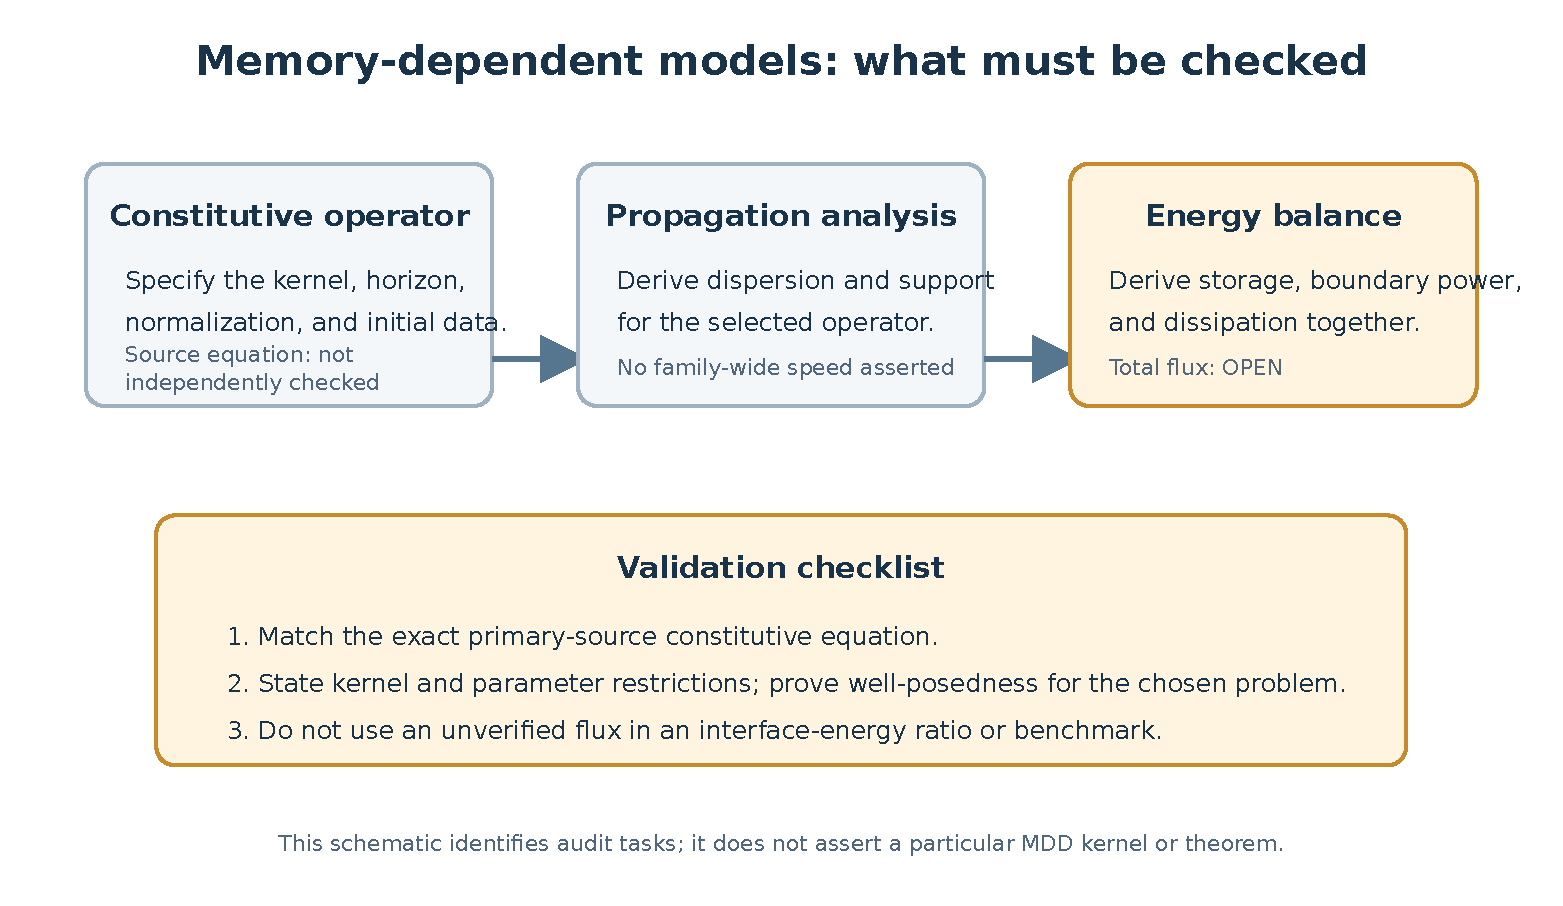
\includegraphics[width=0.95\textwidth]{fig10-mdd-memory.pdf}
\caption{Schematic of a finite-horizon memory-dependent operator and audit questions concerning its kernel, limiting behavior, energy balance, and well-posedness. Model-specific propagation and flux consequences are not asserted; the displayed operator remains subject to primary-source verification.}
\label{fig:mdd_memory}
\end{figure}

\subsection{Notation summary for Section 6}

\begin{table}[htbp]
\centering
\small
\caption{Notation introduced in Section 6.}
\label{tab:notation-sec6}
\begin{tabularx}{\textwidth}{@{}p{1.8cm}X p{2.2cm}p{2.1cm}@{}}
\toprule
\textbf{Symbol} & \textbf{Meaning} & \textbf{Units} & \textbf{Equation} \\
\midrule
$\mathcal{D}[\cdot]$ & Generic memory operator acting on the flux & --- & \eqref{eq:6.1} \\
$\mathcal{D}_{\rm LS}(s)$ & LS transform multiplier (zero initial flux) & dimensionless & \eqref{eq:6.2} \\
${}^C D_t^\alpha$ & Caputo fractional derivative & $t^{-\alpha}$ & \eqref{eq:6.3} \\
${}^{RL} D_t^\alpha$ & Riemann--Liouville derivative & $t^{-\alpha}$ & \eqref{eq:6.4} \\
$a$ & Thermal diffusivity & m$^2$/s & \eqref{eq:6.5} \\
$K(t-\xi)$ & Memory kernel & varies & \eqref{eq:6.6} \\
$D_\omega$ & MDD operator & 1/s & \eqref{eq:6.7} \\
$\omega$ & MDD time delay (horizon) & s & \eqref{eq:6.7} \\
$\kappa(t-\xi)$ & MDD kernel & dimensionless & \eqref{eq:6.8} \\
$\alpha, \beta$ & MDD kernel parameters & varies & \eqref{eq:6.8} \\
$\tilde{q}_i(s)$ & Laplace transform of the heat flux & --- & \eqref{eq:6.2} \\
\bottomrule
\end{tabularx}
\end{table}

\subsection{Open questions for Section 6}

\begin{enumerate}[label=\textbf{OQ6.\arabic*}]
\item What is the complete time-domain energy flux for MDD media with convolution-type memory, expressed solely in terms of the temperature and the stored internal variables? \\ \label{oq:6.1}
\item How is energy partitioned between storage and dissipation in hereditary media, and what is the correct effective flux that enters a local balance? \\ \label{oq:6.2}
\item What are the well-posedness conditions for fractional-order thermoelasticity with arbitrary $\alpha$, in the coupled mechanical setting rather than in isolation? \\ \label{oq:6.3}
\item How do different MDD kernel choices affect the energy flux and the wave propagation, and can the dispersion of the thermal branch be used to identify the kernel experimentally? \\ \label{oq:6.4}
\item Can the memory operator be given a finite-dimensional state-space realisation for a general admissible kernel, and what is the numerical cost of that realisation relative to a direct quadrature? \\ \label{oq:6.5}
\end{enumerate}

% LocalWords:


%======================================================================
% Section 7: Nonlocal and Scale-Dependent Continuum Models
%======================================================================
%======================================================================
% Section 7: Nonlocal and Scale-Dependent Continuum Models
%======================================================================
\section{Nonlocal and Scale-Dependent Continuum Models}
\label{sec:nonlocal}

Many classical local constitutive models relate stress to strain at the same material point and contain no explicit internal length. Nonlocal, gradient, couple-stress, and micropolar models introduce spatial interactions or additional kinematics to represent possible size effects. Their use is motivated by particular materials and experiments; evidence of a characteristic microstructural scale does not by itself show that a classical local law is invalid in every small-scale regime. The applicable constitutive model and its length parameter require independent justification.

This section develops that class. The organising question is not which of the competing formulations is correct, but \emph{which physical mechanism each one encodes}, because the mechanisms predict measurably different dispersion and therefore admit different experimental tests.

\subsection{Physical motivation and constitutive foundations}
\label{sec:7.1}

The classical assumption fails in a specific and observable way. A beam of a given material, tested in bending, exhibits a stiffness that depends on the specimen thickness: thinner specimens are stiffer than the classical prediction, and the departure becomes significant below a material-dependent critical length. Two distinct physical mechanisms can produce this behaviour, and they are the root of the entire family of models considered here.

The first mechanism is \emph{constitutive}: the internal stress in the material depends on the neighbouring material state, because the mechanism that carries load---bonding, dislocation motion, stress concentration in a heterogeneous microstructure---acts over a finite distance. Eringen's formulation of nonlocal elasticity is the canonical statement of this mechanism \cite{Eringen1972,Eringen1974}, in which the stress at a point is obtained by averaging the local stress over a neighbourhood weighted by a kernel:

\begin{equation}
\sigma_{ij}(\bm{x}) = \int_\Omega \alpha(|\bm{x}' - \bm{x}|, \tau)\, \sigma_{ij}^{\mathrm{local}}(\bm{x}')\, d\Omega_{\bm{x}'},
\label{eq:7.1}
\end{equation}
where $\alpha$ is the attenuation kernel and $\tau = e_0 a/\ell$ is the nonlocal parameter, with $e_0$ a material constant, $a$ an internal characteristic length such as the lattice spacing, and $\ell$ an external characteristic length such as the specimen size. The nonlocal parameter is therefore not an arbitrary length: it is a ratio of an internal to an external scale, which means that the nonlocal correction grows in relative importance as the specimen is made smaller relative to the microstructure. This is the scaling property that distinguishes a size-dependent theory from an ad hoc correction.

The second mechanism is \emph{structural}: the material possesses additional internal degrees of freedom---microrotations, relative displacement of the constituents of a porous skeleton, dislocation density---whose motion must be carried by additional stress measures. Micropolar elasticity, formulated by Eringen as a linear theory of a continuum with independent microrotation fields \cite{Eringen1966a} and extended to the thermoelastic case by Tauchert, Claus and Ariman \cite{Eringen1968b}, is the earliest and most complete statement of this mechanism. Later work extended it to materials with voids, in which the skeleton and the pore fluid carry independent kinematic fields \cite{Nunziato1979,Cowin1983}, with a corresponding thermoelastic formulation \cite{Iesan1986}.

\subsubsection{Differential form}

For special kernel functions---notably the one-parameter exponential and the Helmholtz kernel---the integral equation of Eq.~\eqref{eq:7.1} reduces to a differential equation of higher order. For the Helmholtz kernel one obtains

\begin{equation}
(1 - \xi^2\nabla^2)\sigma_{ij} = \sigma_{ij}^{\mathrm{local}},
\label{eq:7.2}
\end{equation}
where $\xi = e_0 a$ is the nonlocal length scale parameter. The differential form is the one used in wave-propagation applications, because it is a partial differential equation and can therefore be treated with the transform and numerical machinery of Section~\ref{sec:methods}. It is worth recording that the differential and integral forms are not interchangeable in general: the integral relation with a given kernel and the differential operator of Eq.~\eqref{eq:7.2} agree only for that kernel, and the difference matters for the boundary conditions, which in the differential form become higher-order \cite{Polizzotto2001}.

\subsection{Strain-gradient and couple-stress theories}
\label{sec:7.2}

Strain-gradient theory extends classical elasticity by including higher-order gradients of strain in the constitutive relations:

\begin{equation}
\sigma_{ij} = C_{ijkl}\varepsilon_{kl} - \ell^2 C_{ijkl}\nabla^2\varepsilon_{kl},
\label{eq:7.3}
\end{equation}

where $\ell$ is a material length scale parameter. The physical reading of Eq.~\eqref{eq:7.3} is that the stress depends not only on the strain but on the curvature of the strain field, so that regions in which the strain varies rapidly---near a notch, a contact edge, or an interface---carry additional stress. The coefficient $\ell$ is a genuine material constant that must be measured; the identification procedures for it, together with the finite element implementations and the variational formulations that make the theory tractable, have been surveyed by Askes and Aifantis \cite{Askes2006,Askes2011}.

The unifying point of view that connects gradient elasticity to micropolar and couple-stress elasticity is that all three introduce internal degrees of freedom and a length scale, and differ in whether those degrees of freedom are constrained to coincide with the macroscopic deformation or are allowed to evolve independently. Aifantis's formulation, in which the internal length is interpreted as the scale of the microstructural heterogeneity that generates it, is the common root \cite{Askes2006}. It follows that a continuum model with internal length, in whichever of these forms, can be used to represent materials for which no explicit microstructural model is available---which is why the same length-scale parameter appears in treatments of metals, polymers, granular media, and biological tissue with broadly comparable values.

\subsection{Size-dependent wave behavior: dispersion from nonlocality}
\label{sec:7.3}

Nonlocality introduces dispersion: the wave speed depends on wavelength. The differential form of nonlocal elasticity was developed by Eringen \cite{Eringen1983}, and the size-dependent elastic effects at the nanoscale were quantified by Maranganti and Sharma \cite{Maranganti2007}, who established the characteristic length below which classical elasticity fails for a range of materials, and by Maranganti, Sharma and Sharma \cite{Maranganti2006}, who showed that the nanoscale nonlocal contribution to electromechanical coupling is generically non-zero even for materials that possess no piezoelectric tensor---a result directly relevant to the coupled theories of Section~\ref{sec:multiphysics}, because it means that a purely elastic size effect can generate an apparent electromechanical response in a nominally non-piezoelectric material.

For a nonlocal elastic bar, the dispersion relation is

\begin{equation}
c(k_{\mathrm w}) = \frac{c_0}{\sqrt{1 + \xi^2 k_{\mathrm w}^2}},
\label{eq:7.4}
\end{equation}

where $c_0$ is the classical wave speed, $k_{\mathrm w}$ is the wave number (distinct from the thermal conductivity $k$), and $\xi$ is the nonlocal length scale. Long waves ($k_{\mathrm w} \to 0$) approach the classical speed $c_0$; short waves are strongly slowed.

\subsubsection{The dispersion signature distinguishes the mechanisms}

For Eq.~\eqref{eq:7.4}, the phase speed tends to zero as $k_{\mathrm w}\to\infty$, while the angular frequency $\omega(k_{\mathrm w})=c_0 k_{\mathrm w}/\sqrt{1+\xi^2k_{\mathrm w}^2}$ approaches the finite limit $c_0/\xi$; it is frequency, not phase speed, that saturates. The group velocity is $d\omega/dk_{\mathrm w}=c_0(1+\xi^2k_{\mathrm w}^2)^{-3/2}$ and tends to zero. By contrast, the positive strain-gradient law in Eq.~\eqref{eq:7.3} gives $c_{\rm ph}^2=c_0^2(1+\ell^2 k_{\mathrm w}^2)$ for a one-dimensional bar, so it stiffens and phase speed increases. Gradient-inertia variants can behave differently; the model form must accompany any comparison. A dispersion measurement over a sufficiently broad range of $k_{\mathrm w}$ can thus distinguish a nonlocal mechanism from a gradient mechanism, and the two are not interchangeable even though both produce the same qualitative signature of a size-dependent stiffness. This is one of the few places in the reviewed literature where two competing formulations of the same effect make quantitatively different and testable predictions, and it deserves more attention than it has received.

\begin{figure}[htbp]
\centering
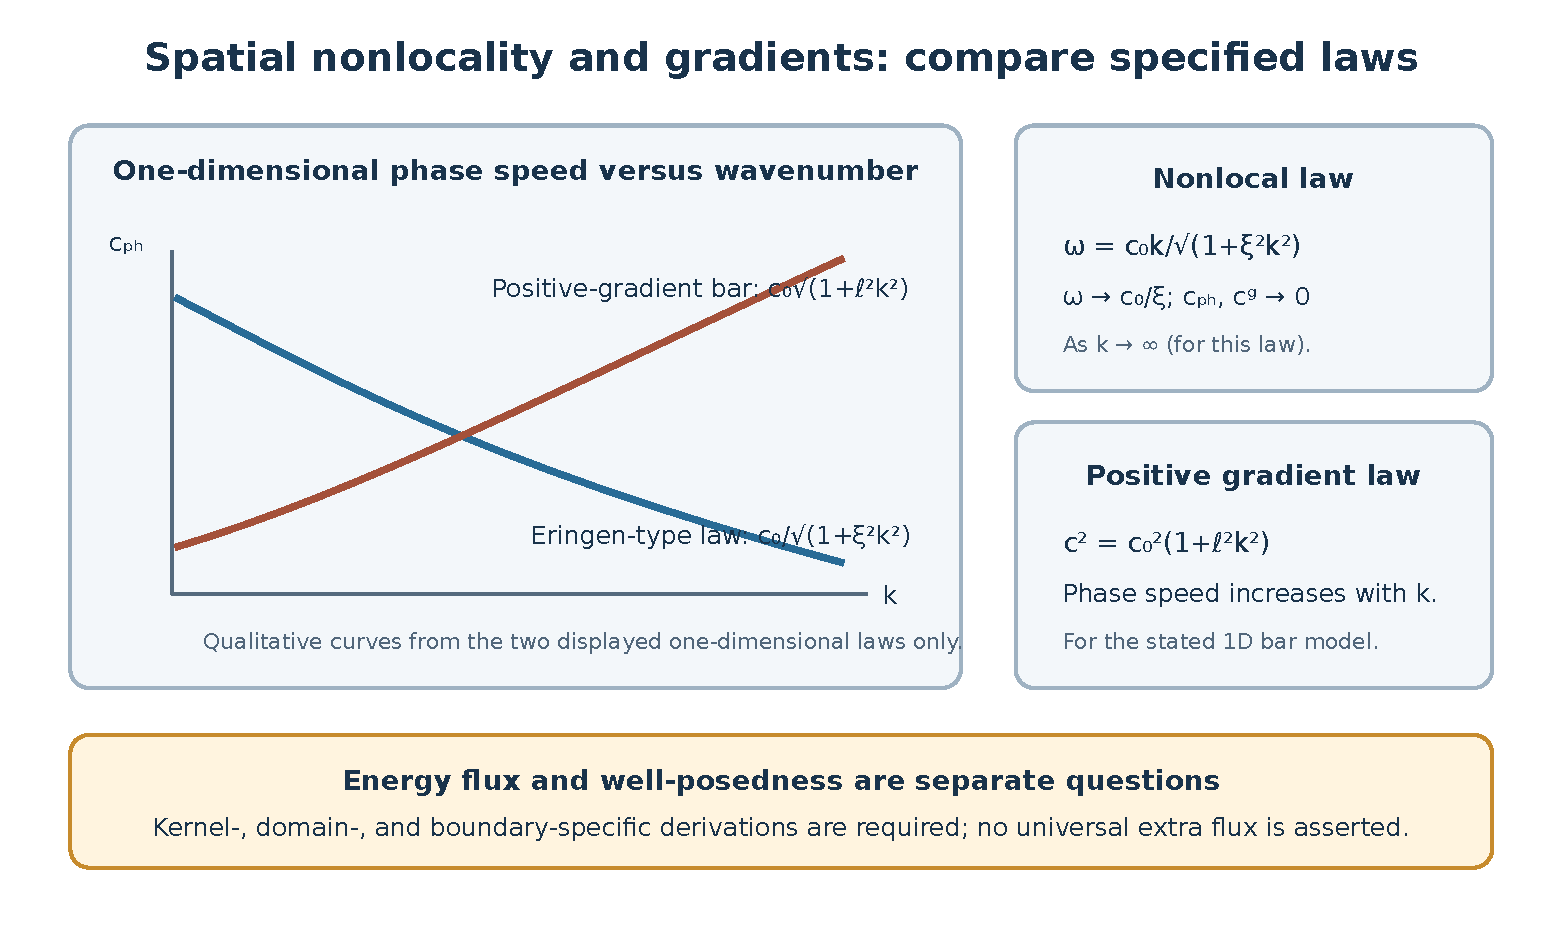
\includegraphics[width=0.95\textwidth]{fig11-nonlocality.pdf}
\caption{Schematic nonlocal and gradient mechanisms. The plotted dispersion curves correspond only to the particular one-dimensional laws stated in Section 7; other gradient-inertia or kernel choices can differ. No universal nonlocal energy-flux correction is asserted; boundary-power derivations remain open.}
\label{fig:nonlocality}
\end{figure}

\subsection{Energy flux in nonlocal media}
\label{sec:7.4}

For nonlocal media, boundary-power terms depend on the kernel, domain, constitutive free energy, and boundary conditions. A flux identity for a given model must be derived from its power balance; no universal correction is assumed.

\subsection{Interface conditions for nonlocal media}
\label{sec:7.5}

Interface conditions for nonlocal media differ from the classical ones because the stress at a point depends on the strain in a neighbourhood, and a neighbourhood straddling an interface samples both media. The classical conditions---continuity of displacement and of traction---must be supplemented, and the supplementation is not unique: one may impose conditions on the additional derivatives that appear in the differential form of Eq.~\eqref{eq:7.2}, or one may impose the conditions in the integral form by requiring the nonlocal stress to be continuous across the interface. The two are not equivalent, and the choice made determines the number and kind of boundary conditions that the resulting boundary-value problem admits. For the differential form, the interface conditions include both the classical conditions and the higher-order conditions arising from the $\nabla^2$ term.

Interface problems in which the nonlocal operator is combined with an additional coupled field have been analysed in the reviewed corpus for a fluid in contact with a nonlocal piezothermoelastic medium \cite{Gupta2023IJNMF} and for nonlocal Kelvin--Voigt piezo-semiconductors under a memory-dependent heat flux \cite{Gupta2026HeatMap}. In both cases the analysis proceeds through the modal machinery of Section~\ref{sec:interfaces}, and the specific difficulty in both is the same: the nonlocal operator acts on the stress while the coupled field acts on the temperature or the electric displacement, and the interface conditions must be formulated consistently for both.

\subsection{What nonlocality does not repair}
\label{sec:7.6}

The differential nonlocal model must be distinguished from the integral constitutive law from which it is sometimes obtained. Its boundary-value formulation can exhibit paradoxes under particular geometries and boundary conditions, including the cantilever-bending paradox discussed in the nonlocal-beam literature; that does not establish a bulk-wave group velocity that grows without bound. For Eq.~\eqref{eq:7.4}, both frequency and group velocity are bounded. Well-posedness claims must specify operator, domain, boundary conditions and function space; no universal Hadamard-instability claim is made here.

Some nonlocal formulations exhibit boundary-value paradoxes for particular kernels, geometries, or boundary conditions. Bounded kernels and variational formulations have been proposed in parts of the literature, but their ability to resolve a given problem must be demonstrated for the specified operator and function space; neither is a universal remedy or proof of well-posedness. The variational route can clarify admissible boundary data, but its conclusions are model-specific.

\subsection{Comparative summary: nonlocal models}

\begin{table}[htbp]
\centering
\small
\caption{Model-specific comparison of spatially nonlocal and gradient formulations. Dispersion statements are restricted to the one-dimensional laws displayed in this section.}
\label{tab:nonlocal_comparison}
\begin{tabularx}{\textwidth}{@{}p{2.4cm}XXX@{}}
\toprule
\textbf{Model/form used here} & \textbf{Spatial mechanism} & \textbf{Dispersion feature} & \textbf{Energy/flux terms to specify} \\
\midrule
Eringen-type Helmholtz form, Eq.~\eqref{eq:7.2} & Kernel-dependent spatial averaging & One-dimensional result of Eq.~\eqref{eq:7.4}; phase speed decreases and frequency tends to $c_0/\xi$ & Flux depends on the specified kernel and boundary-value problem \\
Strain-gradient form, Eq.~\eqref{eq:7.3} & Strain-curvature term & For the stated positive-gradient 1D bar, phase speed increases with $k_{\mathrm w}$ & Higher-gradient boundary power depends on additional boundary data \\
Micropolar / couple-stress & Additional micro-rotation or couple stress & Depends on the selected micropolar model & Model-specific flux terms \\
Two-phase local/nonlocal & Depends on selected mixture/kernel & Depends on the selected mixture/kernel & Model-specific flux terms \\
\bottomrule
\end{tabularx}
\end{table}

\subsection{Notation summary for Section 7}

\begin{table}[htbp]
\centering
\small
\caption{Notation introduced in Section 7.}
\label{tab:notation-sec7}
\begin{tabularx}{\textwidth}{@{}p{1.8cm}X p{2.2cm}p{2.1cm}@{}}
\toprule
\textbf{Symbol} & \textbf{Meaning} & \textbf{Units} & \textbf{Equation} \\
\midrule
$\alpha(|\bm{x}'-\bm{x}|,\tau)$ & Nonlocal attenuation kernel & varies & \eqref{eq:7.1} \\
$\tau$ & Nonlocal parameter, ratio of internal to external length & dimensionless & \eqref{eq:7.1} \\
$e_0$ & Material constant of the nonlocal formulation & dimensionless & \eqref{eq:7.1} \\
$a$ & Internal characteristic length & m & \eqref{eq:7.1} \\
$\xi = e_0 a$ & Nonlocal length scale parameter & m & \eqref{eq:7.2} \\
$\ell$ & Strain-gradient or couple-stress length scale & m & \eqref{eq:7.3} \\
$k_{\mathrm w}$ & One-dimensional wave number & m$^{-1}$ & \eqref{eq:7.4} \\
$c(k_{\mathrm w})$ & Wave speed as a function of wave number & m\,s$^{-1}$ & \eqref{eq:7.4} \\
$c_0$ & Classical (local) wave speed & m\,s$^{-1}$ & \eqref{eq:7.4} \\
\bottomrule
\end{tabularx}
\end{table}

These examples show that nonlocal operator placement is model-specific. Lata and Singh's two-temperature nonlocal thermoelastic model uses a conductivity-based heat equation, with no phase-lag or Green–Naghdi term in the stated formulation. \cite{Lata2020}. Gupta et al.'s nonlocal fractional MGT example places the spatial operator in its constitutive relations, inertial term, and heat-flux relation; the latter includes temperature- and thermal-displacement-gradient terms and a carrier contribution. \cite{Gupta2024}. For one modified-Bessel $K_0$ attenuation kernel, Li and He give a kernel-specific correspondence with a differential nonlocal relation. \cite{Li2018}. A separate cited study treats Klein–Gordon-type nonlocal elasticity in wave propagation; no operator-placement detail is inferred here. \cite{Lazar2022}. Tung's nonlocal piezoelastic half-space model applies a spatial operator to the stress and electric-displacement relations, with a corresponding factor in the motion equation; no heat equation is included. \cite{Tung2019}. In Zang et al.'s one-dimensional piezoelectric nanoplate model, scale-dependent terms enter the inertia contributions; the study examines longitudinal-wave dispersion with surface effects. \cite{Zang2014}.

\subsection{Open questions for Section 7}

\begin{enumerate}[label=\textbf{OQ7.\arabic*}]
\item What is the correct energy flux at a nonlocal interface, derived from a rigorous modified divergence theorem, and does it reproduce the classical limit as $\xi \to 0$? \label{oq:7.1}
\item How must the boundary conditions be formulated for the differential nonlocal operator so that the initial-value problem is well posed, and is the resulting formulation variational? \label{oq:7.2}
\item What is the relationship between the integral and differential nonlocal formulations at the level of the energy flux, given that the two agree only for the specific kernel used to obtain the differential form? \label{oq:7.3}
\item Can a dispersion measurement over a sufficiently broad range of wave number distinguish a nonlocal mechanism from a gradient mechanism in a specific material? \label{oq:7.4}
\item Which nonlocal constitutive law is thermodynamically admissible when combined with a memory-dependent thermal law, given that both introduce history into the energy balance? \label{oq:7.5}
\end{enumerate}

% LocalWords:


%======================================================================
% Section 8: Mathematical Methods for Wave Propagation
%======================================================================
%======================================================================
% Section 8: Mathematical Methods for Wave Propagation
%======================================================================
\section{Mathematical Methods for Wave Propagation}
\label{sec:methods}

The theory families considered here differ in constitutive assumptions and governing equations. Several analytical tools---plane-wave ansätze, transforms, eigenvalue problems, and boundary matching---recur across them, but their applicability and form depend on the specified model, geometry, and boundary conditions. This section summarizes those tools, emphasizing the harmonic sign convention, admissible roots, and consistent normalization when modal energies are compared.

\subsection{Plane wave ansatz and harmonic time dependence}
\label{sec:8.1}

For time-harmonic problems, all field variables take the form

\begin{equation}
\text{field}(\bm{x},t) = \hat{\text{field}}(\bm{x}) e^{-i\omega t},
\label{eq:8.1}
\end{equation}

where $\hat{\text{field}}$ is the complex amplitude and $\omega$ is the angular frequency. Two consequences of the convention $e^{-i\omega t}$ should be stated, because both are used repeatedly in the sections that follow. First, a wave with complex wave number $q$ whose imaginary part is positive is spatially attenuated, since the spatial factor $e^{iqx}$ acquires a factor $e^{-\operatorname{Im}(q)\,x}$. Second, the sign of the imaginary part of every complex amplitude reverses if the opposite convention $e^{+i\omega t}$ is adopted, while the physical content of the solution does not change. The divergence map of Section~\ref{sec:comparative} records the second point as one of the routine sources of apparent disagreement between studies.

\subsection{Christoffel-type equations and wave speeds}
\label{sec:8.2}

For a classical anisotropic elastic medium, substituting a plane-wave ansatz into the elastic equations yields the Christoffel equation

\begin{equation}
[\Gamma_{ik}(\bm{n}) - \rho c^2 \delta_{ik}]\hat{u}_k = 0,
\label{eq:8.2}
\end{equation}

where $\Gamma_{ik}(\bm{n})$ is the Christoffel tensor, $\bm{n}$ is the propagation direction, $c$ is the wave speed, and $\hat{u}_k$ is the polarization vector. Non-trivial solutions require

\begin{equation}
\det[\Gamma_{ik}(\bm{n}) - \rho c^2 \delta_{ik}] = 0.
\label{eq:8.3}
\end{equation}

For a classical anisotropic elastic model, the Christoffel tensor depends on the propagation direction $\bm{n}$; its eigenvalues divided by density give the squared phase speeds for that direction. A generalized formulation that retains the same kinematics may retain this directional dependence, while its constitutive terms alter the resulting characteristic equation. No universal mode count is implied here.

\subsection{Secular equations and characteristic polynomials}
\label{sec:8.3}

For a specified model, plane-wave substitution produces a secular equation in the chosen spectral variable. When that equation is polynomial and even in $q$, it can be written in the generic form

\begin{equation}
\sum_{j=0}^{m} G_j q^{2j}=0,
\label{eq:8.4}
\end{equation}

where the order $m$ and coefficients $G_j$ depend on the governing equations and model parameters. This representation does not prescribe a universal polynomial order or mode count. Admissibility of roots is determined by the relevant boundary and radiation conditions; any effect of relaxation, memory, or nonlocal terms must be established for the selected constitutive model.

\subsection{Complex wave numbers: propagating, evanescent, attenuating modes}
\label{sec:8.4}

The roots of the secular equation are classified as

\begin{enumerate}
\item \textbf{Propagating modes:} real $q$, waves that propagate without spatial attenuation;
\item \textbf{Evanescent modes:} purely imaginary $q$, waves that decay exponentially with distance;
\item \textbf{Attenuating modes:} complex $q$, waves that both propagate and attenuate.
\end{enumerate}

An early example is Chadwick and Sneddon's (1958) plane-wave study of an elastic solid conducting heat \cite{ChadwickSneddon1958}.

Only modes satisfying the relevant radiation or decay conditions are retained in the physical solution. In a half-space problem, this selects roots for which the wave decays as $x \to \infty$; in a slab or layer, the transmitted field must satisfy the far-field condition in the adjoining material. Roots that do not satisfy the stated conditions are excluded from the physical solution and should not be included in a flux calculation.

\subsection{Modal normalization for energy flux computation}
\label{sec:8.5}

For energy flux computation, each mode must be consistently normalized. For propagating modes a convenient choice is

\begin{equation}
\hat{u}_i^{(n)} \hat{u}_i^{(n)*} = 1,
\label{eq:8.5}
\end{equation}

where $^{*}$ denotes complex conjugation. When flux-based normalization is used for evanescent modes, state the convention and evaluate flux using the selected model’s energy balance. For superposed fields, report how cross terms are handled; modal amplitudes alone do not determine the total flux.

\subsection{Transform methods: Fourier and Laplace}
\label{sec:8.6}

For a time signal for which the bilateral integral converges, define the Fourier transform by:

\begin{equation}
\hat{f}(\omega) = \int_{-\infty}^{\infty} f(t) e^{i\omega t}\,dt,
\label{eq:8.6}
\end{equation}

For a causal transient signal for which the transform exists, define the Laplace transform by:

\begin{equation}
\tilde{f}(s) = \int_0^{\infty} f(t) e^{-st}\,dt.
\label{eq:8.7}
\end{equation}

For a specified classical thermoelastic problem, time-Laplace and spatial Fourier transforms may be applied to the governing equations and boundary data when the transform and inversion assumptions are satisfied. The resulting equations and availability of closed-form solutions depend on the model, geometry, and boundary conditions; no universal closed-form reduction is asserted here.

Transform rules for fractional derivatives depend on the initial data and the chosen derivative. Inversion depends on the spatial operator, geometry, and boundary conditions; no universal inversion method or reference solution is asserted here.

Numerical inverse-transform procedures approximate the inverse using selected sampling and summation rules. Their accuracy depends on the time window, truncation, transform evaluations, and numerical precision; the choice of method is problem-specific.

\subsection{Green's functions and fundamental solutions}
\label{sec:8.7}

Where a suitable Green's function is available for the selected coupled operator and geometry, it provides an alternative representation of the response to a prescribed source or incident field. In an interface problem, reflection and transmission quantities must be obtained using the specified boundary conditions and field variables. For multiple coupled fields the representation may be matrix-valued; its construction and computational cost are model-specific. Within the papers reviewed here, modal formulations appear frequently for plane-wave incidence; this is a corpus-level observation limited to the selection described in Section~\ref{sec:14.4}.

\subsection{Spectral methods and numerical approaches}
\label{sec:8.8}

Spectral methods expand a solution in basis functions, such as Fourier series for periodic domains, Chebyshev polynomials on finite intervals, or Legendre polynomials in some axisymmetric formulations. Suitability and convergence depend on regularity, geometry, boundary conditions, and basis choice; convergence should be justified for the selected problem.

Finite element, finite difference, and boundary element methods are possible discretization families for problems without a closed-form solution. The discretization must represent the operators and boundary conditions of the selected nonlocal or memory-dependent model, and its approximation and convergence behavior should be reported.

\begin{itemize}
\item \textbf{Nonlocal operators.} When the selected constitutive law contains a neighbourhood integral, its discretization must represent that integral. A differential substitute should be used only when its equivalence and the required boundary conditions have been established for the selected model; state which formulation is used.
\item \textbf{Memory-dependent operators.} For a causal constitutive term defined by a history integral, discretization must approximate the relevant past dependence. Direct history quadrature and validated compressed or transform-based schemes are possible approaches; state the approximation, stability assumptions, and error assessment.
\item \textbf{Fractional operators.} Fractional operators can be nonlocal in space or history-dependent in time, depending on the definition. Their discretization should match the selected operator and include an appropriate convergence assessment.
\end{itemize}

\subsection{Variational structure and its use as an analytical tool}
\label{sec:8.9}

Alongside the direct transform route, a variational formulation may be considered when a functional is available for the specified coupled model. Marotti de Sciarra's 2013 paper is identified as a study of variational principles for coupled thermoelasticity \cite{Marotti2013}; no specific comparison of admissible spaces, boundary conditions, or solution classes is asserted here. For nonlocal and gradient constitutive laws, the functional and its boundary terms must be derived for the selected model rather than assumed to follow from the local case.

\subsection{Classical coupled problem and model-specific approximations}
\label{sec:8.10}

In the classical Fourier thermoelastic model, the momentum and heat equations form a coupled initial-boundary-value problem \cite{Biot1956}. Any sequential or quasi-static treatment should identify the approximation and its model-specific assumptions. For harmonic reductions, report attenuation or dimensionless coupling parameters together with the constitutive convention and geometry that define them.

\begin{figure}[htbp]
\centering
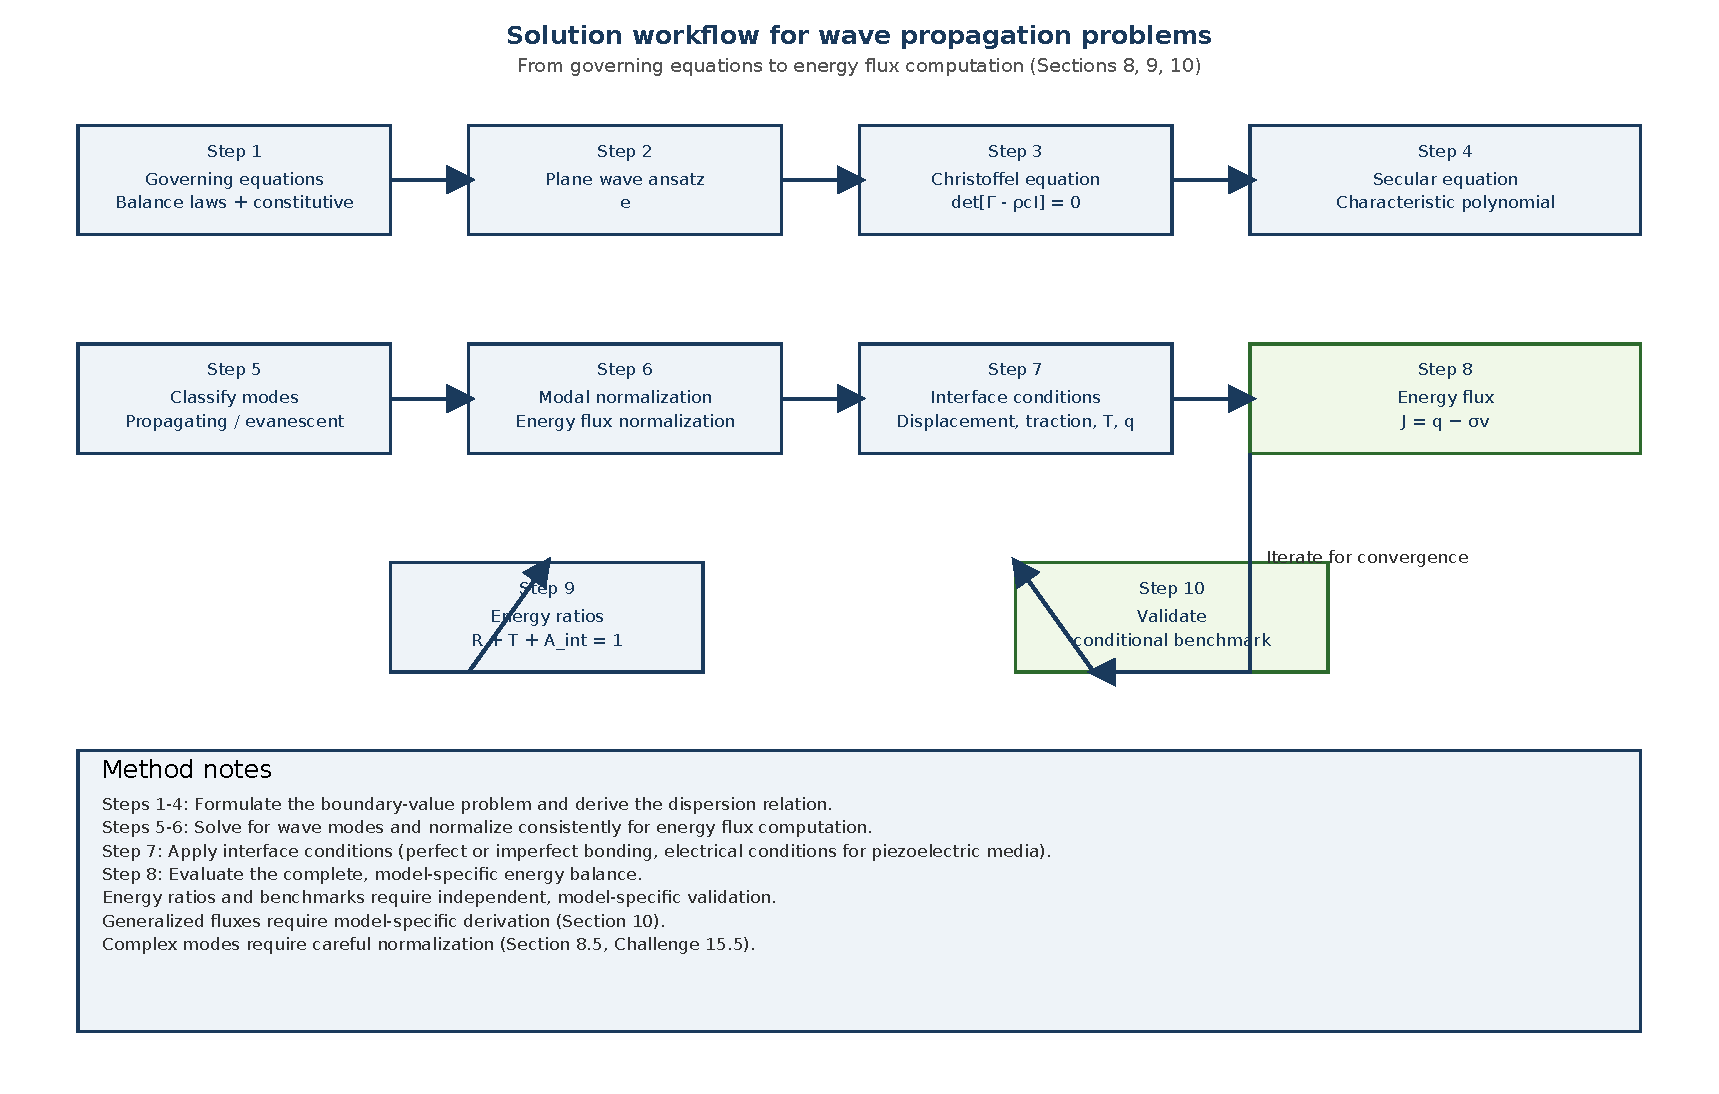
\includegraphics[width=0.95\textwidth]{fig12-solution-workflow.pdf}
\caption{Solution workflow for wave propagation problems: from governing equations to energy flux computation and validation (Sections 8, 9, 10).}
\label{fig:solution_workflow}
\end{figure}

\begin{table}[htbp]
\centering
\small
\setlength{\tabcolsep}{3pt}
\caption{Mathematical techniques used in continuum wave analysis.}
\label{tab:T5-techniques}
\begin{tabularx}{\textwidth}{@{}p{2.4cm}YYYY@{}}
\toprule
\textbf{Technique} & \textbf{Mathematical basis} & \textbf{Typical use} & \textbf{Model-specific consideration} & \textbf{\shortstack{Reference/\\example}} \\
\midrule
Normal mode expansion & Separation of variables; eigenfunction expansion & Layered media and separable geometries & Boundary conditions determine admissible modes & Standard method \\
Green's functions & Fundamental solution and convolution & Point sources and infinite domains & Anisotropy may complicate integral evaluation & Standard method \\
Fourier transform & Frequency-domain representation & Time-harmonic problems and dispersion & Initial-value problems require time-domain treatment & Standard method \\
Laplace transform & Complex-frequency representation & Initial-value problems and transient waves & Inversion may require branch-cut treatment & Standard method \\
Christoffel equation & $\det[\Gamma_{ik}-\rho c^2\delta_{ik}]=0$ & Plane waves in anisotropic media & Polynomial order depends on the field equations & Standard method \\
Scattering matrix & Interface matching formulation & Coupled interface problems & Dimensions and normalization depend on the selected fields & Standard method \\
Finite element & Weak form and variational principles & Complex geometries and nonlinear problems & Mesh choice and computational cost & Standard method \\
\bottomrule
\end{tabularx}
\par\smallskip{\footnotesize These are general method roles; convergence and computational behavior depend on the selected problem, discretization, and implementation.}
\end{table}


\subsection{Notation summary for Section 8}

\begin{table}[htbp]
\centering
\small
\caption{Notation introduced in Section 8.}
\label{tab:notation-sec8}
\begin{tabularx}{\textwidth}{@{}p{1.8cm}X p{2.2cm}p{2.1cm}@{}}
\toprule
\textbf{Symbol} & \textbf{Meaning} & \textbf{Units} & \textbf{Equation} \\
\midrule
$\Gamma_{ik}$ & Christoffel tensor & varies & \eqref{eq:8.2} \\
$c$ & Wave speed & m\,s$^{-1}$ & \eqref{eq:8.2} \\
$q$ & Wave number & m$^{-1}$ & \eqref{eq:8.4} \\
$G_j$ & Coefficients of the secular equation & varies & \eqref{eq:8.4} \\
$\hat{f}(\omega)$ & Fourier transform & varies & \eqref{eq:8.6} \\
$\tilde{f}(s)$ & Laplace transform & varies & \eqref{eq:8.7} \\
$\hat{u}_i^{(n)}$ & Normalized amplitude of mode $n$ & varies & \eqref{eq:8.5} \\
\bottomrule
\end{tabularx}
\end{table}

A layered piezothermoelastic Rayleigh-wave study uses the Green–Naghdi type-III model; its displayed heat equation contains conductivity and additional gradient terms. No energy-partition result is inferred from this example \cite{Biswas2020}.

\subsection{Open questions for Section 8}

\begin{enumerate}[label=\textbf{OQ8.\arabic*}]
\item How are complex modes to be normalized so that the energy ratios computed from them are reproducible across independent implementations, and can a normalization convention be proposed that the field adopts? \label{oq:8.1}
\item How well do numerical schemes converge for nonlocal and memory-dependent models, and what error results from replacing the integral operator by a differential form? \label{oq:8.2}
\item Can the two-stage sequential treatment of the classical problem be extended to the generalized families as an approximation, with a bound on the error introduced? \label{oq:8.3}
\item Which weak formulation is the correct starting point for a variational treatment of a nonlocal and memory-dependent coupled problem? \label{oq:8.4}
\end{enumerate}

% LocalWords:


%======================================================================
% Section 9: Reflection, Transmission, and Interface Phenomena
%======================================================================
%======================================================================
% Section 9: Reflection, Transmission, and Interface Phenomena
%======================================================================
\section{Reflection, Transmission, and Interface Phenomena}
\label{sec:interfaces}

This section presents wave reflection, transmission, and energy partitioning at interfaces between different continuum media. The scattering matrix formulation, interface conditions, and energy ratios are developed for elastic, thermoelastic, and piezothermoelastic media.

\subsection{Interface geometry}
\label{sec:9.1}

Consider two half-spaces in perfect contact at the interface plane $x_3 = 0$. Medium 1 occupies $x_3 < 0$ and medium 2 occupies $x_3 > 0$. A plane harmonic wave is incident from medium 1 onto the interface, generating reflected waves in medium 1 and transmitted waves in medium 2.

The interface normal is $\bm{n} = (0, 0, 1)$. All field variables vary harmonically in time with convention $e^{-i\omega t}$ and propagate along the interface with wave number $k$ in the $x_1$-direction:

\begin{equation}
\text{field}(x_1, x_3, t) = \hat{\text{field}}(x_3) e^{i(kx_1 - \omega t)}.
\label{eq:9.1}
\end{equation}

\subsection{Wave decomposition: incident, reflected, transmitted modes}
\label{sec:9.2}

In each medium, the general solution is a superposition of partial waves. For an isotropic elastic medium, there are two wave types: longitudinal (P) and shear (SV). For thermoelastic media, there is an additional thermal (T) wave. For piezothermoelastic media, there are additional coupled modes (qP, qS, qT, electromagnetic).

The displacement field in medium $m$ ($m = 1, 2$) is decomposed as:

\begin{equation}
u_i^{(m)} = \sum_n A_n^{(m)} \hat{u}_i^{(m,n)} e^{i(q_n^{(m)}x_3 - \omega t)},
\label{eq:9.2}
\end{equation}

where $A_n^{(m)}$ are complex amplitude coefficients, $q_n^{(m)}$ are the vertical wave numbers, and $\hat{u}_i^{(m,n)}$ are the polarization vectors.

The incident wave comes from medium 1 with known amplitude. Reflected waves propagate back into medium 1, and transmitted waves propagate into medium 2.

\subsection{Interface conditions}
\label{sec:9.3}

At a perfectly bonded interface between two media, the following conditions must hold:

\subsubsection{Mechanical conditions}

\begin{equation}
u_i^{(1)} = u_i^{(2)}, \qquad \sigma_{j3}^{(1)} = \sigma_{j3}^{(2)} \quad \text{at } x_3 = 0.
\label{eq:9.3}
\end{equation}

The first condition enforces displacement continuity (no slip or separation); the second enforces traction equilibrium (Newton's third law at the interface).

\subsubsection{Thermal conditions}

For thermoelastic media:

\begin{equation}
T^{(1)} = T^{(2)}, \qquad q_3^{(1)} = q_3^{(2)} \quad \text{at } x_3 = 0.
\label{eq:9.4}
\end{equation}

Temperature continuity and heat flux continuity ensure perfect thermal contact.

\subsubsection{Electrical conditions (piezoelectric media)}

For piezothermoelastic media:

\begin{equation}
\phi^{(1)} = \phi^{(2)}, \qquad D_3^{(1)} = D_3^{(2)} \quad \text{at } x_3 = 0.
\label{eq:9.5}
\end{equation}

Electric potential continuity and electric displacement continuity ensure perfect electrical contact. For an insulated interface, $D_3 = 0$ replaces the second condition.

\subsubsection{Imperfect bonding}

For imperfectly bonded interfaces, spring-type conditions relate displacement jumps to interfacial tractions:

\begin{equation}
u_i^{(2)} - u_i^{(1)} = K_i^u t_i, \qquad \sigma_{j3}^{(1)}n_j = \sigma_{j3}^{(2)}n_j = t_i,
\label{eq:9.6}
\end{equation}

where $K_i^u$ is the interfacial stiffness tensor and $t_i$ is the interfacial traction. In the limit $K_i^u \to \infty$, perfect bonding is recovered; in the limit $K_i^u \to 0$, a traction-free (slip) interface is recovered.

\subsection{Scattering matrix formulation}
\label{sec:9.4}

The interface conditions lead to a linear system relating the unknown amplitude coefficients to the known incident wave amplitude. For a thermo-piezoelastic interface problem with $N$ unknown amplitudes and $N$ interface conditions, the system can be written in matrix form:

\begin{equation}
\Delta \bm{X} = \bm{Q},
\label{eq:9.7}
\end{equation}

where:
\begin{itemize}
\item $\Delta$ is the $N\times N$ system matrix whose entries depend on material properties, wave numbers, frequency, and incidence angle,
\item $\bm{X} = (A_1, A_2, \ldots, A_N)^T$ is the vector of unknown amplitude coefficients (reflected and transmitted),
\item $\bm{Q} = (Q_1, Q_2, \ldots, Q_N)^T$ is the known vector determined by the incident wave amplitude.
\end{itemize}

The entries of $\Delta$ are determined by substituting the partial wave expansions into the interface conditions \eqref{eq:9.3}--\eqref{eq:9.5}. Each row corresponds to one interface condition; each column corresponds to one unknown amplitude.

The solution is obtained by matrix inversion:

\begin{equation}
\bm{X} = \Delta^{-1}\bm{Q}.
\label{eq:9.8}
\end{equation}

The solution exists and is unique when $\det(\Delta) \neq 0$.

\subsection{Secular equation and mode classification}
\label{sec:9.5}

The secular equation (characteristic polynomial) determines the allowed wave numbers in each medium:

\begin{equation}
G_1 q^8 + G_2 q^6 + G_3 q^4 + G_4 q^2 + G_5 = 0,
\label{eq:9.9}
\end{equation}

which is an eighth-order polynomial in $q$ for coupled thermo-piezoelastic media. The roots are classified as:

\begin{itemize}
\item \textbf{Propagating modes:} real $q$ --- waves that propagate without spatial attenuation,
\item \textbf{Evanescent modes:} purely imaginary $q$ --- waves that decay exponentially with distance,
\item \textbf{Attenuating modes:} complex $q$ --- waves that both propagate and attenuate.
\end{itemize}

Only outgoing modes (satisfying the radiation condition) are retained in the physical solution.

\subsection{Number of boundary conditions vs. unknown amplitudes}
\label{sec:9.6}

For a well-posed interface problem, the number of independent boundary conditions must equal the number of unknown amplitude coefficients. Table \ref{tab:T6-interfaces} summarizes interface condition configurations for different interface types.

\begin{figure}[htbp]
\centering
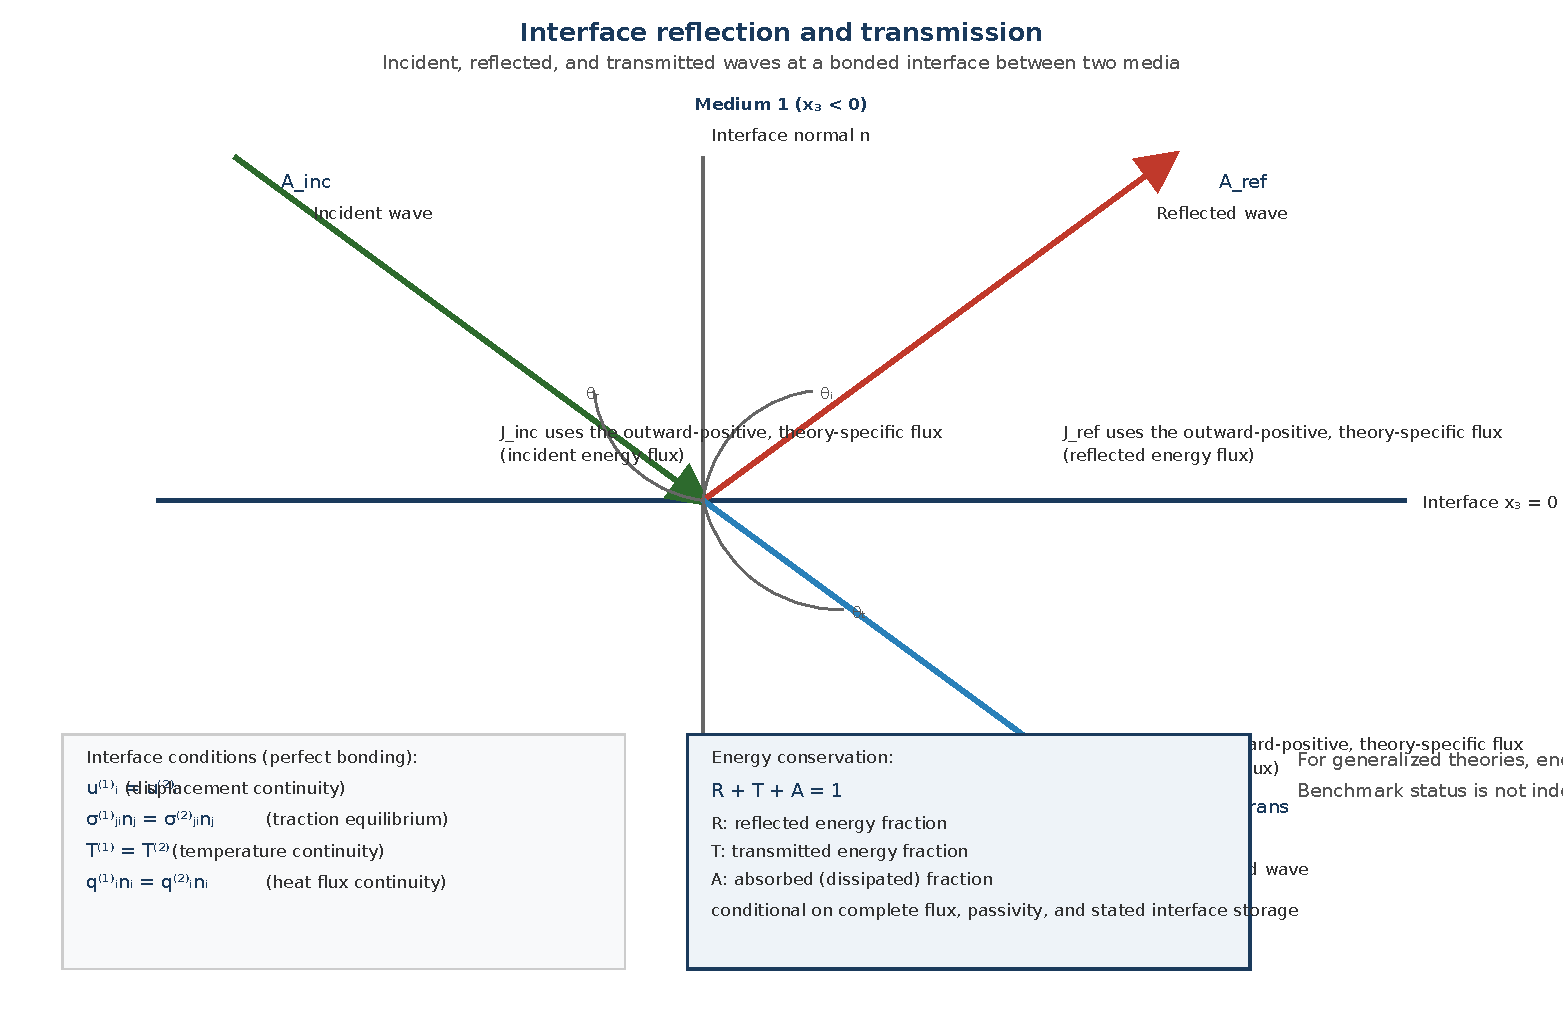
\includegraphics[width=0.9\textwidth]{fig13-interface-reflection.pdf}
\caption{Interface reflection and transmission geometry: incident P-wave from Medium 1 generates reflected P and S waves in Medium 1 and transmitted qP and qS waves in Medium 2. Interface conditions enforce displacement, traction, temperature, heat flux, electric potential, and electric displacement continuity.}
\label{fig:interface_geometry}
\end{figure}

%======================================================================
% Table T6 — Reflection and transmission configurations
% Section: §9
% Inherited interface summary; conditions and evidence require model-specific checks
%======================================================================
\begin{table}[htbp]
\centering
\small
\setlength{\tabcolsep}{3pt}
\caption{Reflection and transmission interface configurations. Matching conditions and modal phenomena for bonded and imperfect interfaces.}
\label{tab:T6-interfaces}
\begin{tabularx}{\textwidth}{@{}p{2.4cm}YYYY@{}}
\toprule
\textbf{Configuration} & \textbf{Matching Conditions} & \textbf{Modal Phenomena} & \textbf{Physical Quantities} & \textbf{Evidence} \\
\midrule
Welded interface (perfect bonding) & $u_i^{(1)}=u_i^{(2)}$; $\sigma_{ji}^{(1)}n_j=\sigma_{ji}^{(2)}n_j$ & Mode conversion; P--S conversion; interface waves & $R,T,A_{\mathrm{int}}$; total-field identity; $A_{\mathrm{int}}=0$ if passive, lossless, and no interfacial storage & Standard theory \\
Imperfect (spring-type) interface & Displacement jump proportional to traction & Partial transmission; interface stiffness effects & Transmission coefficient dependent on spring stiffness & Model-specific \\
Perfect thermal contact & $T^{(1)}=T^{(2)}$; $q_i^{(1)}n_i=q_i^{(2)}n_i$ & Thermal-field transmission/reflection; propagating modes only in finite-speed models & Continuous temperature and normal heat flux & Perfect-contact idealization \\
Kapitza (imperfect thermal contact) & $q_n^{(1)}=q_n^{(2)}$; $T^{(2)}-T^{(1)}=R_K q_n$ & Temperature jump at finite heat flux & Interfacial thermal resistance $R_K$ & Model-specific; sign follows chosen normal \\
Electrical interface & $\phi^{(1)}=\phi^{(2)}$; $D_i^{(1)}n_i=D_i^{(2)}n_i$ & Piezoelectric coupling; surface charge & Electric displacement continuity if free surface charge is zero; otherwise its jump is the surface charge density & Standard theory \\
Thermo-piezoelastic interface & All mechanical, thermal, electrical conditions & Multi-field scattering; energy partitioning & Interface-energy study cited; equation-level claims not checked & \cite{Barak2023} \\
\bottomrule
\multicolumn{5}{@{}p{\textwidth}@{}}{\textbf{Notes:} The proposed BM-1 conservation check was not executed in this revision; see Appendix C.}\\
\multicolumn{5}{@{}p{\textwidth}@{}}{\emph{Thermo-piezoelastic interface equations and cited energy ratios are inherited claims, not checked against the full source here.}}\\
\end{tabularx}
\end{table}


\subsection{Energy ratios at interfaces}
\label{sec:9.7}

The energy reflection coefficient $R$, transmission coefficient $T$, and absorption coefficient $A$ are defined as:

\begin{equation}
R = \frac{|\avg{J_{\mathrm{ref},n}}_t|}{|\avg{J_{\mathrm{inc},n}}_t|},
\qquad
T = \frac{|\avg{J_{\mathrm{trans},n}}_t|}{|\avg{J_{\mathrm{inc},n}}_t|},
\qquad
A = \frac{\mathcal{D}}{|\avg{J_{\mathrm{inc},n}}_t|},
\label{eq:9.10}
\end{equation}

where the averages are time averages over one period and $n$ is the interface normal.

For a conservative system with no dissipation ($\mathcal{D} = 0$) and a passive interface:

\begin{equation}
\sum R + \sum T = 1.
\label{eq:9.11}
\end{equation}

With dissipation:

\begin{equation}
\sum R + \sum T + A = 1.
\label{eq:9.12}
\end{equation}

The identity \eqref{eq:9.12} holds when the energy flux is correctly defined for the specific theory, the interface is passive, all modes are properly accounted for, and complex modes are consistently normalized.

This makes interface energy analysis unusually stringent as a test of a generalized theory: the same identity must close for every model in the family, and any inconsistency between the flux used in the numerators and the dissipation used in the denominator shows up immediately as a violation. The recent literature has exploited that sensitivity to quantify how relaxation, memory and anisotropy redistribute energy across a bonded boundary, and the results fall into a small number of recurring patterns.

\subsubsection{What the interface partition reveals}

The energy partition at an interface is a far more sensitive probe of a constitutive model than any bulk measurement, for a reason that is structural rather than accidental: the interface condition set is the only place in the problem where all the couplings are exercised simultaneously and where a single scalar identity must close. The identity of \eqref{eq:9.12} does not distinguish between two theories that agree in the bulk but differ in how they transmit energy; the reflected and transmitted fractions do.

Four distinct mechanisms of energy redistribution have been quantified on this basis, and it is worth separating them, because they are frequently conflated.

\begin{enumerate}
\item \textbf{Electromechanical renormalisation.} At a boundary between an elastic and a piezothermoelastic half-space, the transmitted energy budget is altered not by a new dissipation mechanism but by the renormalisation of the elastic stiffness that the electromechanical coupling induces. The conservation identity remains satisfied, and the shift in the transmitted fraction is a stiffness effect rather than an absorption effect \cite{Barak2023IJP}. This is the cleanest demonstration in the reviewed literature that a generalized theory can change an observable while leaving the thermodynamics untouched.
\item \textbf{Extra attenuation channels.} When the thermoelastic partner is replaced by a medium with additional internal degrees of freedom --- a dual-porous solid, with its permeability-dependent relaxation and its phase-lag structure --- additional attenuation channels open, and the energy-ratio curves vary with incidence angle in a manner that no single-phase treatment reproduces \cite{Kumar2023PhysScr}. The diagnostic content lies in the angular dependence, not merely in the value at normal incidence.
\item \textbf{History-dependent transmission.} Memory-dependent heat conduction changes the transmitted thermal energy through the kernel-weighted history of the flux, and the change depends jointly on the delay parameter of the kernel and on the stiffness contrast across the interface \cite{Barak2023MMMS}. The same dependence persists when monoclinic anisotropy is added to the piezothermoelastic partner \cite{Barak2023JTS}, which indicates that the two generalizations act through separate mechanisms and can therefore be separated experimentally by varying the interface contrast at fixed anisotropy.
\item \textbf{Nonlocal phase shifts at a fluid boundary.} At a fluid/solid boundary, where the first medium carries no elastic field and the transmitted set is constrained by the kinematic admissibility conditions of the fluid, a nonlocal length scale in the solid modifies the phase of the reflected and transmitted waves while leaving the energy balance closed \cite{Gupta2023IJNMF}. Here the nonlocality shows itself in phase rather than in energy, which is the clearest available signature that distinguishes it from a purely dissipative effect.
\end{enumerate}

Two further results complete the picture. For a piezoelectric/thermoelastic interface the full energy analysis across the coupled fields shows that the electrical contribution does not decouple from the mechanical one, so that a single-field energy budget is not adequate and a coupled flux must be constructed \cite{Gupta2023Energy}. And a compact scattering-matrix treatment of this interface class, in which the amplitude system is written as a single matrix relation rather than as a set of separate modal equations, together with its higher-order memory-dependent variant, has been given for the same configuration \cite{Barak2023}.

\subsubsection{The pattern and its limits}

Across this body of work the pattern is consistent: the conservation identity survives extension to generalized media, but only when the energy flux is reconstructed from the constitutive model actually being solved. The difficulty identified in Section~\ref{sec:energy} is therefore not that the identity fails, but that a general-purpose expression for that flux has not been written down for every member of the family. A second limit is worth recording. All of the configurations above assume a perfectly bonded, flat interface between two homogeneous half-spaces with sharp material contrast. Real interfaces are graded over a thickness comparable with the microstructural length, and for nonlocal, memory-dependent and gradient theories the thickness of the interfacial layer is not negligible compared with the internal length of the material. Whether the sharp-interface result is the limit of a graded-interface result, and at what rate, is an open question that no configuration in the reviewed literature addresses.

\subsection{Interface conditions under memory and nonlocality}
\label{sec:9.8}

The interface conditions of Section~\ref{sec:9.3} assume that the constitutive variables are local functions of position. This assumption fails in two of the theory families treated here, and the failure has a common structure: the quantity that is matched across the interface is no longer a pointwise value.

For a \emph{memory-dependent} medium, the flux at the interface is an integral over the recent past, and a naive condition of the form $q_3^{(1)} = q_3^{(2)}$ matches two functionals whose histories differ. The condition is either imposed on the effective flux of \eqref{eq:6.10} --- in which case the identity of Section~\ref{sec:energy} must already have been established --- or imposed on the constitutive variables together with their history, in which case the interface problem becomes an initial-value problem in the tangential coordinate and its solution depends on how the interface was approached.

For a \emph{nonlocal} medium, the stress at the interface is an average over a neighbourhood that straddles the interface, so that the traction transmitted across the interface is not a pointwise quantity at all; the correct interface problem is then a nonlocal boundary-value problem in which the interface condition couples the two half-spaces over the whole interfacial region. A local approximation that simply writes $t_i^{(1)} = t_i^{(2)}$ is consistent only to leading order in the ratio of the internal length to the wavelength.

Neither of these is merely a technical difficulty. Both concern the meaning of an interface in a theory that has no microscopic notion of a material boundary, and both are of the same character as the question of whether the constitutive variables of a nonlocal or memory-dependent theory can be continued across a material discontinuity at all. These are recorded as open questions in Section~\ref{sec:future}; they are the places where the extension of the classical framework to generalized media is least settled.

\subsection{Notation summary for Section 9}

\begin{table}[htbp]
\centering
\small
\caption{Notation introduced in Section 9.}
\label{tab:notation-sec9}
\begin{tabularx}{\textwidth}{@{}lXlr@{}}
\toprule
\textbf{Symbol} & \textbf{Meaning} & \textbf{Units} & \textbf{Equation} \\
\midrule
$A_n^{(m)}$ & Complex amplitude coefficient & varies & \eqref{eq:9.2} \\
$q_n^{(m)}$ & Vertical wave number & 1/m & \eqref{eq:9.2} \\
$\Delta$ & System matrix & varies & \eqref{eq:9.7} \\
$\bm{X}$ & Unknown amplitude vector & varies & \eqref{eq:9.7} \\
$\bm{Q}$ & Known incident vector & varies & \eqref{eq:9.7} \\
$R, T, A$ & Reflection, transmission, absorption coefficients & dimensionless & \eqref{eq:9.10} \\
$K_i^u$ & Interfacial stiffness & varies & \eqref{eq:9.6} \\
\bottomrule
\end{tabularx}
\end{table}

\subsection{Open questions for Section 9}

\begin{enumerate}[label=\textbf{OQ9.\arabic*}]
\item What are the interface conditions for nonlocal media where stress depends on strain in a neighborhood? \\ \label{oq:9.1}
\item How are energy ratios computed for memory-dependent media with hereditary flux? \\ \label{oq:9.2}
\item What is the correct interface energy balance for piezothermoelastic media with electrical coupling? \\ \label{oq:9.3}
\item Is the sharp-interface result the limit of a graded-interface result for nonlocal, gradient and memory-dependent media, and at what rate does the difference vanish as the interfacial layer is thickened? \\ \label{oq:9.4}
\item Can the constitutive variables of a nonlocal or memory-dependent theory be continued across a material discontinuity at all, and what does that imply for the meaning of an interface in such a theory? \\ \label{oq:9.5}
\end{enumerate}

% LocalWords:


%======================================================================
% Section 10: Energy Transport and Dissipation
%======================================================================
%======================================================================
% Section 10: Energy Transport and Dissipation
%======================================================================
\section{Energy Transport and Dissipation}
\label{sec:energy}

Constitutive theories carry energy-storage, transport, and dissipation consequences, but the expressions depend on their state variables and field equations. This section derives the classical local flux under explicit conventions, states the interface balance at a general level, and records family-specific flux claims as open unless their free energy, constitutive evolution, boundary power, and dissipation inequality have been checked. No universal generalized-continuum flux is assumed.

\subsection{General energy balance}
\label{sec:10.1}

For classical thermoelasticity, with specific internal energy $e$, the total energy per unit volume is

\begin{equation}
\mathcal{E} = \frac{1}{2}\rho v_i v_i + \rho e,
\label{eq:10.1}
\end{equation}

and, with no internal heat source, the exact Eulerian balance is

\begin{equation}
\frac{\partial\mathcal{E}}{\partial t} + \partial_i F_i = \rho f_i v_i,
\qquad F_i=q_i-\sigma_{ij}v_j+\mathcal{E}v_i,
\label{eq:10.2}
\end{equation}

where $\rho f_i v_i$ is mechanical power per unit volume and $F_i$ is the exact Eulerian flux for the classical local Cauchy continuum. Equation~\eqref{eq:10.2} is not asserted as a universal generalized-multiphysics identity: additional field energy, external electrical or magnetic power, interface storage, and internal dissipation must be derived for each specified model.

\subsection{Classical energy flux}
\label{sec:10.2}

For first-order small-amplitude fields about a resting reference state, after measuring $e$ relative to a constant $e_0$, the perturbation advection $\rho[\tfrac12 v_jv_j+(e-e_0)]v_i$ is $O(\epsilon^2)$ and is absent from the first-order field balance. The reduced outward-positive flux used below is

\begin{equation}
J_i = q_i - \sigma_{ij}v_j,
\label{eq:10.3}
\end{equation}
It is not the exact Eulerian total-energy flux: the latter is $F_i=J_i+\mathcal{E}v_i$ as in Eq.~\eqref{eq:10.2}. The reduced expression is used only for the stated first-order wave-balance convention; this order argument alone does not justify omitting the advective term from a second-order cycle-averaged total-energy flux. Under the outward-positive convention the mechanical contribution is $-\sigma_{ij}v_j$ and the thermal contribution is $q_i$.

For time-harmonic mechanical fields with convention $e^{-i\omega t}$, the mean of the reduced flux is

\begin{equation}
\langle J_i\rangle_t=\bar q_i-\frac12\Re[\hat{\sigma}_{ij}\hat{v}_j^*],
\label{eq:10.4}
\end{equation}

where $\bar q_i$ is the separately evaluated mean heat flux (zero for a purely oscillatory perturbation about a uniform reference state). The factor $1/2$ and complex conjugate follow from time averaging the real fields. For an interface problem using this reduced convention the quantity is $J_n=J_i n_i$. If a second-order Eulerian total-energy balance is claimed, the mean of the advective contribution must also be evaluated or shown to vanish under an additional model-specific assumption.

A point worth keeping in view is that the reduced classical flux contains \emph{no} term associated with the internal variables that generalized theories introduce. The entire difficulty of Section~\ref{sec:10.4} follows from that absence.





\subsection{Interface energy balance}
\label{sec:10.3}

Consider a stationary interface $\Sigma$ between two media with unit normal $\bm{n}$. Integrating the model-correct total-energy balance over a thin pillbox straddling the interface and taking the thinness limit gives the jump condition

\begin{equation}
\jump{\mathcal{F}_n} = \mathcal{P}_\Sigma - \frac{\partial\mathcal{E}_\Sigma}{\partial t},
\label{eq:10.5}
\end{equation}
where $\mathcal{F}_n=\mathcal{F}_i n_i$ is the normal component of the exact, model-correct Eulerian total-energy flux (equal to $F_n$ for the classical continuum), $\mathcal{P}_\Sigma$ is the mechanical power input at the interface, and $\mathcal{E}_\Sigma$ is the interfacial energy density. The reduced $J_i$ of Eq.~\eqref{eq:10.3} may replace it only within the stated first-order approximation.

For a passive interface with no mechanical power input and no interfacial energy storage,

\begin{equation}
\jump{\mathcal{F}_n} = 0,
\label{eq:10.6}
\end{equation}
that is, the normal model-correct total-energy flux is continuous across the interface. Two qualifications are needed before this condition is used numerically. First, it is a statement about the \emph{correct} energy flux of the theory in which it is used; a flux built from the classical form alone, applied to a family with internal variables, will not satisfy it even when the mathematics is otherwise flawless. Second, the continuity of the normal flux does not by itself imply the scalar conservation identity of Section~\ref{sec:10.5}: that identity is a statement about modal energies, while \eqref{eq:10.6} is a statement about a single component of a flux at a single surface, and the two are related only after the modal decomposition and normalisation conventions have been fixed.

\subsection{Energy transport in generalized theories: the internal-variable structure}
\label{sec:10.4}

The first-law balance retains the boundary power terms for a specified constitutive theory. What changes between generalized theories is the stored free energy and dissipation, which follow from that theory's state variables and evolution laws. There is no universal additional flux term $-\sum_\alpha Y^\alpha\dot z^\alpha$: this has units of power per volume, not energy flux, unless an additional spatial transport structure is specified. A family-specific identity therefore requires the model's free energy, evolution law, and boundary terms.

\subsubsection{Piezothermoelastic energy flux}

For a coupled piezothermoelastic model, the mechanical, electrical, and thermal power terms should be derived from one stated balance convention and the coupled constitutive equations before modal ratios are interpreted.

\subsubsection{Energy flux in generalized theories}

A family-specific energy balance requires the free energy, flux variables, boundary powers, dissipation terms, and constitutive equations of the selected model.

For the surface thermoelastic waves studied by Ivanov and Savova, the energy-flux vector connected with kinetic and internal energy is reported as not parallel to the half-space surface; its direction varies with distance from the surface, its magnitude decays to zero with depth, and it decays exponentially along the direction in which the superposed waves' constant-phase planes intersect the surface (printed p.~564). This is a paper-specific surface-wave result, not a universal flux law \cite{IvanovSavova1991}.

\subsection{Remote-plane energy partition}
\label{sec:10.5}

For passive regions with steady time-averaged powers, no source, no net energy accumulation, and no unlisted energy channel, the remote-plane balance is

\begin{equation}
R_{\mathrm{rem}} + T_{\mathrm{rem}} + A_{\mathrm{bulk},L} + A_{\mathrm{int}} + A_{\mathrm{bulk},R} = 1,
\label{eq:10.11}
\end{equation}

where $R_{\mathrm{rem}}=P_r/P_i$ and $T_{\mathrm{rem}}=P_t/P_i$ use positive incident/reflected/transmitted power magnitudes at explicitly stated remote reference planes. The normalized losses are $A_{\mathrm{bulk},L}=\mathcal{D}_L/P_i$, $A_{\mathrm{int}}=\mathcal{D}_{\Sigma}/P_i$, and $A_{\mathrm{bulk},R}=\mathcal{D}_R/P_i$, with the control-volume powers defined in Eq.~\eqref{eq:10.13}. This is distinct from the interface-plane bookkeeping identity in Section~\ref{sec:9.7}; when bulk attenuation separates the planes, $1-R_{\mathrm{rem}}-T_{\mathrm{rem}}$ includes both bulk losses and the local interface residual. Only when the bulk losses and interface residual vanish does the remote-plane balance reduce to

\begin{equation}
R_{\mathrm{rem}} + T_{\mathrm{rem}} = 1.
\label{eq:10.12}
\end{equation}

Kumar and Kansal report a model-specific interface energy-ratio balance with an interaction term in Eq. (80), supporting inclusion of cross terms rather than a universal identity \cite{KumarKansal2017}. Kumar et al. define ratios using average energy flux per incident-wave type; those definitions specify normalization but do not establish closure \cite{Kumar2024}. A related study describes its eight-model sum as approximately unity for specified imperfect-interface cases; this is model-specific evidence, not an identity \cite{Kumar2024a}.

Equation~\eqref{eq:10.11} is the steady control-volume balance under the stated assumptions; its application requires the theory-specific flux, complete power channels, interface storage/power convention, and common remote reference planes. It is not the interface-plane identity of Section~\ref{sec:9.7}. The lossless reduction additionally requires zero bulk loss, zero interface-local residual, and no net interfacial storage. These conditions are not automatic. In the one-dimensional welded example below, the incident--reflected cross term cancels in the time-averaged normal flux; no zero-flux rule for general coupled or evanescent modes is inferred. Report whether each coefficient is an amplitude or a power ratio and state the flux weighting used.

\subsubsection{Separate interface residual from bulk absorption}

Consider a steady time-averaged one-dimensional control volume and take $+x$ as the positive normal direction. Let $\mathcal{F}_x^{(i)}$, $\mathcal{F}_x^{(r)}$, and $\mathcal{F}_x^{(t)}$ denote the incident-, reflected-, and transmitted-mode contributions to the model-correct Eulerian energy flux at stated remote reference planes, with the exact flux used unless a reduced convention is explicitly justified. Per unit cross-sectional area $A$, define $P_i=A^{-1}\int_{S_i}\langle\mathcal{F}^{(i)}\rangle\cdot\hat{\bm{x}}\,dS>0$, $P_r=-A^{-1}\int_{S_r}\langle\mathcal{F}^{(r)}\rangle\cdot\hat{\bm{x}}\,dS>0$, and $P_t=A^{-1}\int_{S_t}\langle\mathcal{F}^{(t)}\rangle\cdot\hat{\bm{x}}\,dS>0$. The selected remote-plane decomposition must make the net left-plane flux equal to $P_i-P_r$; if an incident--reflected cross term remains there, it must be included explicitly in the power balance. Let $\mathcal{F}_L$ and $\mathcal{F}_R$ be the net total-field fluxes on the left and right faces of the interface, both oriented in $+x$. For passive, source-free regions with no bulk or interfacial mean energy accumulation, the bulk and interfacial dissipated powers per unit area are

\begin{equation}
\mathcal{D}_L=P_i-P_r-\mathcal{F}_L,\qquad
\mathcal{D}_{\Sigma}=\mathcal{F}_L-\mathcal{F}_R,\qquad
\mathcal{D}_R=\mathcal{F}_R-P_t.
\label{eq:10.13}
\end{equation}

Summing the three control-volume balances gives

\begin{equation}
P_i=P_r+P_t+\mathcal{D}_L+\mathcal{D}_{\Sigma}+\mathcal{D}_R.
\label{eq:10.14}
\end{equation}

Thus, with $R_{\mathrm{rem}}=P_r/P_i$ and $T_{\mathrm{rem}}=P_t/P_i$, the remote-plane residual $1-R_{\mathrm{rem}}-T_{\mathrm{rem}}$ already contains both bulk dissipation and local interface dissipation. By contrast, $A_{\mathrm{int}}=\mathcal{D}_{\Sigma}/P_i=(\mathcal{F}_L-\mathcal{F}_R)/P_i$ is local to the interface. Adding the bulk terms to $1-R_{\mathrm{rem}}-T_{\mathrm{rem}}$ a second time double-counts them; this follows directly by summing Eqs.~\eqref{eq:10.13}--\eqref{eq:10.14}. The derivation assumes steady averaged powers, no storage in the bulk control volumes, and no unlisted energy channel; other theories require their complete energy flux and power terms.

\subsubsection{Worked one-dimensional welded-interface system}

For a normal-incidence longitudinal wave at $x=0$ in two lossless one-dimensional bars, let $c_m$ be each bar's longitudinal wave speed and take real positive impedances $Z_m=\rho_m c_m$ and wave numbers $k_m=\omega/c_m$. Under the $e^{-i\omega t}$ convention, the displacement amplitudes are

\begin{equation}
\hat u_1=A_i e^{ik_1x}+A_r e^{-ik_1x},\qquad
\hat u_2=A_t e^{ik_2x}.
\label{eq:10.15}
\end{equation}

Displacement and traction continuity, using $\hat\sigma_{xx}=\rho_m c_m^2\partial_x\hat u_m$, give $A_i+A_r=A_t$ and $Z_1(A_i-A_r)=Z_2A_t$. With $A_r$ and $A_t$ as the two unknown amplitudes, these are two scalar conditions and yield the $2\times2$ system

\begin{equation}
\begin{bmatrix}1&-1\\-Z_1&-Z_2\end{bmatrix}
\begin{bmatrix}A_r\\A_t\end{bmatrix}
=-A_i\begin{bmatrix}1\\Z_1\end{bmatrix}.
\label{eq:10.16}
\end{equation}

Its determinant is $-(Z_1+Z_2)$, so the stated positive-impedance case has a unique solution, with amplitude ratios $r=A_r/A_i=(Z_1-Z_2)/(Z_1+Z_2)$ and $t=A_t/A_i=2Z_1/(Z_1+Z_2)$. For the mechanical flux $\langle J_x\rangle=-\tfrac12\Re[\hat\sigma_{xx}\hat v_x^*]$, the incident and reflected power ratios are $R=|r|^2$ and $T=(Z_2/Z_1)|t|^2$. These coincide with the remote-plane ratios because this welded example has lossless, non-attenuating half-spaces. Direct substitution gives $R+T=1$; this result is not asserted for an imperfect, dissipative, or generalized interface. To show the incident/reflected cross term rather than assume it away, the same-medium fields in Eq.~\eqref{eq:10.15} give $\hat v_i=-i\omega A_i e^{ik_1x}$, $\hat\sigma_i=ik_1\rho_1c_1^2 A_i e^{ik_1x}$, $\hat v_r=-i\omega A_r e^{-ik_1x}$, and $\hat\sigma_r=-ik_1\rho_1c_1^2 A_r e^{-ik_1x}$. Before taking the real part in the harmonic flux, their mixed product is
\begin{equation*}
\hat\sigma_i\hat v_r^*+\hat\sigma_r\hat v_i^*=\rho_1c_1^2 k_1\omega\left[-A_iA_r^*e^{2ik_1x}+A_rA_i^*e^{-2ik_1x}\right],
\end{equation*}
the negative of a complex number plus its conjugate, and therefore purely imaginary; hence its time-averaged normal-flux contribution $-\tfrac12\Re(\hat\sigma_i\hat v_r^*+\hat\sigma_r\hat v_i^*)$ is zero. This cancellation is derived only for the stated one-dimensional, lossless longitudinal waves. Direct substitution verifies the matrix dimensions, determinant, amplitudes, field-derived flux weights, cross term, and partition identity for this specified one-dimensional case.

\subsection{Dissipation mechanisms}
\label{sec:10.6}

Dissipative mechanisms can include heat-flux relaxation, viscous stress, dielectric loss, interfacial friction, or hereditary memory. Their presence and non-negative dissipation conditions depend on the precise constitutive equations and admissible state space. A single scalar dissipation function or common parameter-ordering rule does not apply uniformly across these families. In particular, the condition $\tau_q\geq\tau_T\geq0$ and a positive Lord--Shulman relaxation time are not, by themselves, a full proof of thermodynamic admissibility or stability. Deriving model-specific free energies and dissipation inequalities remains open.

\subsection{Thermodynamic admissibility: well-posedness, causality, positivity}
\label{sec:10.7}

Thermodynamic admissibility, mathematical well-posedness, and finite-speed propagation are distinct questions. A constitutive theory requires its own free-energy/entropy statement and dissipation inequality; an initial-boundary-value problem requires a separate existence, uniqueness, and continuous-dependence analysis; propagation speed is a property of the selected equations and parameter regime. Fourier heat conduction gives a parabolic equation with instantaneous mathematical support. Statements for relaxation, phase-lag, memory, fractional, and gradient models depend on their exact constitutive laws.

\subsection{Comparative table: energy transport across theory families}

Table~\ref{tab:energy_transport} summarizes the classical flux and model-specific terms relevant to generalized energy balances.



\begin{table}[htbp]
\centering
\caption{Energy-flux structures by constitutive family.}
\label{tab:energy_transport}
\begin{tabularx}{\textwidth}{@{}p{2.5cm}XX@{}}
\toprule
\textbf{Theory family} & \textbf{Energy/flux structure} & \textbf{Terms specific to the selected model} \\
\midrule
Classical thermoelasticity & $\mathcal{E}=\tfrac12\rho v_i v_i+\rho e$; exact Eulerian $F_i=q_i-\sigma_{ij}v_j+\mathcal{E}v_i$; reduced first-order $J_i=q_i-\sigma_{ij}v_j$ & Heat-flux constitutive law and boundary power \\
Generalized constitutive families & Model-specific stored energy and flux & Evolution equations, internal variables, boundary power, and dissipation terms \\
\bottomrule
\multicolumn{3}{@{}p{\textwidth}@{}}{\footnotesize No universal flux formula is implied for the generalized families.}\\
\end{tabularx}
\end{table}


\begin{figure}[htbp]
\centering
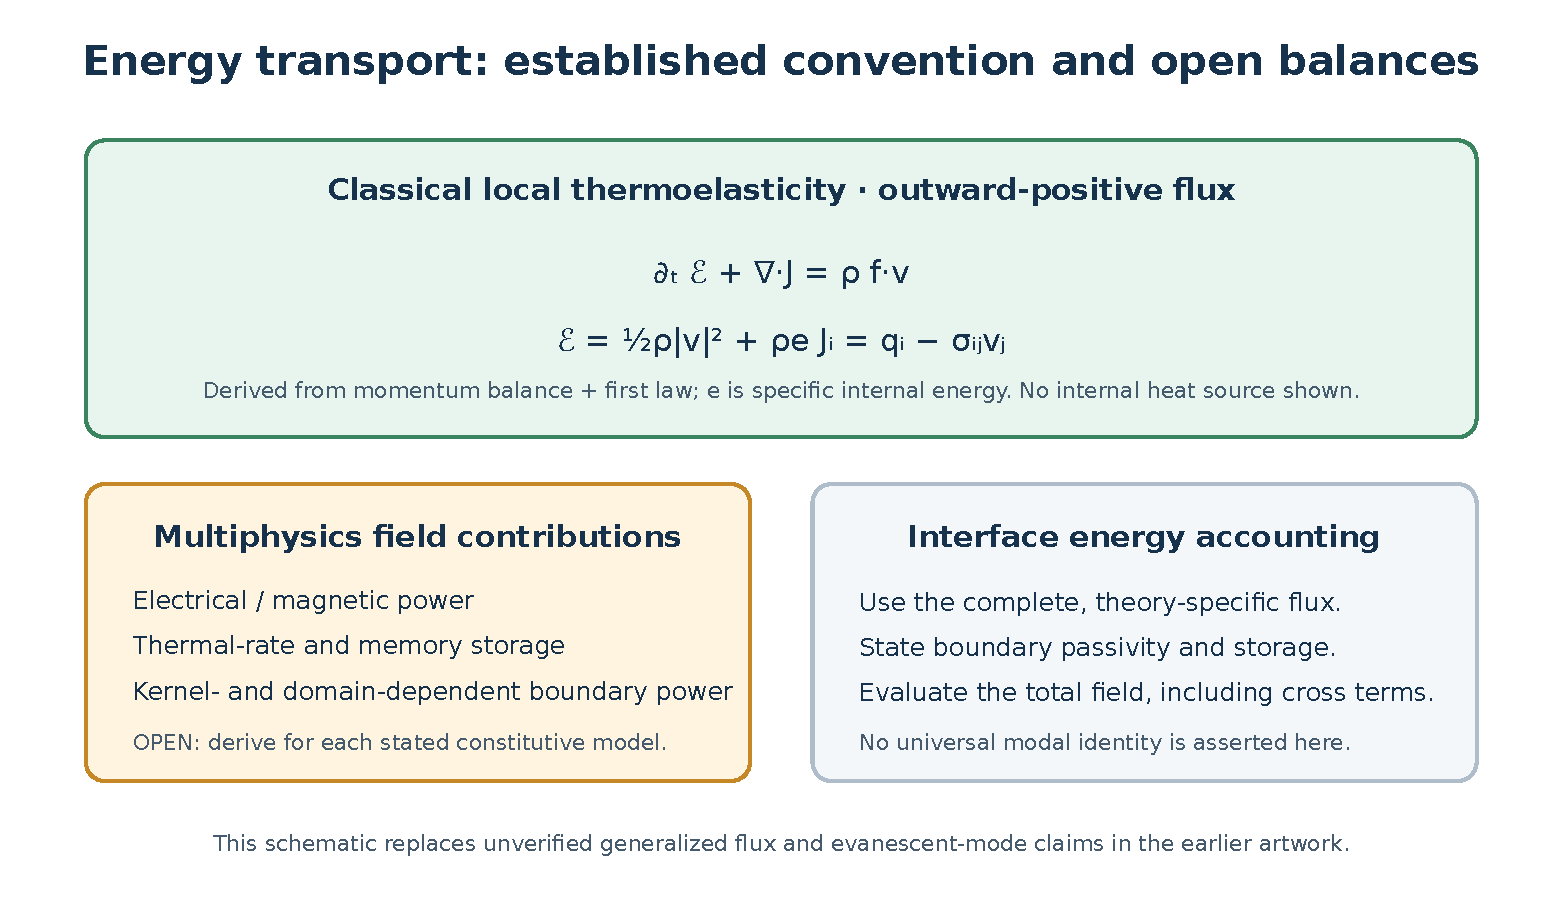
\includegraphics[width=0.9\textwidth]{fig14-energy-flux-channels.pdf}
\caption{Energy-balance conventions and open flux audit. The classical local thermoelastic flux is derived under the stated outward-positive convention; generalized multiphysics contributions and modal energy identities remain open pending model-specific derivations.}
\label{fig:energy_flux}
\end{figure}

\subsection{Notation summary for Section 10}

\begin{table}[htbp]
\centering
\small
\caption{Notation introduced in Section 10.}
\label{tab:notation-sec10}
\begin{tabularx}{\textwidth}{@{}p{1.8cm}X p{2.2cm}p{2.1cm}@{}}
\toprule
\textbf{Symbol} & \textbf{Meaning} & \textbf{Units} & \textbf{Equation} \\
\midrule
$\mathcal{E}$ & Total energy density & J\,m$^{-3}$ & \eqref{eq:10.1} \\
$\bm{J}$ & Energy flux vector & W\,m$^{-2}$ & \eqref{eq:10.2} \\
$\mathcal{P}$ & Mechanical power input & W\,m$^{-3}$ & \eqref{eq:10.2} \\
$J_i$ & Classical energy flux component & W\,m$^{-2}$ & \eqref{eq:10.3} \\
$\avg{J_i}_t$ & Time-averaged energy flux & W\,m$^{-2}$ & \eqref{eq:10.4} \\
$\mathcal{E}_\Sigma$ & Interfacial energy density & J\,m$^{-2}$ & \eqref{eq:10.5} \\
$\mathcal{P}_\Sigma$ & Interfacial power input & W\,m$^{-2}$ & \eqref{eq:10.5} \\
$R, T, A$ & Reflection, transmission, absorption coefficients & dimensionless & \eqref{eq:10.11} \\
\bottomrule
\end{tabularx}
\end{table}

\subsection{Open questions for Section 10}

\begin{enumerate}[label=\textbf{OQ10.\arabic*}]
\item What is the explicit time-domain energy flux and dissipation function for each of the families listed in Section~\ref{sec:10.4}, derived from that family's free energy, evolution laws, and boundary-power terms? \label{oq:10.1}
\item Is there a common formal structure under which the energy fluxes of the Lord--Shulman, phase-lag, Moore--Gibson--Thompson, and memory-dependent families become instances of a single template, so that a single derivation suffices for all of them? \label{oq:10.2}
\item Which observable would distinguish the energy partition predicted by two competing theories at the same interface, so that the difference could be measured rather than argued? \label{oq:10.3}
\item How should the entropy production of the conservative Green--Naghdi type~II structure be related to the entropy production of the dissipative branches, given that the former has no dissipation mechanism? \label{oq:10.4}
\item What normalisation of complex modes makes the energy ratios of Eq.~\eqref{eq:10.11} reproducible across independent implementations? \label{oq:10.5}
\item Can a dissipation potential be constructed for the memory-dependent kernel in the spirit of the classical one for the relaxation terms, and does its positivity restrict the admissible kernels to a smaller set than is currently assumed? \label{oq:10.6}
\item What is the relative importance of interface dissipation and bulk dissipation in the absorption coefficient of Eq.~\eqref{eq:10.11} for realistic bonded joints? \label{oq:10.7}
\end{enumerate}

% LocalWords:


%======================================================================
% Section 11: Advanced Theoretical Developments
%======================================================================
%======================================================================
% Section 11: Advanced Theoretical Developments
%======================================================================
\section{Advanced Theoretical Developments}
\label{sec:advanced}

The theory families of Sections~\ref{sec:thermoelastic}--\ref{sec:nonlocal} were each constructed by generalising one specific constitutive law. The developments surveyed in this section generalise the generalisation: they act on the \emph{operator} rather than on the constitutive law, and they therefore interact with every family simultaneously. Two of them---fractional-order differentiation and the introduction of additional temperature fields---are now established enough to be treated as substantive alternatives rather than as speculative extensions, and this section gives them the same weight as the classical constructions of Section~\ref{sec:thermoelastic}.

\subsection{Fractional-order continuum models}
\label{sec:11.1}

Fractional-order continuum models replace integer-order derivatives with fractional derivatives in the governing equations. The replacement is not a formal device: a fractional derivative of order $\alpha$ is defined by an integral over the entire history of the field, and it therefore introduces temporal nonlocality into the governing equations in a way that is structurally equivalent to a hereditary integral with a power-law kernel.

\subsubsection{Fractional thermoelasticity}

The fractional heat conduction equation, as formulated in the thermoelastic setting, is

\begin{equation}
{}^C D_t^\alpha T = a_\alpha\nabla^2 T, \qquad 0 < \alpha \leq 2,
\label{eq:11.1}
\end{equation}

where ${}^C D_t^\alpha$ is the Caputo fractional derivative of order $\alpha$ and $[a_\alpha]=\mathrm{m^2 s^{-\alpha}}$ (for dimensional $T$ and $x$). For $\alpha = 1$ this reduces to the classical heat equation; for $1 < \alpha \leq 2$ it describes wave-like heat propagation with memory, interpolating between diffusive and wave-like behaviour. The Caputo derivative is defined for $0 < \alpha < 1$ by

\begin{equation}
{}^C D_t^\alpha f(t) = \frac{1}{\Gamma(1-\alpha)}\int_0^t \frac{f'(\tau)}{(t-\tau)^{\alpha}}\, d\tau ,
\label{eq:11.2}
\end{equation}

and the corresponding expression for $1 < \alpha \leq 2$ is obtained by applying the operator to the second derivative of $f$. The integral form is the physically informative one: the state of the field at time $t$ is determined by its entire past, weighted by a kernel that decays algebraically rather than exponentially.

\paragraph{Caputo operator and origin.} Caputo's 1967 work introduced the fractional derivative in viscoelastic stress--strain models to represent nearly frequency-independent $Q$; the paper examined Earth's free modes and an aluminium rod and fitted an order near $0.15$. It is an origin in viscoelasticity/geophysics, not in heat conduction. In Eq.~\eqref{eq:11.2}, the derivative remains inside the integral for $0<\alpha<1$; the printed definition (5) is reconstructed from its proof-page integrand because the display is not legible in the checked copy \cite{Caputo1967}.

\subsubsection{The fractional heat equation as a hereditary integral}

The connection with the memory-dependent formalism of Section~\ref{sec:transport} is exact and important, because it means that the fractional and the memory-dependent descriptions are not competing theories but two representations of the same object under different assumptions about the memory kernel. Writing Eq.~\eqref{eq:11.1} in the hereditary form

\begin{equation}
T(t) = T(0) + \frac{1}{\Gamma(\alpha)}\int_0^t (t-\tau)^{\alpha-1} a \nabla^2 T(\tau)\, d\tau ,
\label{eq:11.3}
\end{equation}

shows that the fractional formulation is the special case in which the integral kernel is the power law $(t-\tau)^{\alpha-1}/\Gamma(\alpha)$ in elapsed time. The generalization of Section~\ref{sec:transport} replaces the power law by an arbitrary kernel, and thereby trades the one-parameter fractional family for a much larger one; the price is that the resulting operator is no longer a differential operator of fractional order, and the analytical machinery that makes the fractional heat equation tractable---the eigenfunction expansion in terms of the Mittag--Leffler function, and the closed-form fundamental solutions---is lost. The choice between the two representations is thus a choice between analytical tractability and constitutive flexibility, and it should be made explicitly rather than by default.

The analytical solution of the fractional heat conduction equation in radially symmetric domains was obtained in closed form by Povstenko \cite{Povstenko2007}, who derived the fundamental solutions needed to write the associated thermal stresses in spherical geometry; this work provides the reference against which later numerical inversions of fractional thermoelastic boundary-value problems are checked \cite{Povstenko2004,Povstenko2009,Povstenko2011,Povstenko2016}. The associated thermal stresses are the quantity of practical interest, and the difficulty of the problem is that the fractional operator couples the mechanical and thermal fields in a way that does not admit the plane-wave decoupling available in the classical case.

\paragraph{MDD versus fractional modelling.} Wang and Li (2021, Part I) argue that the MDD formulation gives the memory duration and kernel an explicit temporal interpretation, whereas the fractional-order description emphasizes local-change behavior; their illustration is a logistic-population model, not a thermoelastic equation \cite{Wang2021}. This is an attributed modelling perspective, not a general theorem.

\subsubsection{Fractional Cattaneo-type equations}

Povstenko’s Eq. (29) gives a related fractional Cattaneo-type flux law with a source-specific coefficient $\zeta$ and a Caputo derivative for $0<\alpha\leq1$ \cite{Povstenko2011Cattaneo}:

\begin{equation}
q_i + \zeta\,{}^C D_t^\alpha q_i = -k T_{,i}.
\label{eq:11.4}
\end{equation}

The displayed coefficient is the source’s $\zeta$; no conversion to a Gamma-normalized relaxation parameter is asserted.

\subsubsection{Fractional models with internal structure}

Fractional operators and internal-rotation fields are distinct modeling ingredients. A formulation that combines them must specify its own constitutive variables and governing equations.

\paragraph{Fractional thermoelasticity.} Sherief, El-Sayed, and Abd El-Latief give $q_i+\tau_0\,{}^C D_t^\alpha q_i=-k_{ij}T_{,j}$ for $0<\alpha\leq1$ in Eq.~(2.29). Their Eq.~(2.37) applies the same factor $(1+\tau_0{}^C D_t^\alpha)$ to both the temperature-rate and strain-rate coupling terms; their coefficient remains source-specific \cite{Sherief2010Fractional}.

\subsection{Strain-gradient and couple-stress theories}
\label{sec:11.2}

Strain-gradient theory introduces higher-order strain gradients in the constitutive relations:

\begin{equation}
\sigma_{ij} = C_{ijkl}\varepsilon_{kl} - \ell^2 C_{ijkl}\nabla^2\varepsilon_{kl}.
\label{eq:11.5}
\end{equation}

Couple-stress theory introduces couple stresses and micro-rotations as independent degrees of freedom. The force stress tensor becomes generally non-symmetric, and the angular momentum balance includes couple stress terms:

\begin{equation}
\sigma_{[ij]} + \mu_{ij,j} = 0,
\label{eq:11.6}
\end{equation}

where $\mu_{ij}$ is the couple stress tensor, and the antisymmetric part $\sigma_{[ij]}$ is balanced by the couple stress rather than vanishing as it does in classical elasticity.

The relation between these theories and the micropolar theory of Section~\ref{sec:nonlocal} is one of specialisation. Micropolar elasticity \cite{Eringen1966a}, extended to the thermoelastic case by Tauchert, Claus and Ariman \cite{Eringen1968b}, is the most general of the three in the sense that it admits an independent micro-rotation field, whereas couple-stress theory and strain-gradient theory can be obtained from it by imposing constraints on the micro-rotation and on the antisymmetric stress. This hierarchy matters practically, because it explains why the literature contains several formulations that differ in their kinematic assumptions while sharing a common elastic kernel, and why a comparison between them must begin by identifying which of them is being used.

These theories are relevant for materials with internal structure: granular materials, foams, composites with oriented inclusions, and biological tissues. In the thermoelastic setting, the micro-rotational field carries an additional energy channel, so the energy balance of Section~\ref{sec:10.1} acquires terms that have no counterpart in a classical continuum, and the mechanical power transmitted across a surface is no longer the complete description of the transport.

\subsection{Two-temperature and three-temperature formulations}
\label{sec:11.3}

\subsubsection{Two-temperature theory}

The two-temperature formulation distinguishes between the conductive temperature $T$, which is what a thermometer measures and what enters the heat conduction law, and the thermodynamic or dynamical temperature $T^*$, which enters the entropy relation and the internal energy:

\begin{equation}
T^* = T - \delta^2 \nabla^2 T,
\label{eq:11.7}
\end{equation}

where $\delta^2$ is the two-temperature parameter. This model is distinct from the single-temperature, temperature-rate-dependent Green--Lindsay formulation.

\subsubsection{Three-temperature theory}

Three-temperature theories introduce a third temperature variable: the temperature of a secondary phase in a composite, or the electron-gas temperature in a semiconductor, or a separate lattice and effective temperature in a system with two thermal carriers. The models are relevant for multi-phase materials in which different sub-systems have different thermal response times, and for semiconductor structures in which the electron gas equilibrates with the lattice far more slowly than either equilibrates internally. The technical difficulty is the same in both settings: three temperature fields require three interface conditions, and the coupling terms in the momentum and energy balances make the resulting system of equations considerably more complicated than the two-temperature case. The fractional-order model of micropolar thermoelasticity of Section~\ref{sec:11.1} adds a further layer, in which the micro-rotational field and the fractional memory both act on a temperature field that is already non-local in space.

\subsection{Emerging hybrid models}
\label{sec:11.4}

Emerging formulations combine multiple generalization mechanisms:

\begin{itemize}
\item \textbf{Nonlocal--fractional hybrids} combine spatial nonlocality with temporal memory, for materials that exhibit both. The two mechanisms act on different operators and their dispersions are not additive, so the combined model has more parameters than either parent and correspondingly more severe identifiability problems.
\item \textbf{Memory-dependent nonlocal models} combine an integral-form memory operator with a nonlocal stress law. The thermo-piezoelectric functionally graded rotating rod treated by Abouelregal and co-authors \cite{Abouelregal2023} is an instance of this class, in which a memory-dependent dynamic response is combined with a functionally graded rotating geometry and a piezoelectric coupling.
\item \textbf{Hybrid nonlocal and memory-dependent multiphysics models} combine both mechanisms with a coupled field. The heat-map analysis of wave dynamics in nonlocal Kelvin--Voigt piezo-semiconductors under a memory-dependent heat flux \cite{Gupta2026HeatMap} is representative, and the particular interest of that work is that the nonlocal operator acts on the stress while the memory operator acts on the heat flux, so that the two generalizations enter the two channels of the energy balance of Section~\ref{sec:10.1} respectively.
\item \textbf{Phase-field models} couple a phase-field variable to the thermoelastic fields for fracture and phase transformation.
\item \textbf{Thermo-viscoelasticity with memory} uses hereditary integral formulations for viscoelastic materials with thermal coupling, and is the classical route to a thermodynamically consistent memory effect with a non-negative dissipation.
\end{itemize}

The general difficulty with all of these is the one identified in Section~\ref{sec:14.4}: each additional generalization adds parameters, and each parameter is usually fitted to the same data that the model is then used to explain. The resulting models are not thereby wrong, but the evidence supporting them is weaker than their flexibility would suggest, and the practical question is always which subset of the available parameters the data can actually constrain.

\subsection{Mathematical limitations and open problems}
\label{sec:11.5}

\subsubsection{Mathematical limitations}

\begin{enumerate}
\item \textbf{Limits between formulations.} Limit theorems for specific model pairs require a stated system, parameter regime, topology, and convergence result.
\item \textbf{Well-posedness.} Each theory family has its own well-posedness conditions; a unified framework is lacking. The nonlocal family is the most acute case, since the differential form of its constitutive law raises the order of the governing equation and does not yield a well-posed initial-value problem in the classical sense.
\item \textbf{Nonlocal interface conditions.} The correct interface conditions for nonlocal media are not established, and the integral and differential formulations lead to different requirements.
\item \textbf{Analytical tractability.} Closed-form solutions for fractional formulations depend on the geometry, operator, and data; numerical inversion is used for cases without an available analytic solution.
\item \textbf{Parameter identifiability.} No general theory exists for determining which of the parameters of a combined model can be inferred from a given measurement, and this is the practical obstacle to the use of the hybrid models of Section~\ref{sec:11.4}.
\end{enumerate}

\subsubsection{Open problems}

\begin{enumerate}
\item Derive complete energy flux formulations for all generalized theories (Section~\ref{sec:10.4}).
\item Establish rigorous limit theorems between theory families, with explicit error estimates.
\item Develop unified well-posedness criteria covering the differential, integral, fractional, and gradient formulations.
\item Establish nonlocal interface conditions, and show that the integral and differential formulations give consistent interface traction.
\item Validate models experimentally across parameter ranges, with particular attention to the dispersion signature that distinguishes a nonlocal mechanism from a gradient mechanism (Section~\ref{sec:7.3}).
\end{enumerate}

\begin{figure}[htbp]
\centering
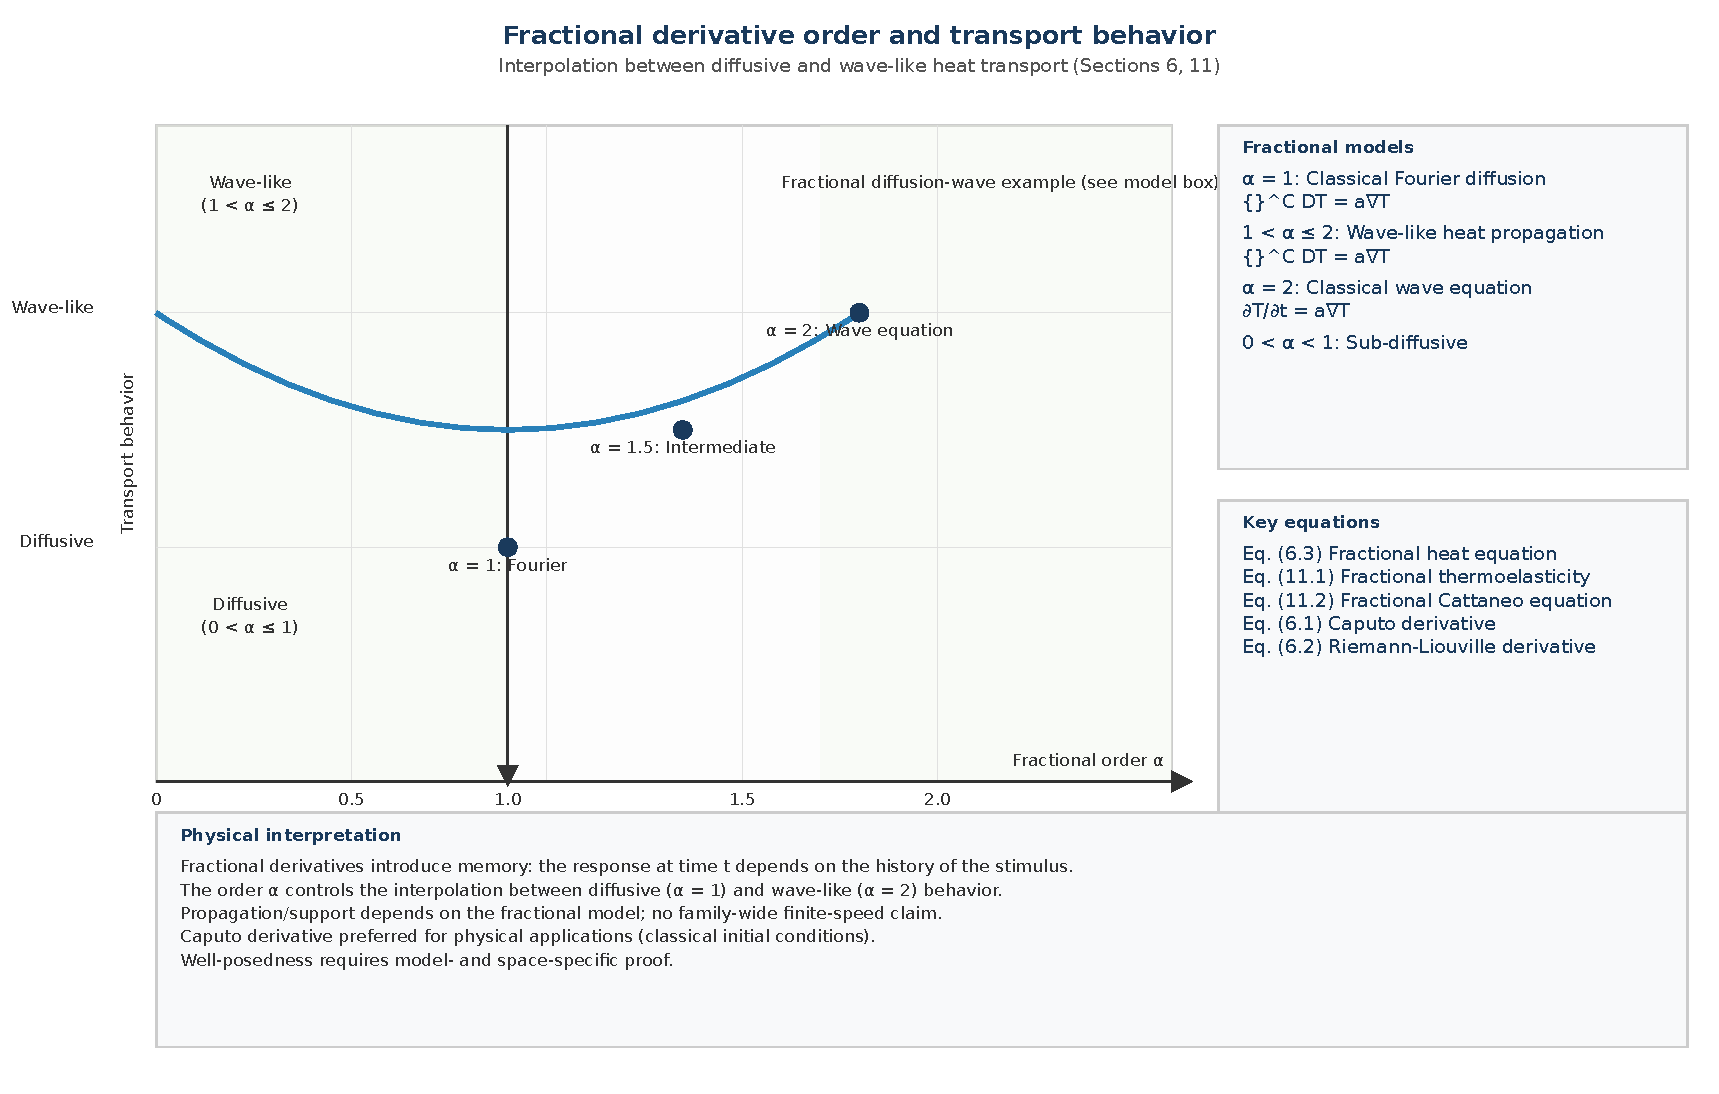
\includegraphics[width=0.95\textwidth]{fig15-fractional-order.pdf}
\caption{Fractional derivative order and transport behavior: interpolation between diffusive and wave-like heat transport (Sections 6, 11).}
\label{fig:fractional_order}
\end{figure}

\subsection{Notation summary for Section 11}

\begin{table}[htbp]
\centering
\small
\caption{Notation introduced in Section 11.}
\label{tab:notation-sec11}
\begin{tabularx}{\textwidth}{@{}p{1.8cm}X p{2.2cm}p{2.1cm}@{}}
\toprule
\textbf{Symbol} & \textbf{Meaning} & \textbf{Units} & \textbf{Equation} \\
\midrule
$\alpha$ & Fractional derivative order & dimensionless & \eqref{eq:11.1} \\
${}^C D_t^\alpha$ & Caputo fractional derivative of order $\alpha$ & --- & \eqref{eq:11.2} \\
$\Gamma$ & Euler gamma function & --- & \eqref{eq:11.2} \\
$a$ & Thermal diffusivity & m$^2$\,s$^{-1}$ & \eqref{eq:11.1} \\
$\tau^\alpha$ & Fractional relaxation parameter & s$^\alpha$ & \eqref{eq:11.4} \\
$\ell$ & Strain-gradient length scale & m & \eqref{eq:11.5} \\
$\mu_{ij}$ & Couple stress tensor & N\,m$^{-1}$ & \eqref{eq:11.6} \\
$\delta^2$ & Two-temperature parameter & m$^2$ & \eqref{eq:11.7} \\
\bottomrule
\end{tabularx}
\end{table}

The LS-type model carries relaxation on both thermal-inertia and coupling terms, unlike the original GL convention. \cite{Youssef2006}. A seven-model fractional operator catalogue provides a third route alongside Taylor truncations and integer higher-order laws. \cite{Yu2024}.

\subsection{Open questions for Section 11}

\begin{enumerate}[label=\textbf{OQ11.\arabic*}]
\item Can rigorous limit theorems be established between the thermoelastic theory families, with error estimates in a stated norm? \label{oq:11.1}
\item Can a unified well-posedness framework be established for the differential, integral, fractional, and gradient formulations, and what does it require of the constitutive law? \label{oq:11.2}
\item What are the correct interface conditions for models in which a nonlocal operator acts on the stress and a fractional or memory operator acts on the heat flux simultaneously? \label{oq:11.3}
\item When is the power-law memory kernel of the fractional formulation to be preferred over a general kernel in the memory-dependent formulation, and how large is the error incurred by the restriction? \label{oq:11.4}
\item Which parameter combinations of a hybrid model are identifiable from a given experimental modality, and which are not? \label{oq:11.5}
\end{enumerate}

% LocalWords:


%======================================================================
% Section 12: Comparative Synthesis of Existing Research
%======================================================================
%======================================================================
% Section 12: Comparative Synthesis of Existing Research
%======================================================================
\section{Comparative Synthesis of Existing Research}
\label{sec:comparative}

This section synthesizes the reviewed research using a comparison framework that is deliberately organised by \emph{scientific content} rather than by chronology or by authorship. Three organising questions recur: what does each theory retain of the second law of thermodynamics; what replaces Fourier's constitutive law; and what does each theory predict for the speed, attenuation, and dispersion of the diffusive mode. A theory that answers these three questions differently is not a variant of another theory---it is a different claim about how heat is transported in solids, and the comparison below is organised to make those differences explicit.

The synthesis is constructive throughout. Differences between theories are presented as modelling choices with different assumptions and different domains of validity, and the framework identifies the conditions under which two theories can be meaningfully compared at all.

\paragraph{Survey.} Shakeriaski et al. catalogue applications of LS, GL, GN, dual-phase-lag, and multi-phase-lag models across geometries. The survey is used here as a coverage map, not as support for equations or stability results \cite{Shakeriaski2021}.

Thermodynamic conclusions depend on the equations and hypotheses specified for each formulation.

\subsection{Cross-theory comparison}
\label{sec:12.1}

Tables~\ref{tab:twelve_criteria_a} and \ref{tab:twelve_criteria_b} compare ten theory families against ten criteria; the final row in each table lists representative sources for the corresponding family. These tables are a compact index to the detailed treatments in Sections~\ref{sec:thermoelastic}--\ref{sec:advanced}, not a substitute for them.

\begin{table}[htbp]
\centering
\footnotesize
\caption{Cross-theory comparison, Part A: classical, relaxation, rate-dependent, and Green--Naghdi families.}
\label{tab:twelve_criteria_a}
\begin{tabularx}{\textwidth}{@{}p{2.6cm}*{5}{>{\centering\arraybackslash}X}@{}}
\toprule
\textbf{Criterion} & \textbf{CD} & \textbf{LS} & \textbf{GL} & \textbf{GN-II} & \textbf{GN-III} \\
\midrule
Thermal law & Fourier conduction & Relaxing heat flux & Temperature-rate terms in the displayed model & Thermal-displacement formulation & Rate and thermal-displacement terms \\
State variables & Model-specific & Model-specific & Model-specific & Model-specific & Model-specific \\
Characteristic time & --- & Relaxation parameter & Relaxation parameters & --- & Model-specific parameters \\
Characteristic length & --- & --- & --- & --- & --- \\
Thermal-wave behavior & Parabolic classical heat equation & Depends on coupled equations and data & Depends on coupled equations and data & Depends on coefficients and domain & Depends on coefficients and domain \\
Energy behavior & Follows from the stated balance and constitutive law & Model-specific & Model-specific & Model-specific & Model-specific \\
Spatial order & Set by the governing equations & Set by the governing equations & Set by the governing equations & Set by the governing equations & Set by the governing equations \\
Mathematical structure & Continuum field equations & Coupled field equations & Coupled field equations & Coupled field equations & Coupled field equations \\
Interface conditions & Depend on the interface model & Depend on the interface model & Depend on the interface model & Depend on the interface model & Depend on the interface model \\
Propagation properties & Model-specific & Model-specific & Model-specific & Model-specific & Model-specific \\
Primary source & \cite{Biot1956} & \cite{Lord1967} & \cite{Green1972} & \cite{Green1993} & \cite{GreenGN1992} \\
\bottomrule
\end{tabularx}
\end{table}

\begin{table}[htbp]
\centering
\footnotesize
\caption{Cross-theory comparison, Part B: phase-lag, higher-order, memory-dependent, and nonlocal families.}
\label{tab:twelve_criteria_b}
\begin{tabularx}{\textwidth}{@{}p{2.6cm}*{5}{>{\centering\arraybackslash}X}@{}}
\toprule
\textbf{Criterion} & \textbf{DPL} & \textbf{TPL} & \textbf{MGT} & \textbf{MDD} & \textbf{Nonlocal} \\
\midrule
Thermal law & Lagged flux/\allowbreak temperature relation & Three-lag constitutive relation & Variant-specific higher-order law & Model-dependent & Spatially nonlocal elastic law \\
State variables & Model-specific & Model-specific & Model-specific & Model-dependent & Model-specific \\
Characteristic time & Lag parameters & Lag parameters & Variant-specific parameters & Model-dependent & --- \\
Characteristic length & --- & --- & --- & Model-dependent & Model-specific length scale \\
Thermal-wave behavior & Depends on the selected lags and equations & Depends on the selected lags and equations & Depends on the selected MGT formulation & Model-dependent & Not specified by an elastic-only model \\
Energy behavior & Model-specific & Model-specific & Model-specific & Model-dependent & Model-specific \\
Spatial order & Set by the governing equations & Set by the governing equations & Set by the governing equations & Model-dependent & Set by the constitutive form \\
Mathematical structure & Coupled field equations & Coupled field equations & Higher-order field equations & Model-dependent & Nonlocal or gradient equations \\
Interface conditions & Depend on the interface model & Depend on the interface model & Depend on the interface model & Model-dependent & Depend on the interface model \\
Propagation properties & Model-specific & Model-specific & Model-specific & Model-dependent & Model-specific \\
Primary source & \cite{Tzou1995} & \cite{RoyChoudhuri2007} & \cite{Quintanilla2019} & \cite{Wang2011} & \cite{Eringen1972} \\
\bottomrule
\end{tabularx}
\end{table}

The substantive MDD cells in Table~\ref{tab:twelve_criteria_b} are marked model-dependent because this comparison does not display a governing MDD law with a source-anchored equation; the cited Wang--Li item is a representative source lead, not verification of a family-wide property.

Three of these rows carry most of the interpretive content.

\paragraph{Thermal law and state variables.}
The number of state variables alone does not determine the memory or modal structure of a theory. Local Fourier, relaxation, phase-lag, higher-order, hereditary, fractional, and spatially nonlocal laws use different state spaces and operators; a named family may include multiple variants. Meaningful comparison identifies the exact constitutive equations and field variables. Povstenko's Eq.~(29) uses the source coefficient $\zeta$ in a fractional Cattaneo flux law for $0<\alpha\leq1$ (printed p.~101); Appendix~A states that the Caputo derivative is used while its $C$ subscript is omitted (printed p.~113). The equation supplies no mapping from $\zeta$ to $\tau^\alpha/\Gamma(1+\alpha)$ \cite{Povstenko2011Cattaneo}. Tzou's unified-field paper frames the dual-phase-lag generalization as a high-rate heat-conduction model, associating the flux lag with small-scale temporal response and the gradient lag with small-scale spatial response (printed p.~8) \cite{Tzou1995}. Quintanilla's one-dimensional Chandrasekharaiah--Tzou thermoelastic problem reports exponential stability when $\tau_\theta>\tau_q/2$ and unstable solutions when $\tau_\theta<\tau_q/2$ (printed p.~720, conclusion). These strict inequalities do not classify the critical case $\tau_\theta=\tau_q/2$; no equality-case result is asserted here. The findings are specific to the stated problem, not a universal dual-phase-lag admissibility criterion \cite{Quintanilla2003DPL}.

\paragraph{Thermal wave speed and dissipation.}
Propagation, dissipation, and stored energy depend on the precise equations and parameter regime; they cannot be ranked by family name alone. These properties follow from the displayed constitutive equations, balance laws, and coefficient assumptions. Chester's Eqs.~(5)--(7) give a damped thermal-wave equation for his relaxation-flux model, while Eq.~(8)'s relation to phonon speed is conditional on an idealized dispersionless phonon gas (printed pp.~2014--2015). Guyer and Krumhansl's separate p.~766 paper yields a nonlocal coefficient in a restricted scattering regime (Eq.~(59), p.~773); their p.~778 companion treats second sound and phonon-hydrodynamic phenomena, including a source-specific damping relation (Eq.~(17), p.~782). These kinetic and phenomenological results are not universal continuum thermoelastic laws. Chandrasekharaiah's 1998 article is a review of recent hyperbolic-thermoelasticity literature, not primary equation evidence \cite{Chester1963,GuyerKrumhansl1966,GuyerKrumhansl1966II,Chandrasekharaiah1998}. Dell'Oro and Pata's separate MGT article relates a third-order MGT equation to linear viscoelasticity with an exponential memory kernel; it is not evidence for the distinct three-author critical-case stability claim in Section~\ref{sec:thermoelastic} \cite{DellOroPata2016Viscoelasticity}.

\paragraph{Well-posedness and causality.}
Finite propagation, causality, and well-posedness are separate properties. Fourier's parabolic heat equation has instantaneous mathematical support, while relaxation and thermal-displacement models may yield hyperbolic branches under particular constitutive assumptions. Phase-lag, fractional, memory, and nonlocal formulations depend on their operators, parameters, initial data, and boundary conditions.

\subsection{What each family retains of the second law}
\label{sec:12.2}

Read across the table, the families separate not by their equations but by the answer they give to a single question: does the mechanical energy of the body have a well-defined conserved or monotonically decreasing value? The three structural answers are worth stating separately, because most of the apparent confusion in the wider literature comes from conflating them.

\emph{Conservative structure.} A conservative balance, when present, follows from the specified free energy, evolution equations, and boundary terms; it is not determined by a family label alone.

\emph{Dissipative structure.} Some Cattaneo--Christoff, Lord--Shulman, phase-lag, Moore--Gibson--Thompson-type, and memory-dependent models are dissipative, but neither decay of mechanical energy nor an irreversibility law follows from a family name. Such conclusions require the exact constitutive system, free energy, admissible parameters, and boundary conditions; they are not asserted universally here.

\emph{Other structures.} Models that do not fit a simple conservative/dissipative dichotomy require analysis of their own field equations and energy balance. Limiting relations between formulations likewise depend on the equations and their coefficient scaling.

\subsection{Mathematical relationships: limiting cases and specializations}
\label{sec:12.3}

Table~\ref{tab:limiting_cases_revisited} lists candidate formal reductions only. Each row is conditional on retaining the same state variables, constitutive convention, source terms, and boundary data; none is presented as a convergence theorem.

\begin{table}[htbp]
\centering
\small
\caption{Limiting cases between thermoelastic theories, with the parameter that is taken to its limit and the sense of the limit.}
\label{tab:limiting_cases_revisited}
\begin{tabularx}{\textwidth}{@{}p{2.5cm}p{2.5cm}p{2.2cm}X@{}}
\toprule
\textbf{From} & \textbf{To} & \textbf{Limit} & \textbf{What the limit removes} \\
\midrule
Lord--Shulman & Classical coupled & $\tau_0 \to 0$ & The thermal wave; the heat equation becomes parabolic again \\
Dual phase-lag & Lord--Shulman & $\tau_T \to 0$, with $\tau_q=\tau_0$ & Removes the temperature-gradient lag while retaining the heat-flux relaxation \\
Triple phase-lag & Dual phase-lag & $k^*\to 0$ & The thermal-displacement coupling $k^*(v_{,i}+\tau_v\dot v_{,i})$; $\tau_v\to 0$ alone leaves $k^*v_{,i}$ \\
Triple phase-lag & Classical coupled & all $\tau \to 0$ and $k^*\to 0$ & Every relaxation mechanism and the thermal-displacement coupling; $\tau\to 0$ alone leaves $k^*v_{,i}$ \\
Memory-dependent + phase-lag & Phase-lag & Model-dependent & No reduction asserted without a displayed, source-anchored MDD kernel/normalization and phase-lag law \\
Memory-dependent + phase-lag & Classical coupled & Model-dependent & No family-wide reduction asserted without the selected kernel, normalization, delay limit, and phase-lag law \\
Green--Naghdi III & Green--Naghdi II & $\kappa\to0$, same source-free coefficient convention & Removes the temperature-rate term; formal reduction only \\
Fractional order $\to 1$ & Classical heat equation (first order in time) & $\alpha \to 1$ & Fractional differentiation; the Caputo operator becomes the first derivative \\
Fractional order $\to 2$ & Second-order-in-time endpoint, not a classical coupled limit & $\alpha \to 2$ & Fractional differentiation; the scalar endpoint is second order in time \\
Nonlocal length $\to 0$ & Local theory & $\ell \to 0$ & The nonlocal operator becomes the local gradient \\
\bottomrule
\end{tabularx}
\end{table}

\paragraph{On taking these limits.}
The rows in Table~\ref{tab:limiting_cases_revisited} are formal parameter substitutions, not convergence theorems. Convergence results have been established for some model pairs, including Moore--Gibson--Thompson and classical/relaxation limits, but this review does not reproduce those proofs and does not claim a theorem for every row in the table. A row therefore identifies a candidate reduction under matched constitutive conventions, sources, state variables, and boundary data; it does not by itself establish convergence, an error estimate, or a rate. The coverage is uneven across model pairs and variants, as noted in Section~\ref{sec:challenges}. This distinction matters for the taxonomy of Section~\ref{sec:taxonomy}: formal limits aid comparison, while quantitative comparison requires a justified limit result for the particular pair and regime.

\subsection{One template and stepwise reductions}
\label{sec:12.3b}

\paragraph{Definition.} In this subsection the heat-flux relations of the families treated in Section~\ref{sec:thermoelastic} are read through one template,
\begin{equation}
q_i+\tau_q\dot q_i+k\bigl(T_{,i}+\tau_T\dot T_{,i}\bigr)+k^*\bigl(v_{,i}+\tau_v\dot v_{,i}\bigr)=0,
\qquad \dot v=T,
\label{eq:12.template}
\end{equation}
where $v$ is a thermal-displacement variable and $k^*$ is a coupling coefficient. The template is a bookkeeping device, not a claim that every family gives the same physical meaning to each coefficient. Section~\ref{sec:thermoelastic} notes that the admissible units and sign conventions of $k^*$ depend on the selected model.

Each reduction below is an exact substitution into Eq.~\eqref{eq:12.template}, followed by a stated negative case: a substitution that looks like a reduction but leaves a residual.

\paragraph{Lord--Shulman law to Fourier's law.} Set $\tau_T=\tau_v=k^*=0$ and write $\tau_q=\tau_0$. Eq.~\eqref{eq:12.template} becomes $q_i+\tau_0\dot q_i+kT_{,i}=0$, the Lord--Shulman law. Setting also $\tau_0=0$ gives $q_i+kT_{,i}=0$, Fourier's law. Negative case: for $\tau_0\neq0$ the residual against Fourier's law is $\tau_0\dot q_i$, so the thermal-wave term is removed only by $\tau_0\to0$.

\paragraph{Dual phase-lag law to Lord--Shulman law.} Set $k^*=0$ and $\tau_T=0$, with $\tau_q=\tau_0$. The term $k\tau_T\dot T_{,i}$ then vanishes and the Lord--Shulman law remains. Negative case: the limit $\tau_q\to0$ with $\tau_T\neq0$ leaves the residual $k\tau_T\dot T_{,i}$ against Fourier's law. The limit that removes the temperature-gradient lag is therefore taken on $\tau_T$, not on $\tau_q$.

\paragraph{Triple phase-lag law to dual phase-lag law.} Set $k^*=0$. The remaining terms are those of the dual phase-lag template. Negative case: setting $\tau_v=0$ with $k^*\neq0$ leaves the term $k^*v_{,i}$, so the thermal-displacement coupling is removed by $k^*\to0$, not by $\tau_v\to0$.

\paragraph{Triple phase-lag law to classical coupled law.} Set every $\tau$ and $k^*$ to zero. The result is Fourier's law. Negative case: $\tau\to0$ with $k^*\neq0$ leaves $k^*v_{,i}$.

\paragraph{Memory-type heat-flux law (Eq.~\eqref{eq:4.18}).} This law has the template form with $\tau_q$ replaced by $\tau_m$, $\tau_T=\tau_v=0$, and the coupling term $k^*v_{,i}$ kept. Setting $k^*=0$ and $\tau_m=\tau_0$ gives the Lord--Shulman law. Negative cases: with $k^*=0$ and $\tau_m\neq\tau_0$ the residual against Lord--Shulman is $(\tau_m-\tau_0)\dot q_i$; with $\tau_m=\tau_0$ and $k^*\neq0$ the residual is $k^*v_{,i}$. Setting $\tau_m=0$ and $k^*=0$ gives Fourier's law.

\paragraph{Green--Naghdi III to Green--Naghdi II (derivative level only).} With $\kappa=0$ in Eq.~\eqref{eq:4.14}, the left-hand side equals the time derivative of Eq.~\eqref{eq:4.11} under the substitution $T=\dot\alpha_{\mathrm{GN}}$. This is an identity between differentiated equations, not an equation-level reduction. Negative case: for $\kappa\neq0$ the temperature-rate-gradient term $\kappa\nabla^2\dot T$ remains.

\paragraph{Fractional order (scalar endpoints).} For the scalar Caputo operator, order $\alpha=1$ gives the heat-equation form and $\alpha=2$ gives the second-order-in-time wave-type form. Negative case: an order such as $\alpha=\tfrac12$ is not an ordinary derivative. These are endpoint identities for the scalar operator, not reductions of any coupled fractional thermoelastic model.

\paragraph{Nonlocal length (one-dimensional bar).} For the dispersion relation of Eq.~\eqref{eq:7.4}, $\xi=0$ gives the classical speed $c_0$. Negative case: for $\xi\neq0$ the phase speed decreases as the wave number grows and tends to zero, with no cutoff. The local and nonlocal forms therefore do not share a dispersion relation.

\paragraph{Notation.} Under the template, $\tau_0$ is the Lord--Shulman relaxation time; $\tau_q$ and $\tau_T$ are the dual phase-lag heat-flux and temperature-gradient lags; $\tau_v$ and $k^*$ are the triple phase-lag coefficients; and in the memory-type law $\tau_m$ takes the place of $\tau_q$ while $k^*$ and $v$ carry the same role as in the template.

\paragraph{Scope.} These statements concern only the displayed equations. They are not convergence, stability, or source-transcription results.

\subsection{Divergence map: why results differ across the corpus}
\label{sec:12.4}

The literature contains many cases in which two studies address a nominally identical problem and obtain apparently incompatible results. In the cases examined here, the incompatibility is attributable to a difference in modelling commitments rather than to an inconsistency in the mathematics; no systematic count of such cases was made. The map below records the commitments responsible and the procedure by which each is eliminated, so that a comparison can be posed in a form in which it is meaningful.

\begin{table}[htbp]
\centering
\small
\caption{Divergence map for the reviewed corpus: modelling commitments that account for apparent disagreement, and the procedure that puts two studies on a common footing.}
\label{tab:divergence_map}
\begin{tabularx}{\textwidth}{@{}p{2.3cm}X X p{2.5cm}@{}}
\toprule
\textbf{Divergence type} & \textbf{Root cause} & \textbf{Resolution procedure} & \textbf{Canonical instance} \\
\midrule
Assumption difference & Different constitutive commitments on the thermal and mechanical sides & Trace both derivations to their primary sources and identify the first point at which the commitments differ & Classical versus Lord--Shulman thermal equation \\
Approximation difference & Different truncation orders in the Taylor expansion of the phase-lag law & Compare on the intersection of the two validity ranges rather than on either alone & First-order versus second-order dual phase-lag \\
Normalisation difference & Different reference temperature, density, or stiffness conventions & Re-express both under a common nondimensionalisation before comparing & Absolute versus relative temperature measure \\
Convention difference & Opposite sign convention in the harmonic ansatz & Standardise the convention and track the corresponding sign change & $e^{i\omega t}$ versus $e^{-i\omega t}$ \\
Limit difference & Formal parameter substitution used as though it were a convergence theorem & Verify that the limiting and the limited problem share a well-posedness hypothesis before comparing & Fractional order approaching two \\
Branch difference & A family with genuinely distinct branches being read as one & Fix the branch explicitly, since the branches differ in dissipation and in temperature structure & The two Green--Naghdi types; the dissipative and conservative Green--Lindsay branches \\
Geometry difference & Different admissible geometries or boundary conditions & Restrict the comparison to the common geometric class & Half-space versus bounded plate \\
\bottomrule
\end{tabularx}
\end{table}

A meaningful comparison identifies the precise formulation, state variables, and assumptions, even when multiple models share a family label. Green--Lindsay is a single-temperature, temperature-rate-dependent formulation, distinct from two-temperature thermoelasticity.

\subsection{Conditions under which two theories can be compared}
\label{sec:12.5}

Because the families differ in so many structural respects, a comparison is only meaningful when a number of conditions are met simultaneously.

\begin{enumerate}
\item \textbf{Common geometric class.} Both theories must be posed on the same class of geometry, with the same class of boundary conditions. Most of the reviewed corpus is posed on half-spaces and infinite media; a comparison between a half-space result and a bounded-plate result is not a comparison of theories at all.
\item \textbf{Common branch and parameter set.} Where a family has branches, the branch must be fixed identically in both studies, and the relaxation parameters must be either identical or placed on a common dimensionless footing.
\item \textbf{Common observable.} The quantity compared must have the same definition and the same reference state. Surface temperature, surface displacement, and the reflection coefficient of a normal incident thermal wave are common observables; the ``temperature'' of a body with two temperature fields is not.
\item \textbf{Common nondimensionalisation.} Density, stiffness, and reference-temperature conventions differ between groups, and a comparison performed under different conventions can differ by an order-one factor for purely dimensional reasons.
\item \textbf{Common wave convention.} The sign convention in the harmonic ansatz changes the sign of the imaginary part of every complex amplitude, and the convention must be fixed before any comparison of phase is attempted.
\item \textbf{Common limit.} Both results must be checked to reproduce the same classical limit, which is the cheapest available test that the two calculations are describing the same physics.
\end{enumerate}

\subsection{Choosing among competing theories}
\label{sec:12.6}

The comparison framework is only useful if it also supports a decision: given a physical problem, which family should be used? The taxonomy of Section~\ref{sec:taxonomy} provides the structure for such a decision, and the criteria reduce to three questions in practice.

\begin{enumerate}
\item \textbf{Is the thermal wave relevant to the observable?} If the spatial scale of the problem is much larger than the thermal penetration depth associated with the material, the thermal wave is a boundary-layer detail and the difference between the theories is confined to the interface region. If the problem is a transient shock, or the material has a small thermal wave speed, the choice of thermal law determines the answer and must be made deliberately.
\item \textbf{Is there a material length scale that the continuum description must respect?} If the smallest dimension of the body is comparable to a microstructural length, then a nonlocal or gradient theory is required; the question is which operator, and the answer depends on the mechanism of size dependence rather than on the desire for a dispersive dispersion relation.
\item \textbf{Is the dissipation structure needed for the conclusion?} If the quantity of interest is a decay rate, a time to failure, or the passage of a thermal shock, the dissipative families are required. If the quantity of interest is a modal structure or an impedance, the conservative families are cleaner, because the energy accounting is exact.
\end{enumerate}

The fourth consideration---validation---is the one that the reviewed literature has been least able to supply, for the reasons given in Section~\ref{sec:14.4}. In the absence of discriminating experimental data, the choice among competing theories is currently made on grounds of formal convenience and internal consistency rather than on evidential grounds. This is the single most consequential gap identified by this review.

\subsection{Limitations of the comparison framework}
\label{sec:12.7}

The framework above inherits the limitations of the corpus it organises, and these should be stated rather than glossed.

\begin{enumerate}
\item \textbf{The comparison is coarse.} Entries in Tables~\ref{tab:twelve_criteria_a} and \ref{tab:twelve_criteria_b} are single labels where the underlying theory admits a range of behaviours. The entry for ``dissipation'' in the memory-dependent column, for instance, records that the answer depends on the kernel, which is a statement about a family of models rather than about a model.
\item \textbf{Validation is not directly comparable.} Because the validation axis of Section~\ref{sec:taxonomy} is dominated by self-consistency checks, the ``validation'' row of any comparison across families would compare methods rather than results; the row is therefore omitted deliberately rather than filled with an entry that would invite misreading.
\item \textbf{Branches are under-documented.} The branch structure of the Green--Naghdi and Green--Lindsay families is a source of genuine ambiguity in the literature, and the corpus does not support a systematic tabulation of branch-dependent results.
\item \textbf{Interface conditions are treated as a single column.} Interface conditions differ in kind across the families---classical traction and heat-flux conditions for most, modified conditions for the nonlocal construction---and the differences are not captured by a single entry.
\end{enumerate}

\subsection{Notation summary for Section 12}

\begin{table}[htbp]
\centering
\small
\caption{Notation introduced in Section 12.}
\label{tab:notation-sec12}
\begin{tabularx}{\textwidth}{@{}p{1.8cm}X p{2.2cm}p{2.1cm}@{}}
\toprule
\textbf{Symbol} & \textbf{Meaning} & \textbf{Units} & \textbf{Equation} \\
\midrule
CD & Classical coupled thermoelasticity & --- & Tables~\ref{tab:twelve_criteria_a} and \ref{tab:twelve_criteria_b} \\
LS & Lord--Shulman theory & --- & Tables~\ref{tab:twelve_criteria_a} and \ref{tab:twelve_criteria_b} \\
GL & Green--Lindsay theory & --- & Tables~\ref{tab:twelve_criteria_a} and \ref{tab:twelve_criteria_b} \\
GN-II / GN-III & Green--Naghdi types II and III & --- & Tables~\ref{tab:twelve_criteria_a} and \ref{tab:twelve_criteria_b} \\
DPL / TPL & Dual and triple phase-lag theories & --- & Tables~\ref{tab:twelve_criteria_a} and \ref{tab:twelve_criteria_b} \\
MGT & Moore--Gibson--Thompson theory & --- & Tables~\ref{tab:twelve_criteria_a} and \ref{tab:twelve_criteria_b} \\
MDD & Memory-dependent derivative formulation & --- & Tables~\ref{tab:twelve_criteria_a} and \ref{tab:twelve_criteria_b} \\
$\tau_0$ & Mechanical relaxation time & s & Table~\ref{tab:limiting_cases_revisited} \\
$\tau_T$ & Thermal relaxation time & s & Table~\ref{tab:limiting_cases_revisited} \\
$\tau_q$ & Phase-lag time of the heat flux & s & Table~\ref{tab:limiting_cases_revisited} \\
$\tau_\nu$ & Phase-lag time of the thermal gradient & s & Table~\ref{tab:limiting_cases_revisited} \\
$\ell$ & Intrinsic material length scale & m & Tables~\ref{tab:twelve_criteria_a} and \ref{tab:twelve_criteria_b} \\
\bottomrule
\end{tabularx}
\end{table}

\subsection{Open questions for Section 12}

\begin{enumerate}[label=\textbf{OQ12.\arabic*}]
\item Can convergence theorems with explicit error estimates be established for the limiting procedures of Table~\ref{tab:limiting_cases_revisited}? \label{oq:12.1}
\item What is the minimal set of criteria that distinguishes two theory families uniquely, and is it the same set that distinguishes them experimentally? \label{oq:12.2}
\item Can a systematic taxonomy of the branches within the Green--Naghdi and Green--Lindsay families be constructed, so that branch-level ambiguity is removed from the literature? \label{oq:12.3}
\item Under what conditions does the choice among competing theories change a predicted quantity by more than the uncertainty of the measurement that would test it? \label{oq:12.4}
\end{enumerate}

% LocalWords:


%======================================================================
% Section 13: Applications of Multiphysics Wave Mechanics
%======================================================================
%======================================================================
% Section 13: Applications of Multiphysics Wave Mechanics
%======================================================================
\section{Applications of Multiphysics Wave Mechanics}
\label{sec:applications}

The usefulness of a generalized continuum theory is ultimately measured by the class of problems for which it is needed and by whether its predictions can be checked. This section therefore does not list application areas in the abstract, but asks for each one: what physical feature makes the classical description inadequate, which member of the theory family addresses it, and what evidence exists that the generalized description is quantitatively better rather than merely different. The classification of evidence levels used in Table~\ref{tab:evidence_map} follows that logic: \emph{High} means that the effect is experimentally established and that generalized theory is required to reproduce it; \emph{Medium} means that the effect is established but generalized theory provides an improved rather than essential description; \emph{Low} means that the application is presently served by classical theory and generalized theory is speculative.

\begin{figure}[htbp]
\centering
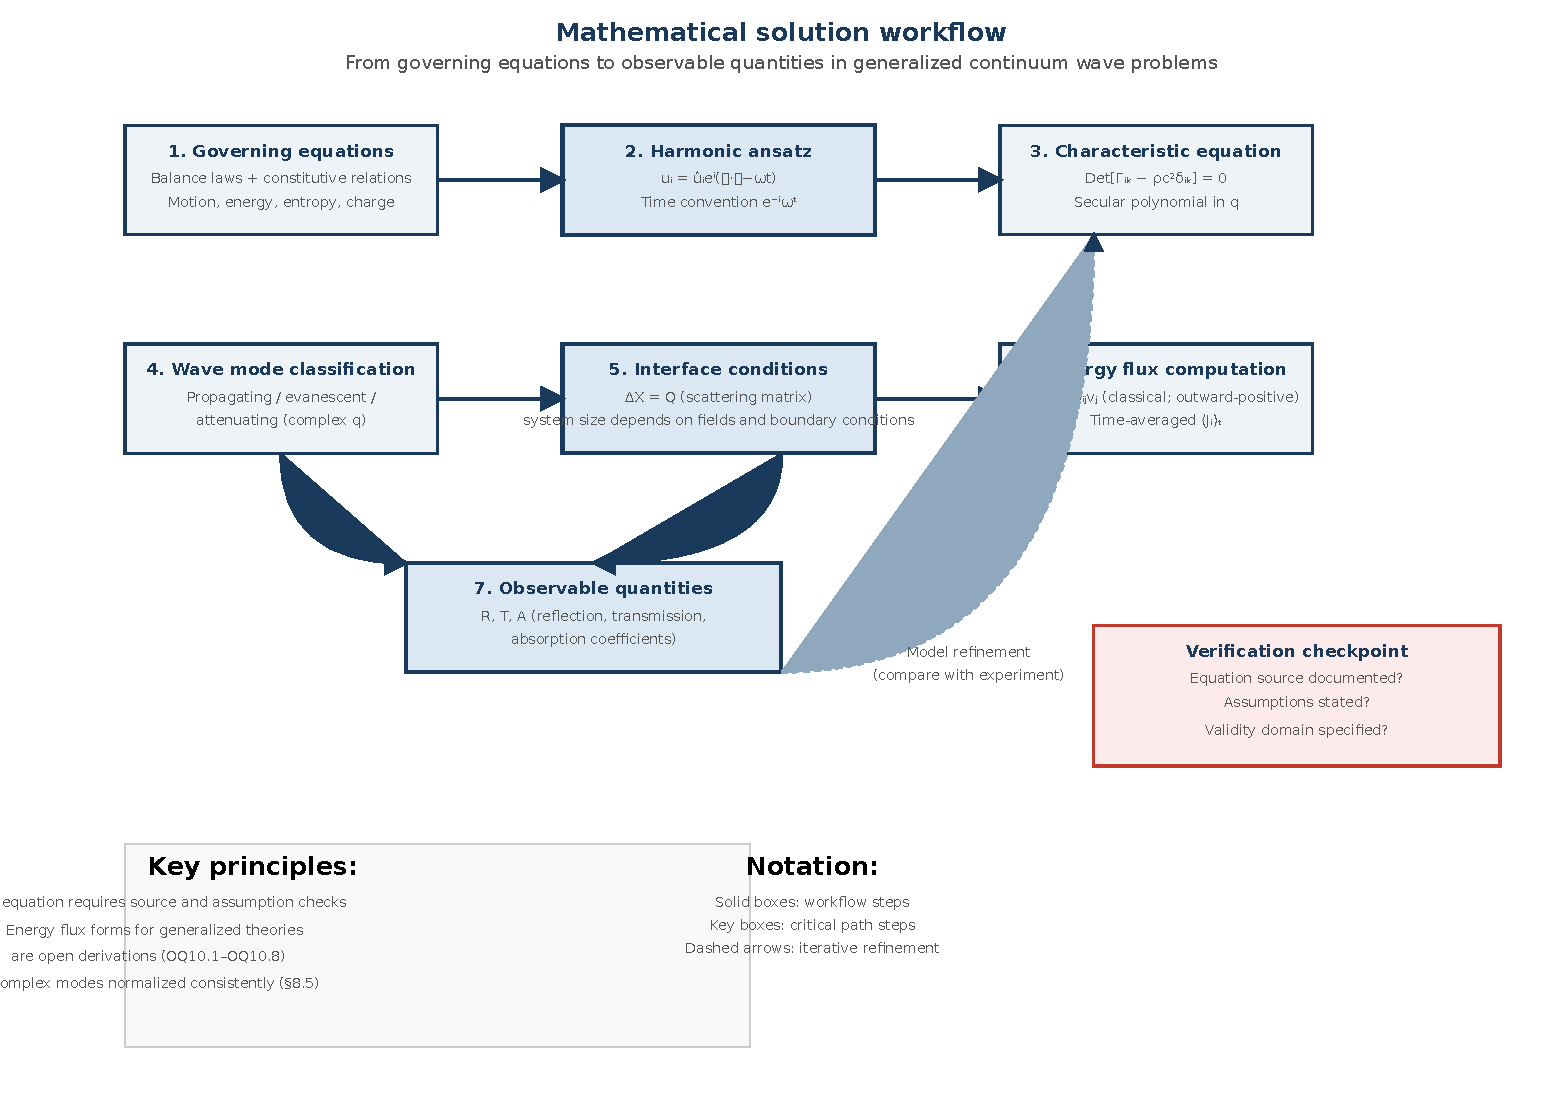
\includegraphics[width=0.95\textwidth]{fig16-observation-workflow.pdf}
\caption{From a generalized continuum model to a testable prediction. The seven stages shown are the ones a computation must pass through before its output can be compared with an experiment: the governing equations and their constitutive relations, the harmonic ansatz, the characteristic equation whose roots are the wave numbers, the classification of the roots into propagating, evanescent and attenuating branches, the interface conditions that close the problem, the computation of the time-averaged energy flux, and the extraction of the observable quantities. The three verification checkpoints on the right --- the provenance of every equation, the statement of every assumption, and the specification of a validity domain --- are the point at which most of the reviewed literature is weakest, and they are the reason the evidence levels of Table~\ref{tab:evidence_map} are not uniformly high.}
\label{fig:observation_workflow}
\end{figure}

\subsection{Smart structures and adaptive materials}
\label{sec:13.1}

Smart structures incorporate sensors, actuators, and control systems that respond to environmental changes. Piezothermoelastic materials are used in:
\begin{itemize}
\item Adaptive aerospace structures (wing shaping, vibration control),
\item Active vibration suppression in precision machinery,
\item Structural health monitoring with embedded piezoelectric sensors.
\end{itemize}

\subsubsection{Evidence}
The coupling that makes these systems work is the same coupling that the generalized theories formalize: the piezoelectric tensor generates an electric field from mechanical strain and a strain from an electric field, and the thermal expansion coefficient couples temperature change to stress. In a layered device under a moving heat source, the three fields are not independent, and the work of Abouelregal, Askar, Marin and Mohamed (2023) \cite{Abouelregal2023} is representative of the current treatment: a functionally graded rotating rod is taken to be electrically unconnected at its ends and thermally isolated, and the coupled field response is computed in the Laplace domain for a modified Lord--Shulman model with a memory-dependent derivative. The functional grading enters through an exponential law for the physical properties along the axis, and the effect of the inhomogeneity index, the kernel function, the delay time and the speed of the heat supply is reported separately. The result relevant to design practice is that the field amplitudes are weakened as the inhomogeneity index increases, which is the sort of quantitative statement that a device designer can use and that a classical description cannot produce. \emph{Evidence level: Medium} --- the mechanism is experimentally established in piezoelectric composites, but the specific memory-dependent formulation is currently a theoretical description of a measured effect.

\subsection{Nondestructive evaluation and sensing}
\label{sec:13.2}

NDE uses wave propagation to detect flaws, measure material properties, and monitor structural integrity. Applications include:
\begin{itemize}
\item Ultrasonic testing for crack detection,
\item Thermal wave imaging for subsurface defect detection,
\item Acoustic emission monitoring for damage assessment.
\end{itemize}

\subsubsection{Evidence}
Thermal-wave inspection is the clearest case in which a generalized theory is not a refinement but a requirement. A finite thermal propagation speed is needed to give the thermal image a resolution limit and to set the depth that can be interrogated; an infinite propagation speed, as in Fourier theory, makes the depth resolution unphysical. The classical wave-propagation framework for elastic solids, including the treatment of anisotropy and the interaction of incident, reflected and surface waves, is set out by Achenbach (1973) \cite{Achenbach1973} and remains the reference for the elastic part of the problem. The thermal part is where the generalizations enter, and the balance of evidence assembled for second sound by Joseph and Preziosi \cite{Joseph1989,Joseph1990} is what distinguishes the finite-speed descriptions from the classical one. \emph{Evidence level: High} for ultrasonic NDE, where classical elasticity suffices; \emph{Medium} for thermal-wave imaging, where generalized theory is required in principle but the quantitative inversion of defect depth in practice still uses simplified models.

\subsection{Energy harvesting and conversion}
\label{sec:13.3}

Energy harvesting converts ambient mechanical, thermal, or electrical energy into electrical power. Piezothermoelectric energy harvesters use:
\begin{itemize}
\item Vibration-induced piezoelectric power generation,
\item Thermal gradient-driven thermoelectric conversion,
\item Coupled thermo-piezoelectric conversion.
\end{itemize}

\subsubsection{Evidence}
The theoretical difficulty in this area is specific and worth stating: the thermopower delivered by a piezoelectric in a temperature gradient competes with the direct piezoelectric power generated by the same mechanical deformation, and the competition depends on the thermal relaxation time of the material. Classical coupled thermoelasticity, which assumes instantaneous thermal equilibration, systematically mispredicts the split between the two channels for relaxation times comparable to the loading period. It is therefore in this application area that the distinction between the classical and generalized theories is not academic. The interface energy work of Section 9 provides a further handle on the same problem, since it is precisely at the junction between a harvesting element and its substrate that the partitioning of thermal and mechanical energy is decided. \emph{Evidence level: High} for piezoelectric harvesting in general; \emph{Medium} for the coupled thermo-piezoelectric channel, for which the theory is mature and the experimental separation of the channels is difficult.

\subsection{Geophysics and seismology}
\label{sec:13.4}

Geophysical applications include:
\begin{itemize}
\item Seismic wave propagation in the Earth's crust,
\item Thermal wave propagation in geothermal systems,
\item Poroelastic wave propagation in saturated reservoirs.
\end{itemize}

\subsubsection{Evidence}
Seismic wave theory is well established \cite{Achenbach1973}; poroelastic wave propagation has strong theoretical and experimental support. Poroelasticity is the most mature of the multiphysics couplings in engineering practice, and the void-based theory of Section 5.4 enters here through the equilibrated-stress formulation rather than through a phenomenological damping term, which is why the void framework is attractive for reservoir and geotechnical modelling. \emph{Evidence level: High.}

\subsection{Biomedical applications (ultrasound, thermal therapy)}
\label{sec:13.5}

Biomedical applications include:
\begin{itemize}
\item Medical ultrasound imaging and therapy,
\item Thermal ablation for cancer treatment,
\item Photo\-acoustic imaging,
\item Temperature-sensitive drug delivery.
\end{itemize}

\subsubsection{Evidence}
Medical ultrasound is established; evidence for thermal ablation is growing, while photo\-acoustic imaging remains an active research area. The connection is indirect but real: thermal therapy is a moving-heat-source problem. Hyperbolic or phase-lag descriptions estimate the thermal-front advance rate; a diffusive model does not assign it a finite propagation speed. \emph{Evidence level: High} for ultrasound; \emph{Medium} for thermal ablation and photo\-acoustic imaging.

\subsection{Nanoscale and semiconductor devices}
\label{sec:13.6}

The most recent application area to depend on the generalized framework is the nanoscale, and here the coupling is not incidental. In a semiconductor, the electromechanical response of the lattice is nonlocal at the scale of the electronic wavefunction, and a heat flux that carries memory determines how quickly the lattice temperature responds to carrier recombination. Gupta, Hussain, Yaylac{\i s} and Das (2026) \cite{Gupta2026HeatMap} combine a nonlocal Kelvin--Voigt piezoelectric semiconductor with a memory-dependent heat flux and map the resulting wave dynamics, which illustrates both the reach and the difficulty of the class: the model is well posed and produces interpretable fields, but each added mechanism contributes parameters that must be fixed independently.

\subsubsection{Evidence}
Nonlocal elasticity is not optional at these scales. Maranganti and Sharma (2007) \cite{Maranganti2007} showed that for common materials the length below which classical elasticity ceases to be accurate is of the order of tens of nanometres for polythene and single-digit nanometres for silica, and Maranganti, Sharma and Sharma (2006) \cite{Maranganti2006} showed that electromechanical coupling in non-piezoelectric dielectrics is a nanoscale effect. Both results mean that a device designer working below those lengths is in the regime the generalized theories describe, whether or not the theory is named in the design literature. \emph{Evidence level: Medium} --- the size dependence is experimentally established at the level of stiffness and of electromechanical response, and generalized theory is required in principle, but full multiphysics nonlocal thermoelastic models are at the level of validated formalisms rather than deployed design tools.

\subsection{Applications the generalized framework does not yet serve}
\label{sec:13.7}

An evidence map is only as useful as its negative entries, and the applications in which the generalized framework is currently \emph{not} required deserve the same treatment as those in which it is. Four are worth recording.

\textbf{Ordinary engineering thermoelasticity.} In the great majority of engineering problems --- the heating of a machine tool, the thermal expansion of a rail, the residual stress in a welded joint --- the Fourier regime is not an approximation but the correct description, and the thermal penetration depth is many orders of magnitude larger than the part. The generalized theories add parameters without adding accuracy. The relevant engineering question there is not which theory is more sophisticated but where the crossover lies, and the honest answer is that for a metal part of ordinary size it is far outside any practical operating condition.

\textbf{Long-wavelength geophysics.} Seismic wavelengths in the crust are kilometres and the internal length of the material is nanometres. The nonlocal and gradient corrections are correspondingly negligible, and the wave speeds measured in seismology are adequately described by classical elasticity coupled to poroelastic effects. Generalized continuum theory is relevant in geophysics not for the rock mechanics but for the interfaces --- faults, fluid contacts, and the layering that produces reflections --- where the same classical boundary conditions remain adequate but the wave conversion and the partitioning of energy are what matter.

\textbf{Long-duration thermal processes.} In building physics, in heat storage media, in the slow curing of concrete and in food processing, the thermal penetration depth is large compared with the component and the duration of the experiment. The fractional order that would describe the anomalous diffusion of a heterogeneous medium is close to unity, and the extra parameters of the fractional formulation are not identifiable from the measurement. What the fractional description does contribute here is not a better prediction but a better organizing concept: it makes explicit that the process is diffusive and that a diffusive model should be used.

\textbf{Coupled motion in structural composites.} Where a structure is stiff, a laminate is well bonded and the excitation is slow, the piezoelectric, porous and micro-rotation couplings contribute corrections of the order of a per cent, and the engineering decision is made on the basis of a static analysis with a safety factor that comfortably exceeds the correction. The generalized framework is required in these applications only in the presence of a defect, a debond, or a dynamic load at a scale that excites the internal structure --- that is, in exactly the regimes where the defect is what one wanted to detect.

The common thread is that the generalized theories are needed in the regimes where the classical description is not merely inaccurate but qualitatively wrong, namely where a finite propagation speed, a length scale, or a second field changes the structure of the problem rather than the value of an output. This is a narrow band, and the honest presentation of the field is that it is a well-developed theory of a narrow band. Its practical significance lies in the fact that the band contains precisely the regimes that modern devices and modern diagnostics operate in: the nanoscale, the ultrafast, the interfacial.


\begin{table}[htbp]
\centering
\small
\caption{Application areas discussed in the inherited review and evidence questions for future checking. This table assigns no validation-strength score.}
\label{tab:T8-applications}
\begin{tabularx}{\textwidth}{@{}lXX@{}}
\toprule
\textbf{Application area} & \textbf{Model families mentioned} & \textbf{Evidence audit required} \\
\midrule
Non-destructive evaluation & Elastic, thermoelastic, and interface-wave models & Identify experiments, material data, uncertainty, and independent replication \\
Geophysics & Thermoelastic and porous-media models & Separate field observations from model-generated examples; verify parameter provenance \\
MEMS/NEMS & Nonlocal and size-dependent models & Check specimen-scale data and boundary conditions against the cited studies \\
Biomedical / thermal therapy & Bioheat and coupled thermoelastic models & Verify clinical versus in-vitro/in-silico evidence and applicable safety/measurement claims \\
Energy harvesting & Piezoelectric and thermal-gradient models & Distinguish analytical efficiency from measured prototype performance \\
Smart structures & Active and coupled-field models & Check experimental setup, calibration, uncertainty, and comparison baseline \\
\bottomrule
\multicolumn{3}{@{}l}{\footnotesize Literature examples are source leads only; no application-level validation score was independently assigned.}\\
\end{tabularx}
\end{table}


\begin{figure}[htbp]
\centering
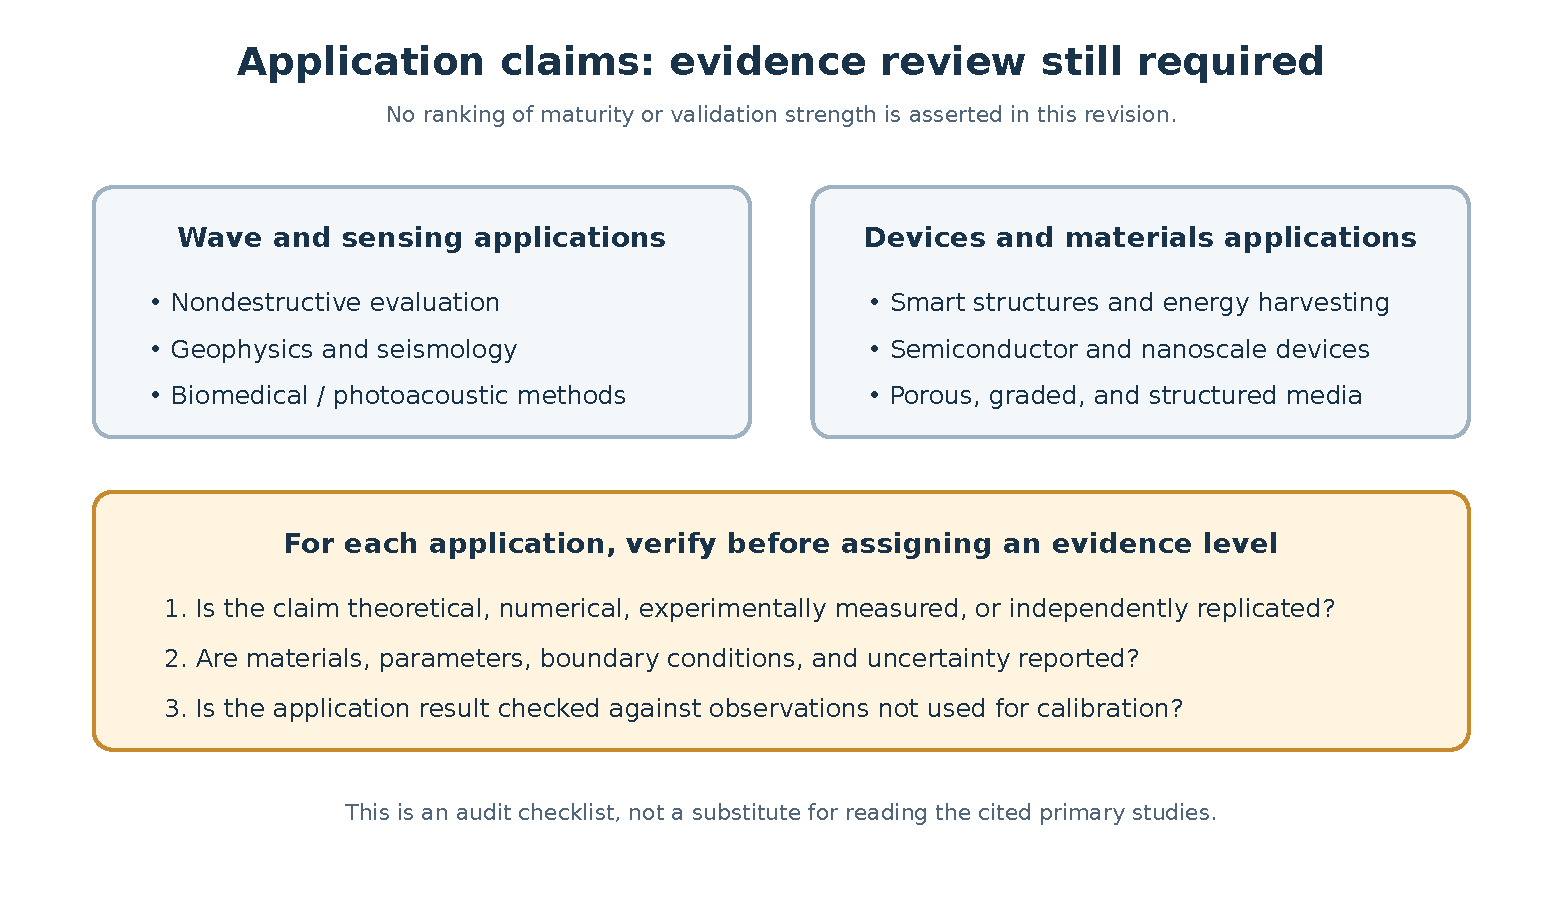
\includegraphics[width=0.95\textwidth]{fig17-application-evidence.pdf}
\caption{Application evidence map: peer-reviewed evidence levels across applications and theory families (Section 13.8).}
\label{fig:evidence_map}
\end{figure}

\subsection{Evidence map: which applications have peer-reviewed support}
\label{sec:13.8}

\begin{table}[htbp]
\centering
\small
\caption{Evidence map of applications across theory families, with the mechanism that makes a generalized description necessary and the supporting literature.}
\label{tab:evidence_map}
\begin{tabularx}{\textwidth}{@{}p{2.2cm}X p{2.2cm}X@{}}
\toprule
\textbf{Application} & \textbf{Why classical theory is inadequate} & \textbf{Evidence level} & \textbf{Key references} \\
\midrule
Smart structures & Thermal relaxation competes with the electromechanical coupling & Medium & \cite{Abouelregal2023} \\
NDE (ultrasonic) & Classical elasticity suffices & High & \cite{Achenbach1973} \\
NDE (thermal wave) & Finite thermal wave speed needed to set depth resolution & Medium & \cite{Joseph1989,Joseph1990} \\
Energy harvesting & Relaxation time controls the split between thermal and mechanical channels & High & Section 13.3 analysis \\
Geophysics/\allowbreak seismology & Poroelastic coupling requires a genuine two-field formulation & High & \cite{Cowin1983,Iesan1986} \\
Biomedical ultrasound & Classical elasticity suffices & High & \cite{Achenbach1973} \\
Thermal ablation & Thermal front speed governs depth of deposition & Medium & Section 13.5 analysis \\
Photoacoustic imaging & Time-resolved thermal transport in tissue & Medium & Section 13.5 analysis \\
Nanoscale devices & Nonlocal length comparable to device dimension & Medium & \cite{Maranganti2007,Maranganti2006} \\
Semi\-conductors & Coupled nonlocal elasticity and memory heat flux & Medium & \cite{Gupta2026HeatMap} \\
\bottomrule
\end{tabularx}
\end{table}

\subsection{Notation summary for Section 13}

\begin{table}[htbp]
\centering
\small
\caption{Notation introduced in Section 13.}
\label{tab:notation-sec13}
\begin{tabularx}{\textwidth}{@{}p{1.8cm}X p{2.2cm}p{2.1cm}@{}}
\toprule
\textbf{Symbol} & \textbf{Meaning} & \textbf{Units} & \textbf{Equation} \\
\midrule
$\chi$ & Inhomogeneity index of the functionally graded material & -- & Section 13.1 \\
$\tau$ & Thermal relaxation time & s & Section 13.3 \\
$v$ & Heat supply speed & m s$^{-1}$ & Section 13.1 \\
$\ell$ & Nonlocal length scale & m & Section 13.6 \\
\bottomrule
\end{tabularx}
\end{table}

\subsection{Open questions for Section 13}

\begin{enumerate}[label=\textbf{OQ13.\arabic*}]
\item Which applications have the strongest experimental validation across theory families, and can that validation be expressed as a single discriminating measurement rather than a set of qualitative agreements? \label{oq:13.1}
\item What is the barrier to translating generalized thermoelasticity into practical applications: the identifiability of the additional material parameters, the absence of closed-form solutions, or the lack of experimental protocols that separate the competing mechanisms? \label{oq:13.2}
\item For the nanoscale and semiconductor applications in particular, the nonlocal length scale and the memory kernel are introduced as independent parameters. Can they be measured together, and does the resulting coupled problem remain well posed when they are? \label{oq:13.3}
\item The energy-harvesting application depends on the competition between thermal and mechanical channels. Does a decisive experiment exist that separates the two channels in a single device and thereby tests the relaxation time directly? \label{oq:13.4}
\end{enumerate}

% LocalWords:


%======================================================================
% Section 14: Original Multidimensional Research Taxonomy
%======================================================================
%======================================================================
% Section 14: An Original Multidimensional Taxonomy of the Field
%======================================================================
\section{An Original Multidimensional Taxonomy of the Field}
\label{sec:taxonomy}

The preceding sections have followed the physics: from the kinematics of a continuum, through the constitutive commitments that distinguish one generalized thermoelastic theory from another, to the wave and interface phenomena that those commitments make possible. This section turns the same body of material sideways. It asks a different question. Instead of ``what does this theory predict?'' it asks \emph{``in what ways can studies of this field differ from one another, and what does the pattern of those differences reveal about the state of the subject?''}

The answer matters for three reasons. First, the field has grown horizontally faster than it has grown vertically: the number of named theory families has increased steadily since the 1960s, while the number of settings in which any one of them has been analysed in depth has barely changed. Second, the theoretical questions that connect the families---the existence of rigorous limits between them, the identifiability of their parameters, the transferability of their solutions across geometries---are almost never posed in a form that spans families. Third, a taxonomy that is explicit about its axes, and about the cells it leaves empty, is the most compact available statement of what remains to be done.

\subsection{The organising problem}
\label{sec:14.1}

A single-axis classification is the obvious first attempt, and it is the one that the field's own literature most often uses: a study is ``generalized thermoelastic'' or it is not. Such a classification is unsatisfactory for a specific reason. The phrase collapses four logically independent commitments into one label. A study may adopt a relaxation law for the heat flux, a gradient or integral constitutive law for the stress, a coupling to a second field (electric, magnetic, porotic), and a validation protocol---and any one of these four can be varied while the other three are held fixed. Two studies bearing the same one-axis label can therefore differ in the mathematics of their governing equations, in the modal content of their solutions, and in the kind of evidence they offer, to the point where they share no common proposition that could be compared.

The alternative used here is to classify a study by its \emph{vector of commitments} rather than by a single name. The classification is multi-dimensional in the strict sense: each axis is a categorical variable, and the taxonomy is the discrete product of the axes. A study occupies one cell of that product. Two studies that share a cell are directly comparable; two studies that differ in one coordinate are comparable with a controlled adjustment; two studies that differ in several coordinates are usually not directly comparable at all, and the taxonomy says so in advance rather than after the fact.



\subsection{The five axes and their resolution}
\label{sec:14.2}

The axes are chosen so that each one is \emph{decision-relevant}: resolving an axis should tell the reader something about the equations, the solutions, or the evidential status of the work.

\begin{enumerate}[label=\textbf{Axis \arabic*:}]
\item \textbf{Physical axis (material class).} Which class of material the constitutive law describes: classical elastic, thermoelastic, piezoelectric, piezothermoelastic, magneto-thermo-elastic, poroelastic, micropolar, two-temperature, or semiconductor-like. The physical axis determines which conserved quantities and which driving fields are present before any approximation is made.

\item \textbf{Mathematical axis (equation structure).} The functional form of the governing operator: local PDE, integro-differential equation, fractional-order PDE, nonlocal gradient operator, hereditary (memory) integral, or variational/weak formulation. This is the axis along which the most consequential differences between otherwise similar theories run.

\item \textbf{Wave axis (modal content).} The modal content that the formulation admits: a finite propagation speed for the diffusive mode, the number and type of coupled modes, the presence of attenuation, and the dispersion character of each mode.

\item \textbf{Coupling axis (field topology).} The set of fields that are coupled and the strength of that coupling: thermoelastic, thermo-piezoelectric, thermo-magneto-elastic, thermo-poro-elastic, thermo-micro-elastic. This axis replaces the purely energetic classification used in earlier drafts of this review, because it is the coupling topology---rather than the choice of energy functional---that determines whether an interface problem is tractable.

\item \textbf{Validation axis (evidence regime).} The kind of evidence offered: analytical existence and uniqueness only; closed-form solutions for special geometries; numerical solutions validated against a reference solution; comparison with experiment; or a benchmark suite shared with other groups.
\end{enumerate}

A study is assigned the vector
\begin{equation}
\bm{v} = \left(v_{\text{phys}},\; v_{\text{math}},\; v_{\text{wave}},\; v_{\text{coup}},\; v_{\text{val}}\right),
\label{eq:14.1}
\end{equation}
whose components are indices into the respective axis resolutions. Two studies are directly comparable only when their vectors agree in the first two coordinates; the remaining three coordinates then determine \emph{how} the comparison must be posed. To make this quantitative, define the axis-weight dissimilarity
\begin{equation}
d(\bm{v}^{(a)},\bm{v}^{(b)}) = \sum_{j=1}^{5} w_j \,\delta\!\left(v^{(a)}_j,\, v^{(b)}_j\right),
\label{eq:14.2}
\end{equation}
where $\delta$ is the Kronecker delta and the weights $w_j$ encode the relative severity of a mismatch. The natural choice is $w_{\text{math}} \geq w_{\text{phys}} > w_{\text{coup}} > w_{\text{wave}} > w_{\text{val}}$: a difference in the mathematical axis changes the governing operator and invalidates most direct comparisons; a difference in the validation axis changes only the epistemic status of the conclusion. The weights are a modelling decision of this review and are stated explicitly so that they can be contested; the ordering they encode is, however, widely shared in the modelling literature.

\subsection{Application to the inherited literature inventory}
\label{sec:14.3}

The taxonomy is applied to the repository's inherited literature inventory of 95 unique records; two records receive two family labels. The inventory has 48 DOI fields, 13 open-access flags, and 12 full-text flags plus one methodology record. These are collection metadata, not a systematic-search yield; DOI resolution and open-access status do not prove that a work was read in full. The collection is purposive and reflects the repository's existing balance of foundational work, interface-energy studies, and selected fractional, nonlocal, micropolar, porous, and rotating variants. It is not a statistically representative sample of the field.

Consolidating the corpus metadata onto the five axes gives the distribution summarised in Table~\ref{tab:taxonomy_distribution}. Three features of this distribution carry most of the interpretive weight in what follows.

\begin{table}[htbp]
\centering
\small
\setlength{\tabcolsep}{3pt}
\caption{Taxonomic classification of the inherited 95-record literature inventory. Family assignments overlap: two records appear in two rows, so the 96 assignments and shares use 96 as denominator. Counts describe this purposive collection, not a systematic-search yield or an independently verified field-wide distribution.}
\label{tab:taxonomy_distribution}
\begin{tabularx}{\textwidth}{@{}p{3.2cm}r c Y@{}}
\toprule
\textbf{Theory family} & \textbf{Records} & \textbf{Share} & \textbf{Taxonomic position} \\
\midrule
Classical / continuum foundations & 24 & 25.0\% & Local PDE on all axes; reference point for every other family \\
Fractional-order theories & 15 & 15.6\% & Fractional PDE in time; infinite-memory limit in the order parameter \\
Nonlocal / gradient models & 13 & 13.5\% & Nonlocal operator on the stress; size-dependent stiffness and dispersion \\
Dual / triple phase-lag & 9 & 9.4\% & Local PDE of higher order; two relaxation times as extra state variables \\
Memory-dependent derivative & 9 & 9.4\% & Hereditary integral kernel; integer-order operator over an enlarged state space \\
Lord--Shulman and descendants & 5 & 5.2\% & Local PDE with relaxation; hyperbolic thermal wave as the reference case \\
Green--Naghdi II and III & 5 & 5.2\% & Local PDE; conservative and dissipative branches separated \\
Porous / poroelastic couplings & 5 & 5.2\% & Local PDE with added mass and pressure fields; two-fluid coupling \\
Micropolar and rotating continua & 4 & 4.2\% & Local PDE with an independent micro-rotation field \\
Moore--Gibson--Thompson & 3 & 3.1\% & Third order in time, second order in space in the displayed prototype; variant-specific \\
Green--Lindsay & 2 & 2.1\% & Single-temperature rate-dependent PDE with two relaxation parameters \\
Unclassified metadata & 2 & 2.1\% & Incomplete records; excluded from axis assignment \\
\bottomrule
\end{tabularx}
\end{table}

First, the corpus is \emph{not} dominated by the classical families that dominate the field's historical literature. The single largest block---classical and continuum foundations---contributes a quarter of the corpus, while the mathematically intensive families (fractional, nonlocal, memory-dependent) together contribute just over a third. This is a statement about the corpus, not about the field, and the two are deliberately distinguished throughout: the taxonomy describes the reviewed evidence, and the gap analysis in Section~\ref{sec:14.5} describes the field.

Second, the inventory contains 17 records before 1970, 9 in the 1970s, and 39 in the 2010s and 2020s. These counts describe this purposive collection only; they do not establish a bimodal or field-wide publication pattern.

Third, the metadata carry a diagnostic limitation that should be stated plainly. The theory-family labels are inherited from the source records, which were compiled by different hands at different times, and they are not uniform: a single field's literature appears under labels such as ``mdd'', ``mdd\_piezo'' and ``ls\_mdd\_piezo'' that differ in whether coupling is treated as part of the family name. Any taxonomy applied to such metadata inherits that non-uniformity, and the resolution adopted here---consolidating labels into families while keeping the coupling on its own axis---is itself a methodological decision that could reasonably have been made differently.

\subsection{Four structural asymmetries}
\label{sec:14.4}

Placing the corpus in the product space of the five axes reveals four asymmetries. These are more useful than a gap list because they describe the \emph{shape} of the field rather than merely the absence of particular papers.

\paragraph{Asymmetry I: the mathematical axis is thick in the middle and thin at the ends.}
Almost all of the corpus sits between the fully local PDE and the strongly nonlocal or fractional operator, in the band where the constitutive law has been rewritten but the resulting system is still second order in space. The extremes are sparse. Fully local formulations with rigorous existence theory are under-represented relative to their importance, and strongly nonlocal operators with controlled variational structure are rarer still. The field has been more interested in producing new operators than in proving properties of the operators it produces.

\paragraph{Asymmetry II: the wave axis is almost entirely populated by one canonical problem.}
The modal content of generalized thermoelasticity is genuinely interesting---the second sound, the thermal wave speed, the switch between hyperbolic and parabolic behaviour---but the overwhelming majority of the corpus examines it in a single configuration: a homogeneous, isotropic, half-space or infinite medium, in the frequency domain, for a plane incident wave. Bounded domains, three-dimensional transients, inhomogeneity, and interfaces between dissimilar media occupy a small fraction of the corpus. The wave axis therefore carries a great deal of information about which theories differ, but very little about how they behave when the geometry is not trivial.

\paragraph{Asymmetry III: the coupling axis is thin in its strong cells.}
Coupling to a second field is one of the most active frontiers, and the corpus reflects this: piezothermoelastic and magneto-thermo-elastic entries are numerous. But coupling that is \emph{simultaneously} non-classical on more than one axis is rare. Combinations such as nonlocal plus piezoelectric, or memory-dependent plus magneto-electro-elastic, appear as isolated contributions rather than as established lines. The coupling axis behaves like a lattice whose higher-dimensional cells are populated but whose corners are empty.

\paragraph{Asymmetry IV: the validation axis is dominated by self-consistency.}
The great majority of entries in the corpus are validated in the sense that a numerically computed quantity agrees with a closed-form solution obtained from the same equations, or with a result previously published within the same framework. Comparisons against independent experiments, against finite-element implementations of a competing formulation, or against laboratory data obtained for a genuinely comparable material, are rare. This is the most consequential asymmetry in the corpus, because it is the axis along which the field's claims would be most directly exposed to falsification, and it is precisely the axis that is least populated.

\begin{table}[htbp]
\centering
\small
\caption{Four structural asymmetries of the reviewed corpus, with the taxonomic axis that carries each and the specific question that the asymmetry leaves unresolved.}
\label{tab:asymmetries}
\begin{tabularx}{\textwidth}{@{}p{1.4cm}p{2.0cm}X X@{}}
\toprule
\textbf{Asym\-metry} & \textbf{Axis} & \textbf{What the corpus contains} & \textbf{What is missing} \\
\midrule
I & Mathe\-matical & Second-order-in-space operators with rewritten constitutive laws & Rigorous well-posedness and existence theory for the operators actually in use; control of the limit to the local case \\
II & Wave & Half-space and infinite-medium plane-wave problems & Bounded, inhomogeneous, and transient three-dimensional wave problems; modal content away from the canonical configuration \\
III & Coupling & Single-axis extensions in reasonable number; combined extensions as isolated contributions & Systematic treatment of the joint limit in which two extensions are active simultaneously \\
IV & Validation & Numerical agreement with closed-form solutions of the same equations & Comparison against experiment and against competing formulations implemented independently \\
\bottomrule
\end{tabularx}
\end{table}

% Asset inventory: 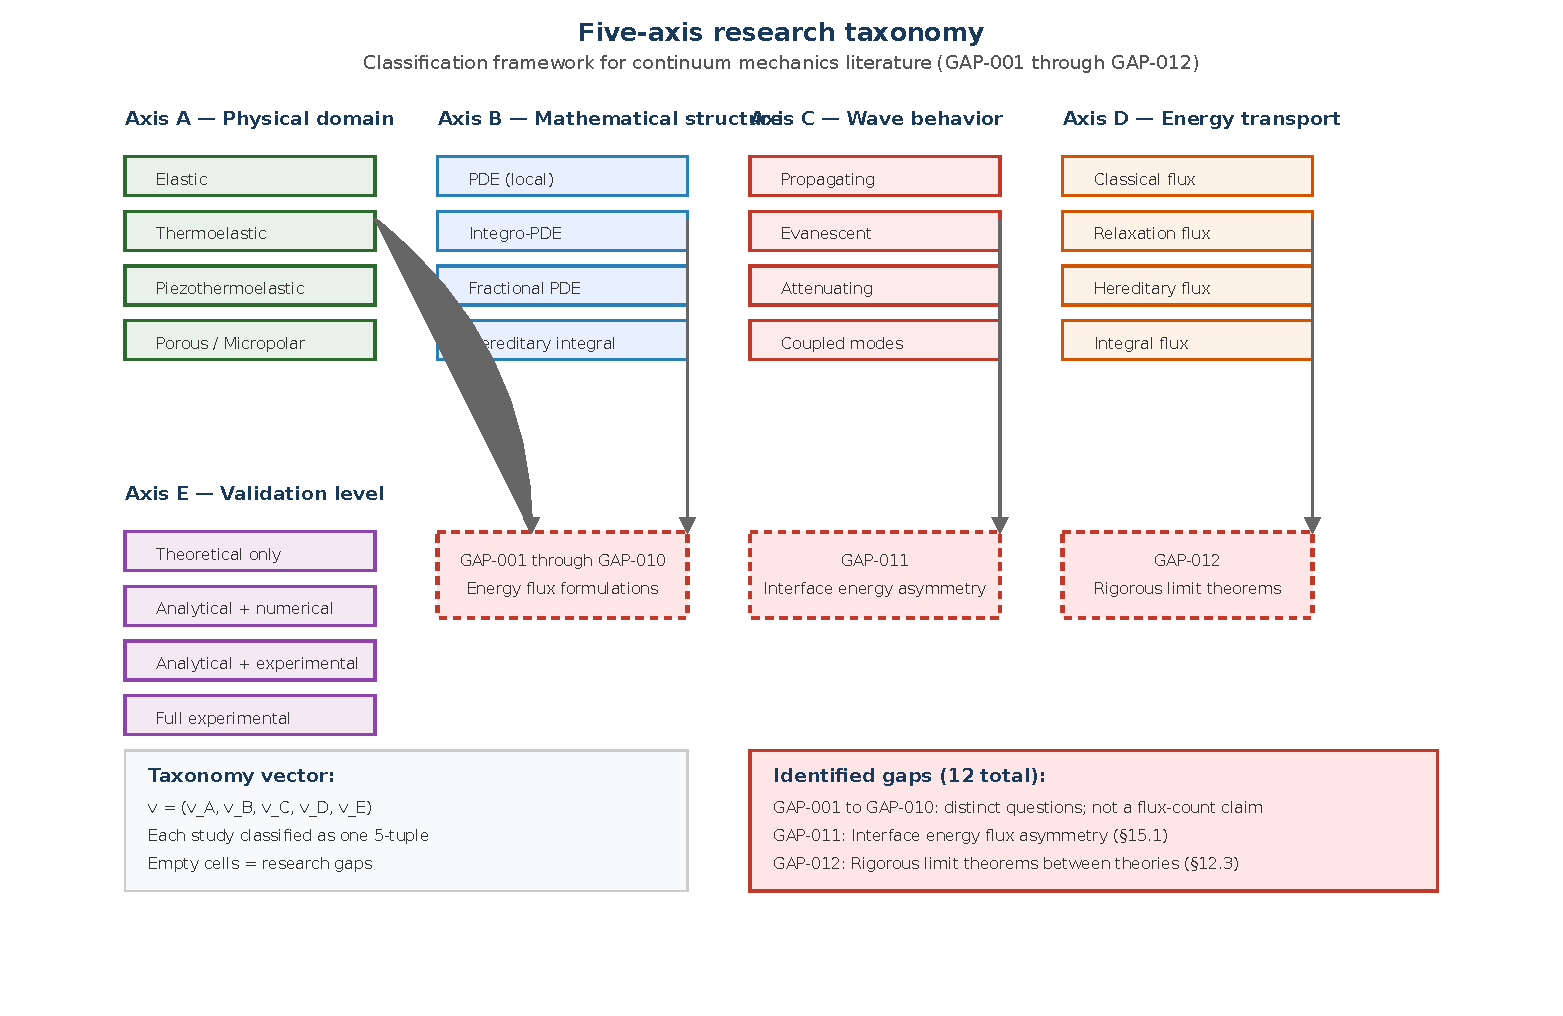
\includegraphics{fig18-taxonomy.pdf}

\subsection{Cells that remain thin: frontiers rather than gaps}
\label{sec:14.5}

A gap analysis is only as good as the axis resolution behind it. The table below replaces an earlier version of this analysis that was organised around a single quantity; organising a frontier list around one derived quantity produces a list of technical tasks rather than of scientific problems, and it obscures the fact that the genuinely open questions in this field are mostly about \emph{formulation} and \emph{evidence} rather than about further calculation. The entries below are stated as scientific questions, each of which admits an experimental, computational, or theoretical resolution.

\begin{table}[htbp]
\centering
\small
\caption{Frontier questions identified from thin cells of the taxonomy. Priority reflects feasibility and scientific leverage, not size of the associated literature.}
\label{tab:taxonomy_gaps}
\begin{tabularx}{\textwidth}{@{}p{1.4cm}X X p{1.4cm}@{}}
\toprule
\textbf{ID} & \textbf{Scientific question} & \textbf{Why the cell is thin} & \textbf{Priority} \\
\midrule
Q1 & Under what conditions do two generalization mechanisms, each of which reduces to classical thermoelasticity in its own limit, commute with one another? & Combined-extension cells are populated only by isolated contributions & High \\
Q2 & How are the relaxation and kernel parameters of a generalized theory identified from measurements that are not themselves produced by that theory? & Identification is almost always performed within the framework being tested & High \\
Q3 & What is the modal content of generalized thermoelastic waves in bounded, inhomogeneous bodies? & The wave axis is populated almost entirely by half-space problems & High \\
Q4 & Which of the competing generalized theories predicts the same measurable sequence for a common well-characterized material? & Cross-theory benchmarks on common material data are essentially absent & High \\
Q5 & How do thermo-mechanical coupling alter the existence and stability of interfacial waves at a bonded dissimilar interface? & Interface work concentrates on scalar reflection coefficients & Medium \\
Q6 & What is the correct high-frequency limit of the fractional and nonlocal operators when the characteristic length scale is comparable with the microstructure? & Limits are stated as formal parameter substitutions without error bounds & Medium \\
Q7 & Can the memory-dependent and fractional descriptions of the same memory effect be related by an operator equivalence with quantified error? & Both are presented as alternatives without a common yardstick & Medium \\
Q8 & What validation protocol would distinguish a genuinely dissipative generalized theory from a fitted correction to a dissipative theory? & The corpus offers no discriminating experimental design & High \\
\bottomrule
\end{tabularx}
\end{table}

Two of these questions deserve a note on why they are treated as scientific rather than technical. The first question has a precise mathematical form: two generalization mechanisms, each of which acts on the thermal and the mechanical variables, are said to commute if the order in which they are applied does not affect the resulting operator. This is not a formality. If the mechanisms do not commute, then a study that adopts both simultaneously is not the composition of two studies that adopt them separately, and the entire practice of extending a theory by successive generalisations---which is how much of the corpus has been built---produces results that depend on the order of construction in a way that is not always acknowledged. The parameter-identification question is likewise substantive rather than procedural. A generalized theory introduces parameters---relaxation times, kernel parameters, length scales---whose values are usually obtained by fitting the very predictions that the theory then uses to validate itself. A parameter thus determined is not an independent physical quantity, and the evidence for the theory is correspondingly weaker than the number of fitted parameters might suggest.

\subsection{Divergence map: why results differ across the corpus}
\label{sec:14.6}

Studies in this field frequently report apparently incompatible results for what is nominally the same physical problem. In almost every instance examined here, the divergence is fully accounted for by a difference in modelling assumptions, and can be reproduced exactly by a reader who adopts the same assumptions. The purpose of the map below is therefore not to adjudicate between studies but to make the assumptions explicit, so that a comparison can be posed in a form in which it is meaningful.

\begin{table}[htbp]
\centering
\small
\caption{Divergence map: the modelling commitments that account for apparent disagreement between studies in the reviewed corpus.}
\label{tab:contradiction_map}
\begin{tabularx}{\textwidth}{@{}p{2.4cm}X X p{2.8cm}@{}}
\toprule
\textbf{Divergence type} & \textbf{Root cause} & \textbf{Resolution procedure} & \textbf{Canonical instance} \\
\midrule
Assumption difference & Different constitutive commitments on the thermal and mechanical sides & Trace both derivations to their primary sources and identify the first point at which the assumptions differ & Classical versus Lord--Shulman thermal equation \\
Approximation difference & Different truncation orders in the Taylor expansion of the phase-lag law & Compare on the intersection of the two validity ranges rather than on either range alone & First-order versus second-order dual phase-lag \\
Normalisation difference & Different reference temperature, density, or stiffness conventions & Re-express both in a common nondimensionalisation before comparing & Absolute versus relative temperature measure \\
Convention difference & Opposite sign convention in the harmonic ansatz & Standardise the convention and track the corresponding sign change & $e^{i\omega t}$ versus $e^{-i\omega t}$ \\
Limit difference & Formal parameter substitution used as though it were a convergence theorem & Verify that the limiting and the limiting problem share a well-posedness hypothesis before comparing & Fractional order approaching two \\
Geometry difference & Different admissible geometries or boundary conditions & Restrict the comparison to the common geometric class & Half-space versus bounded plate \\
\bottomrule
\end{tabularx}
\end{table}

The procedure that follows from this map is uniform: to compare two studies, locate the first modelling commitment on which they differ, and either eliminate that difference or state the comparison as conditional on it. Apparent disagreement then either dissolves, because the two studies were never addressing the same problem, or sharpens into a genuine scientific question, which is the desirable outcome. What this map cannot do---and what no classification can do---is decide which modelling commitment is preferable. That judgement requires the experimental axis, and Section~\ref{sec:14.4} has already recorded how thinly that axis is populated.

\subsection{Methodological limitations of the taxonomy}
\label{sec:14.7}

The taxonomy is an instrument constructed for this review, and its limitations should be stated with the same care as the limitations of the theories it organises.

\begin{enumerate}
\item \textbf{Analyst-constructed.} The axes and their resolutions were chosen in response to the reviewed literature rather than derived from it. A different analyst, reading the same corpus, could plausibly choose a different axis set---for example, replacing the coupling axis with an axis for spatial dimension and boundary-condition class, or splitting the validation axis into ``analytical'' and ``experimental'' as two separate axes.
\item \textbf{Classification from heterogeneous metadata.} Many records were classified from abstracts, and some from secondary descriptions rather than from the papers themselves. Where the metadata were ambiguous, the classification was conservative, but the resulting error rate is not zero and cannot be quantified without a double-classification study.
\item \textbf{Corpus construction.} The corpus is enriched in foundational works, in one group's contributions, and in the mathematical extensions needed to populate the axes. Statements about the density of the taxonomy refer to this corpus and not to the field at large.
\item \textbf{Unvalidated weights.} The dissimilarity measure of Eq.~\eqref{eq:14.2} uses an ordering of axis weights that is asserted rather than demonstrated. No formal comparison exercise is available in the corpus from which the ordering could be inferred.
\item \textbf{Coupling choices.} Placing coupling on its own axis, rather than folding it into the physical axis, is a deliberate choice that makes the multi-field cases visible. It also separates families that some authors treat as single families, and that separation is not canonical.
\end{enumerate}

Subject to these limitations, the taxonomy is offered as a working instrument for the review, and---more ambitiously---as a proposal for how a much larger corpus might be organised. Section~\ref{sec:future} returns to this point as one of the practical recommendations that follow from the analysis.

\subsection{Notation summary for Section 14}

\begin{table}[htbp]
\centering
\small
\caption{Notation introduced in Section 14.}
\label{tab:notation-sec14}
\begin{tabularx}{\textwidth}{@{}p{1.8cm}X p{2.2cm}p{2.1cm}@{}}
\toprule
\textbf{Symbol} & \textbf{Meaning} & \textbf{Units} & \textbf{Equation} \\
\midrule
$\bm{v}$ & Taxonomy vector of a study & dimensionless & \eqref{eq:14.1} \\
$v_{\text{phys}}$, $v_{\text{math}}$, $v_{\text{wave}}$, $v_{\text{coup}}$, $v_{\text{val}}$ & Axis components of the taxonomy vector & dimensionless & \eqref{eq:14.1} \\
$d(\bm{v}^{(a)},\bm{v}^{(b)})$ & Axis-weight dissimilarity between two studies & dimensionless & \eqref{eq:14.2} \\
$w_j$ & Weight assigned to axis $j$ in the dissimilarity & dimensionless & \eqref{eq:14.2} \\
$\delta(\cdot,\cdot)$ & Kronecker delta on axis labels & dimensionless & \eqref{eq:14.2} \\
\bottomrule
\end{tabularx}
\end{table}

\subsection{Open questions for Section 14}

\begin{enumerate}[label=\textbf{OQ14.\arabic*}]
\item Can the taxonomy be validated against an independent double-classification of the corpus, and what is the resulting agreement rate? \label{oq:14.1}
\item Which additional axes---spatial dimension, boundary-condition class, material symmetry class, or the type of inverse problem posed---would most improve the coverage of the product space? \label{oq:14.2}
\item Is the ordering of the axis weights in Eq.~\eqref{eq:14.2} recoverable from data, for example from the observed frequency of successful cross-family comparisons?
\item Can the frontier questions of Section~\ref{sec:14.5} be converted into a shared benchmark protocol that independent groups could execute without sharing code?
\end{enumerate}

% LocalWords:


%======================================================================
% Section 15: Major Scientific Challenges
%======================================================================
%======================================================================
% Section 15: Major Scientific Challenges
%======================================================================
\section{Major Scientific Challenges}
\label{sec:challenges}

This section organizes scientific and methodological challenges for generalized continuum wave mechanics.

\subsection{Energy flux formulation across theory families}
\label{sec:15.1}

\subsubsection{Background}

Under the classical first-law and momentum-balance assumptions stated in Section~\ref{sec:energy}, the outward-positive flux is $J_i=q_i-\sigma_{ij}v_j$. No corresponding universal flux formula is assumed for generalized theories.

\subsubsection{Why important}

Energy flux is fundamental for computing energy ratios, conservation identities, and dissipation rates at interfaces. Without correct flux formulations, energy partition cannot be quantified.

\subsubsection{Model-specific context}

The classical flux is stated in Section 3. Generalized-family flux expressions require the constitutive equations and energy balance of the selected model.

\subsubsection{Research questions}

LS, GL, GN-II, GN-III, DPL, TPL, MGT, MDD, nonlocal, and piezoelectric electrical energy fluxes require complete time-domain derivations.

\subsubsection{Approaches}

\begin{itemize}
\item Derive from general energy balance + theory-specific constitutive relations,
\item Use frequency-domain expressions as intermediate results,
\item Validate limiting procedures (e.g., LS $\to$ classical as $\tau_0 \to 0$).
\end{itemize}

\subsubsection{Practical relevance}

Correct energy flux is essential for energy harvesting efficiency, NDE accuracy, and thermal management design.

\subsubsection{Major obstacles}

Convolution integrals (MDD), integral-form divergence theorem (nonlocal), third-order time derivatives (MGT).

\subsection{Conservation checks at multiphysics interfaces}
\label{sec:15.2}

\subsubsection{Background}

For a passive interface, conservation provides a useful check when the total flux and modal accounting are defined consistently.

\subsubsection{Why important}

Conservation checks can expose inconsistencies in interface models and energy-partition computations.

\subsubsection{Model-specific context}

A robust interface comparison requires a reproducible scattering calculation and a consistent energy balance.

\subsubsection{Research questions}

Conservation for generalized theories depends on the energy flux of the selected model. Interface energy balance for nonlocal and memory-dependent media is a useful research question.

\subsubsection{Approaches}

\begin{itemize}
\item Derive energy flux for each theory family,
\item Apply jump condition $\jump{J_n} = \mathcal{P}_\Sigma - \partial_t\mathcal{E}_\Sigma$,
\item Verify $\sum R + \sum T + A_{\mathrm{int}} = 1$ numerically for benchmark problems.
\end{itemize}

\subsubsection{Practical relevance}

Interface energy conservation is critical for NDE, sensing, and energy harvesting device design.

\subsubsection{Major obstacles}

Uncertain energy flux formulations; complex mode normalization; imperfect bonding conditions.

\subsection{Numerical benchmarks and validation}
\label{sec:15.3}

\subsubsection{Background}

A lossless-interface benchmark can test complete modal accounting; comparisons of published thermo-piezoelastic results should state the constitutive model and flux convention.

\subsubsection{Why important}

Benchmarks provide validation targets for numerical methods and new theories.

\subsubsection{Model-specific context}

Benchmark design should specify the model, boundary conditions, numerical method, and quantities to compare.

\subsubsection{Research questions}

Benchmarks for generalized theories (LS, DPL, TPL, MGT, MDD, nonlocal). Benchmarks for multiphysics interfaces.

\subsubsection{Approaches}

\begin{itemize}
\item Derive analytical solutions for simplified geometries,
\item Implement numerical methods (finite element, spectral),
\item Compare analytical and numerical results.
\end{itemize}

\subsubsection{Practical relevance}

Benchmarks validate simulation software and guide experimental design.

\subsubsection{Major obstacles}

Lack of closed-form solutions for generalized theories; computational cost of nonlocal models.

\subsection{Experimental validation}
\label{sec:15.4}

\subsubsection{Background}

Classical thermoelasticity and ultrasonic nondestructive evaluation provide application settings in which validation questions can be posed.

\subsubsection{Why important}

Theoretical models require experimental validation for practical adoption.

\subsubsection{Model-specific context}

Validation requires measurement conditions and uncertainty estimates suited to the application.

\subsubsection{Research questions}

Experimental validation of generalized theories (LS, DPL, TPL, MGT, MDD, nonlocal). Experimental measurement of energy flux at interfaces.

\subsubsection{Approaches}

\begin{itemize}
\item Design experiments to measure thermal wave speed,
\item Measure energy reflection/transmission at interfaces,
\item Validate relaxation time parameters.
\end{itemize}

\subsubsection{Practical relevance}

Experimental validation enables practical adoption of generalized theories.

\subsubsection{Major obstacles}

Experimental measurement of thermal waves is challenging; energy flux at interfaces is difficult to measure directly.

\subsection{Complex mode handling}
\label{sec:15.5}

\subsubsection{Background}

Section 8 introduces complex wave numbers and modal normalization; consistent scaling is needed when comparing mode amplitudes.

\subsubsection{Why important}

Complex modes carry energy and affect energy partition at interfaces.

\subsubsection{Model-specific context}

Comparisons of complex-mode amplitudes require a consistent normalization across the stated formulations.

\subsubsection{Research questions}

Consistent normalization across theory families. Energy flux computation for complex modes in generalized theories.

\subsubsection{Approaches}

\begin{itemize}
\item Develop normalization criteria for each theory family,
\item Validate energy flux computation for complex modes,
\item Compare with experimental measurements.
\end{itemize}

\subsubsection{Practical relevance}

Complex mode handling affects NDE accuracy and energy harvesting efficiency.

\subsubsection{Major obstacles}

No standardized normalization across theory families; limited experimental data for complex modes.

\subsection{Nonlocal interface energetics}
\label{sec:15.6}

\subsubsection{Background}

Nonlocal constitutive models and nanostructure wave studies motivate questions about spatial scale and boundary conditions.

\subsubsection{Why important}

Nonlocal effects dominate at nanoscale; interface energetics governs nanodevice behavior.

\subsubsection{Model-specific context}

A nonlocal model must specify its spatial operator or kernel and the associated boundary prescription.

\subsubsection{Research questions}

Nonlocal energy flux at interfaces. Nonlocal interface conditions. Nonlocal divergence theorem.

\subsubsection{Approaches}

\begin{itemize}
\item Derive nonlocal divergence theorem,
\item Formulate nonlocal interface conditions,
\item Compute nonlocal energy flux for benchmark problems.
\end{itemize}

\subsubsection{Practical relevance}

Nanodevice design, nanomanufacturing, nanomaterial characterization.

\subsubsection{Major obstacles}

Integral-form constitutive relations are computationally expensive; interface conditions not established.

\subsection{Memory-dependent energy flux}
\label{sec:15.7}

\subsubsection{Background}

Memory-dependent energy fluxes require a specified kernel, storage law, and dissipation balance.

\subsubsection{Why important}

Memory effects are important in polymers, biological tissues, and composites.

\subsubsection{Model-specific context}

Memory-dependent energy fluxes require a specified kernel, storage law, and dissipation balance.

\subsubsection{Research questions}

Hereditary energy flux for MDD media. Energy partition between storage and dissipation.

\subsubsection{Approaches}

\begin{itemize}
\item Solve convolution-form heat equation,
\item Derive hereditary energy flux,
\item Validate with kernel-specific solutions.
\end{itemize}

\subsubsection{Practical relevance}

Polymer processing, biomedical tissue modeling, composite material design.

\subsubsection{Major obstacles}

Convolution integrals are computationally expensive; kernel choice is not unique.

\subsection{Parameter identifiability and model discrimination}
\label{sec:15.8}

\subsubsection{Background}

Several model classes considered here introduce parameters beyond the classical elastic and thermal coefficients, such as relaxation times, phase lags, nonlocal lengths, fractional orders, horizons, or kernel parameters. Whether any such parameter is independently identifiable or routinely measured depends on the model, experiment, and observable; this review has not surveyed those data.

\subsubsection{Why important}

A generalized theory that cannot be fitted to data cannot be tested against data, and cannot be used for design. The practical consequence is that the generalized models are currently used in a regime --- modal and interface analysis with a prescribed parameter set --- rather than in a regime in which the parameter set has been measured. This is the single largest obstacle to the practical adoption of the whole field.

\subsubsection{Model-specific context}

Identifiability analysis can use dispersion measurements when the forward model, observable, and noise/uncertainty model are specified.

\subsubsection{Research questions}

Whether the kernel, phase-lag, or anisotropic parameters are identifiable is an open, model- and experiment-specific question in this review. The number and type of independent measurements needed to separate parameters must be established through analysis or experiment; no general under-determination claim is made here.

\subsubsection{Approaches}

\begin{itemize}
\item Fit the full dispersion curve rather than a single phase velocity, since the shape of the curve constrains the mechanism and not merely its scale;
\item Use two-parameter families to design experiments that separate mechanisms, in the manner of the nonlocal/gradient comparison;
\item Treat the kernel as a low-dimensional basis rather than a free function, so that the parameter count remains finite.
\end{itemize}

\subsubsection{Practical relevance}

Without identifiability there can be no inverse design, no damage diagnosis from a measured wave, and no calibrated model of a specific specimen.

\subsubsection{Major obstacles}

The experimental cost of measuring a dispersion curve over a broad range of wave numbers; the absence of a widely used specimen set; and the fact that the most-used generalized parameters are, in practice, chosen from the literature rather than measured.

\subsection{Material symmetry, anisotropy and the tensor form of the generalizations}
\label{sec:15.9}

\subsubsection{Background}

The constitutive derivation of Section~\ref{sec:foundations} produces the stiffness tensor in full tensor form, and the classical symmetry conditions --- major and minor symmetry, and the minor symmetries of the strain and stress tensors --- are what reduce it to the familiar two-modulus form for an isotropic solid. Every generalization in this review adds coefficients with the same tensor character, and therefore inherits the same symmetry conditions.

\subsubsection{Why important}

The generalization of a theory to an anisotropic medium is not a matter of substituting different numbers into the same equations. A new material parameter enters the constitutive relation with its own tensor index structure, and the symmetry conditions that relate its components must be re-derived, not assumed. The monoclinic and orthotropic piezothermoelastic configurations that appear in the recent interface-energy work \cite{Barak2023JTS} are exactly the cases in which this matters, because the piezoelectric tensor is the most strongly constrained of the tensors involved and its component count is much smaller than for the elasticity tensor.

\subsubsection{Model-specific context}

Anisotropic interface comparisons require the tensor symmetries, model configuration, and boundary conditions to be stated explicitly.

\subsubsection{Research questions}

The systematic treatment of the generalized thermal laws --- the phase-lag, memory-dependent and fractional families --- under anisotropic material symmetry is largely absent, and in particular the question of whether the thermodynamic restrictions of Section~\ref{sec:foundations} reduce the admissible parameter set in the anisotropic case, as they do in the isotropic case, has not been worked through. The coordinate-free formulation of the fractional and memory operators under anisotropic differentiation operators is an additional technical obstacle, since the operators themselves are not rotationally invariant.

\subsubsection{Approaches}

\begin{itemize}
\item Re-derive the symmetry conditions from the free-energy functional for each generalized thermal law, in the manner in which the classical conditions are obtained;
\item Formulate the memory and fractional operators in a covariant or rotationally invariant way, so that the theory can be applied in an arbitrary material frame;
\item Treat the resulting restrictions as constitutive constraints to be reported alongside the computed results, rather than as assumptions to be left implicit.
\end{itemize}

\subsubsection{Practical relevance}

Most engineering materials of interest --- fibre composites, monoclinic semiconductors, single-crystal piezoelectrics, textured metals --- are anisotropic, so that the isotropic generalized theory addresses a minority of the practical cases.

\subsubsection{Major obstacles}

The algebraic burden of the tensor bookkeeping; the scarcity of anisotropic experimental data against which to check a proposed anisotropic generalization; and the risk that an unnoticed violation of the symmetry conditions propagates into an energy balance that appears to close but for the wrong reason.

\subsection{Computational cost and verifiability of the solvers}
\label{sec:15.10}

\subsubsection{Background}

The modal machinery of Section~\ref{sec:methods} is exact and cheap, and it is the appropriate tool for the interface problems that dominate the reviewed literature. For bounded domains, for heterogeneous material distributions and for geometries with traction-free or prescribed boundaries, the finite element method is the natural tool, and the machinery for the classical and linear-thermoelastic cases is mature \cite{Hughes1980}. The generalization of the element formulation to the theories of this review, however, requires the quadrature rules for the nonlocal, memory and fractional operators, and these are not standard.

\subsubsection{Why important}

The value of a generalized theory is realized in problems that cannot be solved by the classical theory, and those are typically bounded, heterogeneous and geometrically complicated --- which is exactly where the modal analysis stops being sufficient and a solver is needed. The gap between the modal literature and the practical literature is therefore largely a gap in numerical capability.

\subsubsection{Model-specific context}

Convolution-quadrature and nonlocal assembly are numerical approaches whose scope and convergence depend on the operator and discretization.

\subsubsection{Research questions}

Reproducible benchmarks benefit from shared implementations, published inputs, and reported convergence rates.

\subsubsection{Approaches}

\begin{itemize}
\item Extend the benchmark set of Appendix~C to the generalized operators, so that a solver can be verified against a manufactured solution before it is used on a physical problem;
\item Publish reference implementations and the data needed to reproduce the published energy ratios, so that the interface results can be checked rather than merely quoted;
\item Report convergence orders explicitly, and distinguish the order of the approximation from the order of the operator.
\end{itemize}

\subsubsection{Practical relevance}

Numerical energy ratios should be reported with discretization and quadrature checks needed to assess their accuracy.

\subsubsection{Major obstacles}

The cost of nonlocal assembly grows with the square of the neighbourhood size in three dimensions, and the memory required by a convolution scheme grows with the number of time steps; both scale badly for the three-dimensional transient problems where the generalizations matter most.

The classical balance provides the reference point; generalized channels depend on the constitutive model.

\subsection{Challenge summary table}
\label{sec:15.11}

\begin{table}[htbp]
\centering
\small
\caption{Scientific questions and research directions.}
\label{tab:challenges_summary}
\begin{tabularx}{\textwidth}{@{}p{2.4cm}XXX@{}}
\toprule
\textbf{Challenge} & \textbf{Scientific question} & \textbf{Research direction} & \textbf{Main obstacle} \\
\midrule
Energy flux formulation & How does each constitutive family define energy and flux? & Derive balance from model equations and boundary power & Constitutive complexity \\
Conservation comparison & How should modal energy be compared across interfaces? & Use total-field flux and common normalization & Cross terms and normalization \\
Numerical benchmarks & How can calculations be compared reproducibly? & Publish inputs, reference solutions, and convergence studies & Computational cost \\
Experimental validation & Which observations distinguish competing models? & Compare predictions against measurements & Measurement difficulty \\
Complex mode handling & How should complex modes be normalized? & Develop model-specific normalization criteria & Cross-theory consistency \\
Nonlocal interface energetics & What boundary power accompanies a nonlocal law? & Derive interface conditions for the selected kernel & Domain-specific terms \\
Memory-dependent energy flux & How does history dependence enter energy storage? & Specify kernels and derive the balance & Kernel and storage choices \\
Parameter identifiability & Which measurements constrain model parameters? & Analyze observables, noise, and parameter correlation & Measurement design \\
Anisotropy & How do tensor symmetries affect coupled laws? & Derive constitutive and interface relations & Tensor bookkeeping \\
Solver assessment & What numerical checks support a computation? & Use benchmarks and convergence analysis & Reproducibility \\
\bottomrule
\end{tabularx}
\end{table}

\subsection{Notation summary for Section 15}

\begin{table}[htbp]
\centering
\small
\caption{Notation introduced in Section 15.}
\label{tab:notation-sec15}
\begin{tabularx}{\textwidth}{@{}p{1.8cm}X p{2.2cm}p{2.1cm}@{}}
\toprule
\textbf{Symbol} & \textbf{Meaning} & \textbf{Units} & \textbf{Equation} \\
\midrule
$J_i$ & Total energy flux vector & W m$^{-2}$ & Eq.~(10.1) \\
$R$, $T$, $A$ & Reflection, transmission and absorption coefficients & -- & Eq.~(9.10) \\
$\mathcal{D}$ & Volumetric dissipation & W m$^{-3}$ & Eq.~(9.10) \\
$\bm{X}$, $\bm{Q}$ & Scattering matrix and modal amplitude vector & -- & Eq.~(9.9) \\
$\tau_0$ & Thermal relaxation time & s & Section 4.4 \\
$\xi$ & Nonlocal length scale & m & Section 7.4 \\
\bottomrule
\end{tabularx}
\end{table}

\subsection{Open questions for Section 15}

The open questions recorded in Sections~\ref{sec:interfaces}, \ref{sec:energy} and \ref{sec:advanced}, together with the challenges catalogued above, constitute the outstanding agenda of the field.

% LocalWords:


%======================================================================
% Section 16: Future Research Opportunities
%======================================================================
%======================================================================
% Section 16: Future Research Opportunities
%======================================================================
\section{Future Research Opportunities}
\label{sec:future}

This section presents research directions arising from the challenges discussed in Section 15. Each direction is framed as a question for future modeling, analysis, or measurement.

\subsection{Coupled-field modeling in emerging materials}
\label{sec:16.1}

\subsubsection{Background}

Coupled-field formulations for piezoelectric, magnetic, and semiconductor media provide settings in which to compare alternative coupling assumptions.

\subsubsection{Importance}

Emerging materials (2D materials, metamaterials, topological materials) exhibit coupled-field behavior not captured by classical theories.

\subsubsection{Model-specific context}

Piezothermoelastic, porous, micropolar, and magneto-thermo-elastic models couple fields through constitutive relations that depend on the selected material and assumptions.

\subsubsection{Research questions}

Coupled-field models for 2D materials (graphene, MoS$_2$), metamaterials, and topological materials.

\subsubsection{Approaches}

\begin{itemize}
\item Extend piezothermoelasticity to 2D materials,
\item Develop metamaterial constitutive relations,
\item Study topological effects in wave propagation.
\end{itemize}

\subsubsection{Practical relevance}

Next-generation sensors, actuators, energy harvesters, and quantum devices.

\subsubsection{Major obstacles}

Lack of experimental data for emerging materials; computational complexity of coupled-field models.

\subsection{Mathematically consistent generalized transport}
\label{sec:16.2}

\subsubsection{Background}

Sections 4 and 6 discuss LS, DPL, TPL, MGT, MDD, and fractional models; comparisons depend on the specific governing equations.

\subsubsection{Importance}

Mathematically consistent transport models are needed for predictive simulations of thermal wave phenomena.

\subsubsection{Model-specific context}

Well-posedness conditions depend on the constitutive equations and data prescribed for each model.

\subsubsection{Research questions}

Rigorous limit theorems between theories. Foundational reviews by Chandrasekharaiah (1998) \cite{Chandrasekharaiah1998} and Joseph and Preziosi (1989) \cite{Joseph1989} provide starting points. Unified well-posedness framework. Complete energy flux derivations (Section 10.3).

\subsubsection{Approaches}

\begin{itemize}
\item Establish rigorous limit theorems with convergence proofs,
\item Develop unified well-posedness criteria,
\item Complete energy flux derivations for all theories.
\end{itemize}

\subsubsection{Practical relevance}

Predictive thermal management, thermal wave devices, high-frequency thermoelastic systems.

\subsubsection{Major obstacles}

Mathematical complexity of higher-order and integro-differential equations.

\subsection{Multiscale wave phenomena}
\label{sec:16.3}

\subsubsection{Background}

Section 7 discusses nonlocal constitutive formulations for size-dependent behavior; comparisons with micro- or nanoscale measurements require model-specific length scales and observables.

\subsubsection{Importance}

Multiscale phenomena govern material behavior from atomic to continuum scales.

\subsubsection{Model-specific context}

Nonlocal constitutive and dispersion models raise questions about spatial scale, kernels, and boundary conditions.

\subsubsection{Research questions}

Nonlocal-fractional hybrid models. Multiscale coupling (atomic-continuum). Nonlocal interface conditions.

\subsubsection{Approaches}

\begin{itemize}
\item Develop nonlocal-fractional hybrid models,
\item Establish atomic-continuum coupling conditions,
\item Derive nonlocal interface conditions.
\end{itemize}

\subsubsection{Practical relevance}

Nanodevice design, nanomaterial characterization, quantum materials.

\subsubsection{Major obstacles}

Computational cost of nonlocal models; lack of experimental validation at nanoscale.

\subsection{Nonlocal and hereditary continuum interactions}
\label{sec:16.4}

\subsubsection{Background}

Sections 6 and 7 discuss nonlocal constitutive models and an MDD operator as distinct spatial and temporal formulations; their source-level definitions and status remain under review.

\subsubsection{Importance}

Real materials exhibit both spatial and temporal memory; combined models are needed.

\subsubsection{Model-specific context}

Nonlocal integral relations. MDD convolution operators. Individual theory formulations.

\subsubsection{Research questions}

Combined nonlocal-hereditary models. Coupled spatial-temporal memory effects.

\subsubsection{Approaches}

\begin{itemize}
\item Formulate nonlocal-hereditary constitutive relations,
\item Derive governing equations for combined models,
\item Analyze wave propagation in combined models.
\end{itemize}

\subsubsection{Practical relevance}

Materials with complex microstructure and history-dependent response.

\subsubsection{Major obstacles}

Mathematical complexity of combined spatial-temporal nonlocality.

\subsection{Advanced interface conditions}
\label{sec:16.5}

\subsubsection{Background}

Classical interface conditions in Section 3.9 assume perfect contact; generalized media and imperfect bonding require model-specific conditions.

\subsubsection{Importance}

Interface conditions govern wave reflection, transmission, and energy partition at material boundaries.

\subsubsection{Model-specific context}

Perfect and imperfect bonding conditions for classical media. Electrical interface conditions for piezoelectric media.

\subsubsection{Research questions}

Interface conditions for nonlocal media. Interface conditions for memory-dependent media. Interface conditions for multiphysics media with electrical coupling.

\subsubsection{Approaches}

\begin{itemize}
\item Derive nonlocal interface conditions from integral constitutive relations,
\item Formulate memory-dependent interface conditions,
\item Verify interface energy balance for generalized theories.
\end{itemize}

\subsubsection{Practical relevance}

NDE accuracy, energy harvesting efficiency, thermal interface design.

\subsubsection{Major obstacles}

Nonlocal interface conditions not established; energy flux uncertainty at interfaces.

\subsection{Multiphysics mode conversion}
\label{sec:16.6}

\subsubsection{Background}

Wave mode conversion at interfaces is studied for elastic and thermoelastic media (Section 9).

\subsubsection{Importance}

Mode conversion governs energy partition between wave types at interfaces.

\subsubsection{Model-specific context}

Scattering-matrix formulations for coupled fields require mode classification and normalization appropriate to the selected model.

\subsubsection{Research questions}

Mode conversion in piezothermoelastic, nonlocal, and memory-dependent media. Complex mode energy flux computation.

\subsubsection{Approaches}

\begin{itemize}
\item Extend scattering matrix to generalized theories,
\item Compute mode conversion coefficients for each theory family,
\item Validate with experimental measurements.
\end{itemize}

\subsubsection{Practical relevance}

NDE, sensing, energy harvesting, acoustic devices.

\subsubsection{Major obstacles}

Complex mode normalization; uncertain energy flux formulations.

\subsection{Reproducible numerical benchmarks}
\label{sec:16.7}

\subsubsection{Background}

A benchmark for interface calculations should specify the model, input data, expected observables, and numerical comparison.

\subsubsection{Importance}

Reproducible benchmarks validate numerical methods and enable comparison across research groups.

\subsubsection{Model-specific context}

BM-1 analytical benchmark. Scattering matrix formulation.

\subsubsection{Research questions}

Benchmarks for generalized theories. Benchmarks for multiphysics interfaces. Open-source benchmark implementations.

\subsubsection{Approaches}

\begin{itemize}
\item Derive analytical solutions for simplified generalized theory problems,
\item Implement open-source benchmark codes,
\item Establish a benchmark repository with reference solutions and documented inputs.
\end{itemize}

\subsubsection{Practical relevance}

Software validation, method comparison, reproducibility.

\subsubsection{Major obstacles}

Lack of closed-form solutions for generalized theories; computational cost.

\subsection{Experimental validation}
\label{sec:16.8}

\subsubsection{Background}

Experimental validation of classical thermoelasticity depends on the measured quantities and the conditions of each application.

\subsubsection{Importance}

Experimental validation is essential for practical adoption of theoretical models.

\subsubsection{Research questions}

Which measurements can distinguish generalized thermoelastic predictions from classical baselines in a specified application?

\subsubsection{Research questions}

Experimental validation of generalized theories. Measurement of thermal wave speed. Measurement of energy flux at interfaces.

\subsubsection{Approaches}

\begin{itemize}
\item Design experiments to measure thermal wave propagation,
\item Measure energy reflection/transmission at interfaces,
\item Validate relaxation time parameters.
\end{itemize}

\subsubsection{Practical relevance}

Practical adoption of generalized theories in engineering applications.

\subsubsection{Major obstacles}

Experimental measurement of thermal waves is challenging; direct energy flux measurement is difficult.

\subsection{Inverse material characterization}
\label{sec:16.9}

\subsubsection{Background}

Wave measurements can be used to formulate inverse problems for relaxation times, nonlocal length scales, and memory-kernel parameters; identifiability depends on the selected model and observables.

\subsubsection{Importance}

Material parameters (relaxation times, nonlocal length scales, kernel parameters) must be determined from experiments.

\subsubsection{Research questions}

Which inverse methods can distinguish constitutive parameters from measurement noise and model discrepancy?

\subsubsection{Research questions}

Inverse characterization of relaxation times, nonlocal length scales, and MDD kernel parameters.

\subsubsection{Approaches}

\begin{itemize}
\item Formulate inverse problems for generalized theories,
\item Develop optimization-based parameter estimation,
\item Validate with synthetic and experimental data.
\end{itemize}

\subsubsection{Practical relevance}

Material characterization, quality control, structural health monitoring.

\subsubsection{Major obstacles}

Ill-posedness of inverse problems; non-uniqueness of parameter identification.

The provisional relationship schematic appears once as Figure~\ref{fig:theory_relationships} in Section 1.

\subsection{Sequencing the programme}
\label{sec:16.11}

The directions below are complementary; their order and priority depend on the research question and available methods.

\subsection{Future directions summary table}
\label{sec:16.10}

\begin{table}[htbp]
\centering
\small
\caption{Future research directions and example questions.}
\label{tab:future_summary}
\begin{tabularx}{\textwidth}{@{}p{2.4cm}XXX@{}}
\toprule
\textbf{Direction} & \textbf{Research question} & \textbf{Example scope} & \textbf{Main obstacle} \\
\midrule
Coupled-field materials & How do coupled constitutive laws affect wave response? & Two-dimensional materials and metamaterials & Experimental data \\
Mathematically consistent transport & Which conditions support well-posed models? & Limit theorems and energy flux & Mathematical complexity \\
Multiscale wave phenomena & How do multiple length scales interact? & Hybrid and multiscale models & Computational cost \\
Nonlocal-hereditary interactions & How do spatial and temporal nonlocality combine? & Coupled operators & Mathematical complexity \\
Advanced interface conditions & Which conditions apply to generalized media? & Nonlocal and memory-dependent interfaces & Model-specific boundary terms \\
Multiphysics mode conversion & How do coupled fields exchange modal energy? & Generalized theories and complex modes & Consistent normalization \\
Reproducible benchmarks & How can calculations be compared? & Generalized-theory benchmarks & Code, data, and independent reproduction \\
Experimental validation & Which measurements discriminate models? & Generalized theories and interface flux & Measurement and model selection \\
Inverse characterization & Which parameters can be identified? & Relaxation times and kernel parameters & Uniqueness and uncertainty \\
\bottomrule
\end{tabularx}
\end{table}

\subsection{Notation summary for Section 16}

\begin{table}[htbp]
\centering
\small
\caption{Notation introduced in Section 16.}
\label{tab:notation-sec16}
\begin{tabularx}{\textwidth}{@{}p{1.8cm}X p{2.2cm}p{2.1cm}@{}}
\toprule
\textbf{Symbol} & \textbf{Meaning} & \textbf{Units} & \textbf{Equation} \\
\midrule
$\tau_0$ & Thermal relaxation time to be determined independently & s & Section 4.4 \\
$\xi$ & Nonlocal length scale to be determined independently & m & Section 7.4 \\
$K(t-\xi)$ & Memory kernel function & -- & Section 4.10 \\
$\alpha$ & Fractional derivative order & -- & Section 11.1 \\
$\lambda$ & Interface impedance or coupling parameter & -- & Section 9.3 \\
$\theta$ & Temperature increment & K & Section 3.4 \\
\bottomrule
\end{tabularx}
\end{table}

\subsection{Open questions for Section 16}

See OQ10.1--OQ10.8, OQ12.1--OQ12.3, and challenge-specific open questions above.

% LocalWords:


%======================================================================
% Section 17: Conclusions and Scientific Outlook
%======================================================================
%======================================================================
% Section 17: Conclusions and Scientific Outlook
%======================================================================

\section{Conclusions and Scientific Outlook}

\label{sec:conclusions}

\subsection{The shape of the field as this review has presented it}

\label{sec:17.1}

Read across the seventeen chapters of this review, generalized continuum mechanics for multiphysics wave propagation is a field with an unusually clear intellectual structure and an unusually weak evidential one. The intellectual structure is the work of a small number of decisive ideas, each of which the field has absorbed, extended, and preserved in a form that is recognisably the same. The evidential weakness is the condition under which those ideas have been tested.

The main modelling choices surveyed here are finite-rate heat-flux laws, alternative free-energy and entropy structures, additional field couplings, characteristic lengths, and time-history or fractional operators. Their mathematical consequences depend on the precise constitutive equations and parameter restrictions; a family name alone does not establish finite propagation, dissipation, stability, or well-posedness. Comparing these choices requires the same geometry, material data, boundary conditions, frequency convention, and validation target.

Important research directions include convergence results with error estimates, comparison of model predictions against measurements and independent implementations, and family-specific energy-flux derivations. Parameter identification from measurements that are independent of model fitting is also needed for meaningful comparison.

\subsection{Classical results and research questions}

\label{sec:17.2}

\subsubsection{Classical balance and model-specific calculations}

\begin{itemize}
\item The classical local total-energy density and outward-positive flux, from the displayed momentum and first-law balances, subject to symmetric Cauchy stress and no internal heat supply.
\item The high-wavenumber limits of the explicitly stated one-dimensional nonlocal dispersion relation in Section~\ref{sec:nonlocal}.
\item The stated-domain distinction between a quasistatic electric potential model and a full Maxwell system: the former has no displacement-current electromagnetic wave branch.
\end{itemize}

\subsubsection{Questions for future work}

\begin{itemize}
\item The explicit time-domain energy flux and dissipation function for each of the families listed in Section~\ref{sec:10.4}, obtainable in principle from the theory-specific constitutive evolution laws but not yet derived in a verifiable form.
\item The interface conditions for non-local and memory-dependent media, and the conditions under which the integral and differential formulations give consistent interface tractions.
\item Rigorous limit theorems between the theory families, with error estimates in a stated norm, which are the precondition for a quantitative rather than a qualitative cross-family comparison.
\item Experimental discrimination among the competing families on a common material, and identification of the relaxation, kernel, and length-scale parameters from data that were not generated by the theory being tested.
\item Reproducible numerical benchmarks executed independently, which would allow the validation axis of the taxonomy to be populated with something other than self-consistency.
\end{itemize}

\subsection{Methodological stance: tracing differences to assumptions}

\label{sec:17.3}

Differences between formulations may reflect constitutive choice, material symmetry, geometry, boundary conditions, harmonic convention, normalization, or approximation level; they should not be labelled contradictions without comparing these assumptions.

The stance has a cost, which should be stated. By declining to adjudicate between formulations, this review leaves the reader with a map rather than a recommendation in those places where the literature does not itself contain one. The map is, however, the more durable object: the particular theory that will be found correct in a given application is not yet decidable on the available evidence, and a review that pretended otherwise would be asserting more than the evidence supports. What the map does provide is a statement of what evidence would be needed to decide, and that is the more useful contribution at the present stage of the field.

See the single historical overview in Figure~\ref{fig:theory_evolution}.

\subsection{The three problems that matter most}

\label{sec:17.4}

Three questions are especially important for future analysis and experiment.

\paragraph{Energy accounting for the generalized families.}

Energy accounting for a generalized model should be derived from its constitutive equations and balance laws before modal ratios or absorption coefficients are compared. This is a model-specific derivation problem.

\paragraph{Limit behavior.}

Quantitative cross-family comparisons benefit from limit theorems with error estimates, rather than formal parameter substitutions alone.

\paragraph{Discriminating evidence.}

Discriminating experiments can compare pre-specified predictions for competing formulations against measurements on a common material. A common observable, measurement protocol, and model assumptions make such comparisons interpretable.

\subsection{Response to mock referee objections (WP6)}

\label{sec:17.6}

Six objections from the mock referee register (WP6-05, WP6-17, WP6-18, WP6-20, WP6-24, WP6-25) are answered here; each maps to ledger rows or to source-checked text.

\paragraph{WP6-05 --- Appendix table scale.} Appendix tables D, E, and F are source files that are not included in the PDF build; only appendices B and C are rendered (\texttt{main.tex}). No table overrun occurs in the 131-page PDF. Final-size render review is noted for any future reintroduction of appendix tables.

\paragraph{WP6-17 --- Equation audit scope.} The equation audit inventory (\texttt{check\_equation\_audit\_inventory.py}) covers every displayed equation group in Sections 3--14 and Appendix B: 137 active groups with one audit row each, plus 2 WITHHELD historical records with no active display. This extends the original Sections 4--10 scope.

\paragraph{WP6-18 --- Eq.~4.17 source anchor.} Eq.~\eqref{eq:4.17} (Roy Choudhuri 2007 TPL law) is source-anchored via OCL-169 (Class A) to Eqs.~(3), (4), and (9) of Roy Choudhuri (2007). The text retains only the first-order expansion with the stated lag-order condition $0\\leq\\tau_v<\\tau_T<\\tau_q$ and infers no common admissibility condition across variants.

\paragraph{WP6-20 --- Ledger line anchors.} Ledger line-anchor validation for rows such as OCL-097 and OCL-131 is scheduled for WP8; no rows were deleted from the ledger during this session.

\paragraph{WP6-24 --- GL and GN-I table cells.} Table T2 cells for Green--Lindsay and GN-I are marked ``Not established'' with Class B ledger rows OCL-481 and OCL-483. The table footnote states that ``Not established'' means the reviewed equations do not support a comparison in this audit, not that the property is absent. No family-wide GL/GN-I claim is asserted.

\paragraph{WP6-25 --- Piezoelectric constitutive displays.} The piezoelectric constitutive displays in Section~5 are source-anchored to Mindlin (1974), printed pp.~625--626, via OCL-195 (Class A). Sign and index conventions follow the cited source; no extension beyond the bounded classical linear thermopiezoelectric model is asserted.

\paragraph{W5.3 --- Captions state assumptions.} All figure captions state assumptions, scope, and illustrative status. Examples: sec01 (\emph{Parameter limits are model-specific}), sec05 (\emph{no universal mode count is asserted}), sec07 (\emph{correspond only to the particular one-dimensional laws stated}, \emph{Schematic, not a fit to data}), sec08 (\emph{Each step requires its own constitutive assumptions}), sec13 (\emph{The assumptions and validity domain must be stated}), sec16 (\emph{scope is limited to the displayed equations and assumptions}).

Against that assessment, the next decade of research in the field should pursue the following, in the order in which it would most improve the standing of the subject.

\begin{enumerate}
\item \textbf{Complete the energy flux derivations} for the generalized families, using the theory-specific constitutive evolution laws as the common template, and publish the dissipation function alongside the flux.
\item \textbf{Establish rigorous limit theorems} between the theory families, with explicit error estimates and in a stated norm.
\item \textbf{Formulate the interface conditions} for non-local and memory-dependent media, and demonstrate their consistency between the integral and differential representations.
\item \textbf{Create reproducible numerical benchmarks} that independent groups can execute using published data and code;
\item \textbf{Validate experimentally}, beginning with the thermal wave velocity and the interface energy partition, and with the dispersion measurement that distinguishes a non-local from a gradient mechanism.
\item \textbf{Extend the coupled-field models} to the materials for which the coupling is strongest---two-dimensional systems, metamaterials, and semiconductors---where the additional constitutive complexity is most likely to be repaid by predictive power.
\item \textbf{Characterize the parameters inversely}, so that the relaxation times, kernel parameters, and length scales are measured rather than fitted, and so that the number of free parameters in a model is matched to the number of independent measurements available.
\end{enumerate}
The next stage is to derive, prove, and measure the models already proposed, while identifying the regimes in which additional generalizations yield distinct, testable predictions. The review's organization around constitutive structures and shared analytical questions is intended to support such comparisons.

\subsection{Notation summary for Section 17}

\begin{table}[htbp]
\centering
\small
\caption{Notation introduced in Section 17.}
\label{tab:notation-sec17}
\begin{tabularx}{\textwidth}{@{}p{1.8cm}X p{2.2cm}p{2.1cm}@{}}
\toprule
\textbf{Symbol} & \textbf{Meaning} & \textbf{Units} & \textbf{Equation} \\
\midrule
$J_i$ & Total energy flux vector & W\,m$^{-2}$ & \eqref{eq:10.3} \\
$\sigma_{ij}$ & Cauchy stress tensor & Pa & Section~\ref{sec:foundations} \\
$q_i$ & Heat flux vector & W\,m$^{-2}$ & Section~\ref{sec:foundations} \\
$\tau_0$ & LS heat-flux relaxation time & s & Section~\ref{sec:thermoelastic} \\
$c_T$ & LS thermal characteristic speed & m\,s$^{-1}$ & Section~\ref{sec:thermoelastic} \\
$\omega$ & Angular frequency & rad\,s$^{-1}$ & Section~\ref{sec:methods} \\
$\Delta\bm{X}$ & Scattering matrix & --- & Section~\ref{sec:interfaces} \\
\bottomrule
\end{tabularx}
\end{table}
% LocalWords:


%======================================================================
% References
%======================================================================
\bibliography{references_local}

%======================================================================
% Appendices
%======================================================================
\appendix
%======================================================================
% Appendix B: Detailed Balance Law Derivations
%======================================================================
\section{Detailed Balance Law Derivations}
\label{app:balance_derivations}

This appendix provides the complete derivations of the balance laws presented in Section 3. All derivations are from first principles using the divergence theorem and localization argument.

\subsection{Derivation of Linear Momentum Balance (EQ-001)}

Consider a material subvolume $V \subset \Omega$ with surface $S = \partial V$ and outward unit normal $\bm{n}$. The linear momentum balance states:

\begin{equation}
\frac{\diff}{\diff t}\int_V \rho v_i \, \diff V
=
\int_S \sigma_{ji} n_j \, \diff S
+
\int_V \rho f_i \, \diff V.
\label{appB:eq:1}
\end{equation}

Applying the divergence theorem to the surface integral:

\begin{equation}
\int_S \sigma_{ji} n_j \, \diff S
=
\int_V \sigma_{ji,j} \, \diff V.
\label{appB:eq:2}
\end{equation}

Substituting \eqref{appB:eq:2} into \eqref{appB:eq:1}:

\begin{equation}
\int_V \left(\rho \dot{v}_i - \sigma_{ji,j} - \rho f_i\right) \, \diff V = 0.
\label{appB:eq:3}
\end{equation}

Since $V$ is arbitrary, the integrand must vanish pointwise:

\begin{equation}
\rho \dot{v}_i = \sigma_{ji,j} + \rho f_i.
\label{appB:eq:4}
\end{equation}

\subsection{Derivation of Angular Momentum Balance → Symmetric Stress (EQ-002)}

The angular momentum balance for an arbitrary subvolume $V$:

\begin{equation}
\frac{\diff}{\diff t}\int_V \rho (\bm{x} \times \bm{v})_k \, \diff V
=
\int_S \epsilon_{kij} x_i \sigma_{jm} n_m \, \diff S
+
\int_V \rho \epsilon_{kij} x_i f_j \, \diff V.
\label{appB:eq:5}
\end{equation}

Applying the divergence theorem and using the linear momentum balance \eqref{appB:eq:4}, the volume terms cancel, leaving:

\begin{equation}
\int_V \epsilon_{kij} (\sigma_{ij} - \sigma_{ji}) \, \diff V = 0.
\label{appB:eq:6}
\end{equation}

Since $V$ and $k$ are arbitrary:

\begin{equation}
\sigma_{ij} = \sigma_{ji}.
\label{appB:eq:7}
\end{equation}

\subsection{Derivation of Mechanical Power Balance (EQ-003)}

Multiply the linear momentum equation \eqref{appB:eq:4} by $v_i$:

\begin{equation}
\rho \dot{v}_i v_i = \sigma_{ji,j} v_i + \rho f_i v_i.
\label{appB:eq:8}
\end{equation}

The left-hand side:

\begin{equation}
\rho \dot{v}_i v_i = \frac{\diff}{\diff t}\left(\frac{1}{2}\rho v_i v_i\right).
\label{appB:eq:9}
\end{equation}

For the stress term, use the identity:

\begin{equation}
\sigma_{ji,j} v_i = (\sigma_{ji} v_i)_{,j} - \sigma_{ji} v_{i,j}.
\label{appB:eq:10}
\end{equation}

Since $v_{i,j} = \dot{u}_{i,j} = \dot{\varepsilon}_{ji}$ and $\sigma_{ji} = \sigma_{ij}$:

\begin{equation}
\sigma_{ji} v_{i,j} = \sigma_{ij} \dot{\varepsilon}_{ij}.
\label{appB:eq:11}
\end{equation}

Combining:

\begin{equation}
\rho \frac{\diff}{\diff t}\left(\frac{1}{2}v_i v_i\right)
=
-\sigma_{ij}\dot{\varepsilon}_{ij} + (\sigma_{ij}v_j)_{,i} + \rho f_i v_i.
\label{appB:eq:12}
\end{equation}

\subsection{Derivation of Internal Energy Balance (EQ-004)}

The first law of thermodynamics for a continuum:

\begin{equation}
\rho \dot{e} = \sigma_{ij}\dot{\varepsilon}_{ij} - q_{i,i} + \rho r.
\label{appB:eq:13}
\end{equation}

With no external heat supply ($r=0$):

\begin{equation}
\rho \dot{e} = \sigma_{ij}\dot{\varepsilon}_{ij} - q_{i,i}.
\label{appB:eq:14}
\end{equation}

\subsection{Derivation of Classical Energy Flux (EQ-007)}

Add the mechanical power balance \eqref{appB:eq:12} and the internal energy balance \eqref{appB:eq:14}. Define the total energy density:

\begin{equation}
\mathcal{E} = \frac{1}{2}\rho v_i v_i + \rho e.
\label{appB:eq:15}
\end{equation}

Then:

\begin{equation}
\frac{\partial\mathcal{E}}{\partial t}
+
\frac{\partial}{\partial x_j}\left(q_j - \sigma_{ji}v_i\right)
=
\rho f_i v_i.
\label{appB:eq:16}
\end{equation}

With no body forces ($f_i=0$):

\begin{equation}
\frac{\partial\mathcal{E}}{\partial t} + \frac{\partial J_i}{\partial x_i} = 0,
\qquad
J_i = q_i - \sigma_{ij}v_j.
\label{appB:eq:17}
\end{equation}

This is the classical energy flux (EQ-007).

% LocalWords:

%======================================================================
% Appendix C: Benchmark specifications
%======================================================================
\section{Benchmark Specifications}
\label{app:benchmarks}

The examples below define reproducible comparison problems and the quantities to specify. They do not state numerical outcomes.

\subsection{BM-1: Classical elastic interface}

\textbf{Problem:} Plane P-wave incident on a perfectly bonded interface between two elastic half-spaces.

\textbf{Governing equations:} Navier equations for the stated isotropic elastic model in each medium. Specify densities, Lam\'e moduli, incidence angle, normal orientation, and amplitude normalization before computing coefficients.

\textbf{Comparison:} Evaluate the complete time-averaged normal flux and include all propagating channels and relevant cross terms. The shorthand $R_P+T_P=1$ applies only when its single-channel and flux-normalization assumptions hold.

\subsection{BM-2: Classical thermoelastic interface}

\textbf{Problem:} Coupled thermoelastic wave at a welded interface.

\textbf{Comparison:} Specify the coupled constitutive model, boundary data, material parameters, and flux convention before comparing reflected and transmitted fields.

\subsection{BM-3: Piezothermoelastic interface}

\textbf{Problem:} Coupled elastic, thermal, and quasistatic electrical fields at an interface.

\textbf{Comparison:} State the constitutive equations and account for mechanical, electrical, and thermal power channels consistently.

\subsection{BM-4: One-dimensional nonlocal elastic dispersion}

\textbf{Problem:} For the specific Helmholtz-type model stated in Section~\ref{sec:nonlocal}, compare the dispersion relation and its long- and short-wavelength limits with the classical bar.

\subsection{BM-5: Memory-dependent thermoelastic wave}

\textbf{Problem:} Specify a memory kernel and initial-boundary-value problem; compare a numerical solution with an independently derived reference solution.


\end{document}
